
\documentclass[a4paper, 12pt, oneside, BCOR1cm,toc=chapterentrywithdots,hidelinks]{scrbook}

\usepackage[a4paper]{geometry}
\usepackage{textcomp}
\usepackage{longtable}
%\usepackage{tabu}
\usepackage{enumitem}
\usepackage[ngerman, english]{babel}
\usepackage[utf8]{inputenc}
\usepackage{graphicx} 
\usepackage{acronym}
\usepackage{url}           	 
\usepackage{hyperref} 	
\usepackage{listings, color}	% for source code
\usepackage{scrlayer-scrpage}	% header and footer line
\usepackage{acronym}
\usepackage[ruled,vlined,algochapter]{algorithm2e}
\usepackage{tocbibind}
\usepackage{blindtext}
\usepackage{titling}
\usepackage{amsmath}


\usepackage{chngcntr}
\counterwithout{figure}{chapter}
\counterwithout{table}{chapter}
\counterwithout{algocf}{chapter} 
%\counterwithout{lstlisting}{chapter}
\AtBeginDocument{% the counter is defined later
  \counterwithout{lstlisting}{chapter}%
}
\renewcommand\lstlistingname{Code Fragment}
\newcommand{\bcombo}{\texttt{best-combo}}
\emergencystretch=3em % absorb minor overfull hboxes from long \texttt tokens

%for adding comments
\usepackage{verbatim}

% for tables
\usepackage{multirow}
\usepackage{booktabs}
\usepackage{array}
\usepackage{tabularx}
\usepackage[table]{xcolor}
\usepackage{xcolor}
\usepackage{float}   % provides the [H] specifier for in-flow (non-floating) tables/figures

% Diagrams
\usepackage{tikz}
\usetikzlibrary{arrows.meta, positioning, shapes.geometric, backgrounds, fit, decorations.pathreplacing, calligraphy}

% Better code listings (Rust-aware)
\lstdefinelanguage{rust}{
  keywords={fn, let, mut, pub, struct, impl, trait, enum, match, if, else, for, while, loop, return, use, mod, crate, self, Self, as, in, where, unsafe, move, ref, const, static, true, false, Some, None, Ok, Err},
  keywordstyle=\color{blue!70!black}\bfseries,
  ndkeywords={usize, i32, u32, f32, f64, u8, bool, Vec, str, String, Option, Result},
  ndkeywordstyle=\color{purple!70!black},
  sensitive=true,
  comment=[l]{//},
  morecomment=[s]{/*}{*/},
  commentstyle=\color{gray!70!black}\itshape,
  stringstyle=\color{green!50!black},
  morestring=[b]",
}
\lstset{
  basicstyle=\ttfamily\footnotesize,
  numbers=left,
  numberstyle=\tiny\color{gray},
  breaklines=true,
  frame=single,
  framerule=0.4pt,
  rulecolor=\color{gray!30},
  xleftmargin=1.5em,
  columns=fullflexible,
  showstringspaces=false,
  captionpos=b,
}

% header and footer line - no header & footer line on pages where a new chapter starts
\pagestyle{scrheadings}
% TU Berlin logo at header
\chead{
\includegraphics[width=1.2cm]{./img/TU-Berlin-Logo.pdf}
}



\newcommand{\tTitle}{Hardware-Conscious Performance Engineering of Fainder for Distribution-Aware Dataset Search}
\newcommand{\tSubtitle}{A Re-Examination for Hardware-Near Optimisation}
\newcommand{\tAuthor}{Tarik Abu Mukh}
\newcommand{\tMatknr}{0501953}
\newcommand{\tEmail}{t.abu.mukh@campus.tu-berlin.de}
\newcommand{\tDegreeProgramme}{Computer Science}
\newcommand{\tDegreeType}{Master's}
\newcommand{\tPrimaryReviewer}{Prof. Dr. Volker Markl}
\newcommand{\tSecondaryReviewers}{Prof. Dr. Matthias B\"{o}hm}
\newcommand{\tAdvisors}{Lennart Behme}




\usetikzlibrary{arrows.meta, positioning, shapes.geometric, backgrounds, fit, decorations.pathreplacing, calligraphy}
\begin{document}

\frontmatter

%Titlepage
\thispagestyle{empty}
\begin{center}


\includegraphics[width=3cm]{./img/TU-Berlin-Logo.pdf}

\vspace{0.5cm}

{\LARGE \textbf{Technische Universit\"at Berlin}}

\vspace{0.3cm}

{\large Chair of Database Systems and Information Management}

\vspace{1.2cm}

{\Large Master's Thesis}

\vspace{0.6cm}

{\LARGE \textbf{\tTitle}\par}

\vspace{0.3cm}

{\large \textbf{\tSubtitle}}

\vspace{0.9cm}

\tAuthor, \url{\tEmail}\\
Degree: M.Sc. Computer Science\\
Matriculation Number: \tMatknr

\vspace{1.2cm}

\textbf{Reviewers}\\
\tPrimaryReviewer \\
\tSecondaryReviewers

\vspace{0.5cm}

\textbf{Advisor(s)}\\
\tAdvisors

\vspace{0.5cm}

\textbf{Submission Date}\\
\today
\end{center}
\thispagestyle{empty}
\cleardoublepage
    
%Self-assertion
%\newpage

\section*{Selbstständigkeitserklärung}

\noindent
Hiermit versichere ich, dass ich die vorliegende Arbeit ohne Hilfe Dritter und ausschließlich unter Verwendung der aufgeführten Quellen und Hilfsmittel angefertigt habe.
Alle Stellen die den benutzten Quellen und
Hilfsmitteln wörtlich oder inhaltlich entnommen sind, habe ich als solche kenntlich gemacht.
Sofern KI-Tools verwendet wurden, habe ich Produktnamen, Hersteller, die jeweils verwendete Softwareversion und die Art der Nutzung (z.B. sprachliche Überprüfung und Verbesserung der Texte, systematische Recherche) benannt.
Ich verantworte die Auswahl, die Übernahme und sämtliche Ergebnisse des von mir verwendeten KI-generierten Outputs vollumfänglich selbst.


Die Satzung zur Sicherung guter wissenschaftlicher Praxis an der TU Berlin vom 15. Februar 2023 habe ich zur Kenntnis genommen.

Ich erkläre weiterhin, dass ich die Arbeit in gleicher oder ähnlicher Form noch keiner anderen Prüfungsbehörde vorgelegt habe.
\vspace{2cm}

\noindent
Berlin, \today

\vspace{3cm}

\begin{flushright}
    \hspace*{6cm}%
\dotfill\\

\textit{\tAuthor}

\end{flushright} % choose either this...
\newpage


\section*{Declaration of Authorship}

I hereby declare that the thesis submitted is my own, unaided work, completed without any external help.
Only the sources and resources listed were used.
All passages taken from the sources and aids used, either unchanged or paraphrased, have been marked as such.
Where generative AI tools were used, I have indicated the product name, manufacturer, the software version used, as well as the respective purpose (e.g. checking and improving language in the texts, systematic research).
I am fully responsible for the selection, adoption, and all results of the AI-generated output I use.

I have taken note of the Principles for Ensuring Good Research Practice at TU Berlin dated 15 February 2023.

I further declare that I have not submitted the thesis in the same or similar form to any other examination authority.

\vspace{2cm}

\noindent
Berlin, \today

\vspace{3cm}


\begin{flushright}
    \hspace*{6cm}%
\dotfill\\

\textit{\tAuthor}

\end{flushright}

 % ...or this
\newpage

\section*{Documentation of Tool Usage}

In accordance with the requirements for good scientific practice, below I have documented my use of AI-based tools in the process of producing this thesis. The documentation follows the work-phase-oriented format of Baresel et al., \emph{KI-Gebrauch im Studienkontext dokumentieren} \cite{baresel_2024}, including its four-level scale for the degree of use:

\begin{center}
\footnotesize
\begin{tabular}{lp{10.5cm}}
\hline
\textbf{Degree} & \textbf{Characterisation} \\
\hline
1 & For inspiration (suggestions considered, own formulation) \\
2 & Supplementary (explanations, summaries, formatting suggestions) \\
3 & Supportive (dialogic drafting, AI output iteratively revised by the author) \\
4 & Content-shaping (generated content adopted directly, e.g.\ program code) \\
\hline
\end{tabular}
\end{center}

\vspace{0.3cm}

\noindent Tools used: \textbf{Claude Code} (Anthropic, Claude model family) and \textbf{GitHub Copilot} (Microsoft). For degrees 3--4, the evidence column points to the artefact repository (\url{https://github.com/tmukh/Fainder-Redone}), where the generated code is archived.

\vspace{0.3cm}

\footnotesize
\begin{tabular}{|>{\raggedright\arraybackslash}p{2.9cm}|>{\centering\arraybackslash}p{1.1cm}|>{\raggedright\arraybackslash}p{4.6cm}|>{\raggedright\arraybackslash}p{4.2cm}|}
\hline
\textbf{Process phase} & \textbf{Degree} & \textbf{Tool and example/evidence} & \textbf{Reflection} \\
\hline
Finding and defining the topic & --- & --- & --- \\
\hline
Literature research & --- & --- & --- \\
\hline
Implementing the prototype & 3 & Claude Code: boilerplate scaffolding (Cargo file setup, PyO3 binding stub boilerplate, testing boilerplate code) & Engine design, algorithms, and optimisation choices are my own. \\
\hline
Data analysis & 3 & Claude Code: SQL query generation over the measurement database, analysis code in \texttt{analysis/}. overview of perf capabilities for sweeps to see what data can be collected & All interpretations and mechanism explanations are my own, generated queries fine-tuned to extract the data we needed \\
\hline
Revising (content, structure, language) & 2 & Claude Code: consistency checks of numerical claims against the measurement database (bench.db), data styling (tabular vs in-text). Help with \LaTeX{} Errors.  matplotlib and TikZ code generation, regeneration scripts in the artefact & factual checks traced every number to a database row.  Figure content and design intent specified by me, code adopted after review, data is my own \\
\hline
Bibliography and formatting & 3 & Claude Code: BibTeX and \LaTeX{} formatting & Reference selection is my own \\
\hline
\end{tabular}

\normalsize
\vspace{0.5cm}

\noindent All scientific claims, including the four ceiling characterisation, negative composability, pre-flight ceiling identification and dispatch policy, are my own work

All methodology choices, formulations of hypoteheses, and interpreations of the empirical results are my own work. AI-generated output was used for drafting, formatting, and consistency checks, but not for content generation. I bear sole responsibility for the content of this thesis, and for any errors or omissions that may remain.
\thispagestyle{empty}
\cleardoublepage

% Abstract in Deutsch
\addchap*{Zusammenfassung}
Verteilungsbasierte Datensatzsuche adressiert die Aufgabe, Datens\"{a}tze anhand ihrer statistischen Eigenschaften zu finden, wenn die Rohdaten nicht zug\"{a}nglich sind und lediglich Metadaten in Form von spaltenweisen Histogrammen vorliegen.\footnote{Fachbegriffe und ausgew\"{a}hlte Formulierungen dieser Zusammenfassung wurden mit \emph{DeepL} (\url{https://www.deepl.com/}) \"{u}bersetzt, um Terminologie und Satzbau des englischen Abstracts zu bewahren.} Fainder~\cite{behme_2024} ist ein vorgeschlagener Index f\"{u}r dieses Problem: er clustert Histogramme mit K-Means, richtet sie innerhalb jedes Clusters auf ein gemeinsames Bin-Gitter aus und berechnet kumulative Dichten vor, sodass Perzentilpr\"{a}dikate durch Bin\"{a}rsuche anstelle eines vollst\"{a}ndigen Histogrammdurchlaufs beantwortet werden. Auf der GitTables-Kollektion mit f\"{u}nf Millionen Histogrammen erreicht Fainder eine Beschleunigung von mehr als zwei Gr\"{o}\ss{}enordnungen gegen\"{u}ber der \texttt{profile-scan}-Baseline und reduziert den Speicherbedarf von \"{u}ber 1\,TB auf 3{,}2\,GB. Die Referenzimplementierung ist jedoch in Python geschrieben, und der Python-Overhead dominiert ihre Abfragezeit: der Global Interpreter Lock serialisiert die Cluster-Schleife \"{u}ber Threads hinweg, das Array-of-Structs-Layout von NumPy verschmutzt Cache-Lines mit ungelesenen Histogramm-ID-Feldern, und der Interpreter-Dispatch pro Iteration verst\"{a}rkt beides. Das Ergebnis ist eine Laufzeit von $2{,}5$ Stunden f\"{u}r $10\,000$ Abfragen auf dem vollen Workload mit f\"{u}nf Millionen Histogrammen, unabh\"{a}ngig von der Thread-Anzahl.

Diese Arbeit reimplementiert Fainders Abfragephase in Rust, einer Systemprogrammiersprache mit starkem Fokus auf Performance und Speichersicherheit. Die resultierende Engine wird genutzt, um die Leistungsobergrenzen verteilungsbasierter Suche auf moderner Mehrkern-Hardware zu charakterisieren und die Komposierbarkeit der Optimierungen zu untersuchen, die diese Obergrenzen adressieren. Wir finden, dass verteilungsbasierte Suche durch vier verschiedene Leistungsobergrenzen begrenzt ist: Ein-Thread-Rechenzeit / L1-Latenz, gemeinsame L3-Kapazit\"{a}t, Speicherdruck auf Socket-Ebene und der Cross-Socket-UPI-Interconnect. Jede bindet bei einer anderen Thread-Anzahl und wird von einer eigenen Klasse von Interventionen adressiert. Ein weiteres Ergebnis ist die ``negative Komposierbarkeit'' von Optimierungen: unabh\"{a}ngige Ablationen auf f\"{u}nf verschiedenen Achsen zeigen dasselbe Verhalten, eine feinere Optimierung legt sich \"{u}ber eine gr\"{o}bere, die die bindende Obergrenze bereits reduziert hat, und der Overhead der feineren Optimierung erscheint als Netto-Regression statt als abnehmender Ertrag.

Auf der Peak-Scaling-Zelle ($t=16$) erzielt die Rust-Engine eine $530$--$598\times$-Ende-zu-Ende-Beschleunigung gegen\"{u}ber der Python-Baseline auf pr\"{a}zisions- und recall-erhaltenden Ausf\"{u}hrungen. Dieses Verh\"{a}ltnis beruht \"{u}berwiegend darauf, dass Rust die Konstruktion eines Ergebnis-Dictionaries pro \emph{(Abfrage, Cluster)}-Paar in Python vermeidet; die Suchphase selbst erreicht $22{,}7\times$ auf $324$K Histogrammen und f\"{a}llt auf $1{,}34\times$ bei $5{,}02$ Millionen, w\"{a}hrend sich die Arbeitslast den gemeinsamen Hardware-Obergrenzen n\"{a}hert, die diese Arbeit charakterisiert. Weitere $11$--$13\%$ der Wall-Time lassen sich bei $t \leq 48$ durch Bindung des Prozesses an einen einzelnen NUMA-Knoten einsparen. Der ebenfalls nach Rust portierte Rebinning-Kernel tr\"{a}gt eine separate $\sim\!4{,}7\times$-Beschleunigung in der Ausrichtungsphase der Indexkonstruktion f\"{u}r Datens\"{a}tze unter einer Million Histogrammen bei, die bei f\"{u}nf Millionen auf $\sim\!2{,}2\times$ f\"{a}llt (bedingt durch die Parallelisierungsobergrenze des Kernels von ${\sim}2$ effektiven Kernen auf der gemeinsamen Cluster-Allokation). Die Ergebnisse werden in einer Dispatch-Policy konsolidiert, die pro Workload-Regime die beste Build-Variante ausw\"{a}hlt und auf $23$ von $24$ Zellen innerhalb von $5\%$ validiert ist, einschlie\ss{}lich eines Out-of-Distribution-Dichtepunkts. Diese Zahlen sind eine nachgelagerte Konsequenz der obergrenzenbewussten Neuentwicklung und nicht der prim\"{a}re Beitrag dieser Arbeit.

Der methodische Hauptbeitrag ist die \textbf{Pre-Flight-Obergrenzenidentifikation}: bevor eine Optimierung implementiert wird, sondiert man die Zielkomposition mit Hardware-Performance-Countern und schlie\ss{}t jede Optimierung aus, deren Zielachse dort nicht mehr bindet. Das Muster wird f\"{u}r jede Perzentilpr\"{a}dikat-Abfrage-Engine erwartet, deren Zugriffsmuster eine Kette von Bin\"{a}rsuchen pro Cluster ist.


% Abstract
\addchap*{Abstract}

Distribution-aware dataset search addresses the challenge of discovering datasets by statistical property. In a setting where the raw data is not accessible to the searcher (e.g., due to privacy or storage constraints), only per-column histograms are available. Fainder~\cite{behme_2024} introduces an index for this problem: it clusters histograms with K-means, aligns them onto a shared bin grid inside each, and precomputes the cumulative-density arrays so that percentile predicates are answered by binary search, rather than histogram scans. Using the GitTables corpus of 5M histograms, it achieves a speedup of more than two orders of magnitude over a na\"{i}ve profile-scan baseline, shrinking the index from over 1\,TB to 3.2\,GB. Fainder was originally written in Python, and the Python overhead is the dominant factor in its query time: the GIL (Global Interpreter Lock) serialises the per-cluster loop across threads, its AoS (Array-of-Structs) layout pollutes cache lines with unread hist-id fields, and per-iteration interpreter dispatch compounds onto both. This results in a $2.5$-hour runtime for 10{,}000 queries on the full five-million-histogram workload, regardless of thread count.

This thesis is a re-implementation of Fainder's query phase in Rust, a systems programming language with a strong focus on performance and memory safety. The engine resulting from this re-implementation is used to characterise the performance ceilings of distribution-aware search on modern multi-core hardware, and to investigate the composability of optimisations that address these ceilings. We find that distribution-aware search is bounded by four distinct performance ceilings: single-thread compute / L1 latency, shared L3 capacity, on-socket memory pressure, and cross-socket UPI interconnect. Each binds at a different thread-count and has its own class of intervention. Another finding is the ``negative composability'' of optimisations: independent ablations on five different axes all displaying the same behaviour, a finer optimisation layering on top of a coarser that has already reduced the binding ceiling, and the finer optimisation's overhead emerging as a net regression rather than a diminishing return.

At the scaling cell $t=16$ (the peak of the shared-memory scaling curve), the Rust engine delivers a $530$--$598\times$ end-to-end speedup over the Python baseline on precision- and recall-preserving executions. This ratio is due to Rust's avoidance of per-\emph{(query, cluster)} result-dict construction in Python, leaving the search phase with a $22.7\times$ speedup on $324$K histograms, dropping to $1.34\times$ on $5.02$M as the workload approaches the shared hardware ceilings this thesis characterises. Further optimisations include single-socket NUMA placement, which shaves a further $11$--$13\%$ off the wall at $t \leq 48$; the Rust port of the rebinning kernel, with a $\sim\!4.7\times$ speedup on the alignment phase of index construction for datasets under one million histograms, dropping to $\sim\!2.2\times$ at five million (due to the kernel's parallelism ceiling of ${\sim}2$ effective cores on the shared per-cluster allocation). The findings are consolidated into a dispatch policy that selects the best build per workload regime, validated within $5\%$ on $23$ of $24$ cells including an out-of-distribution density point. We consider these figures a downstream consequence of the ceiling-aware re-engineering, not the thesis's principal claim.

The methodological contribution of this thesis is the \emph{pre-flight ceiling identification}: before choosing an optimisation, we probe the target composition with hardware performance counters and rule out any optimisation whose intended axis no longer binds there. This pattern is expected to hold for any similar percentile-predicate query engine with an access pattern that is a chain of per-cluster binary searches.

  
% Acknowledgments  
\addchap*{Acknowledgments}
First and foremost, I thank my advisor, Lennart Behme, for his guidance throughout this thesis, for his qualitative and honest feedback at every stage, for pushing me to make my claims as defensible as possible, and for the freedom to explore avenues that interested me. This work is much better for it.

Thank you to DIMA and its members for providing the resources and environment to make this work possible.

I thank my parents for their unconditional support throughout my studies, and for listening to my ramblings about performance engineering. None of this would exist without them.

%table of contents
\addtocontents{toc}{\protect\setcounter{tocdepth}{-1}}
\tableofcontents
\addtocontents{toc}{\protect\setcounter{tocdepth}{3}}

%footnote
\newcommand\blfootnote[1]{%
  \begingroup
  \renewcommand\thefootnote{}\footnote{#1}%
  \addtocounter{footnote}{-1}%
  \endgroup
}

%list of figures
\listoffigures

%list of tables
\listoftables



    

    

% List of Abbreviations
\onecolumn
\addchap{List of Abbreviations}
\begin{acronym}[MSHR]
 \acro{AoS}{Array of Structs}
 \acro{AVX}{Advanced Vector Extensions}
 \acro{BFS}{Breadth-First Search}
 \acro{CI}{Confidence Interval}
 \acro{CMOV}{Conditional Move (instruction)}
 \acro{DIMA}{Database Systems and Information Management}
 \acro{DRAM}{Dynamic Random-Access Memory}
 \acro{dTLB}{Data Translation Lookaside Buffer}
 \acro{FFI}{Foreign Function Interface}
 \acro{GC}{Garbage Collector}
 \acro{GIL}{Global Interpreter Lock}
 \acro{HT}{Hyper-Threading}
 \acro{IPC}{Instructions Per Cycle}
 \acro{LLC}{Last-Level Cache}
 \acro{MSHR}{Miss Status Holding Register}
 \acro{NUMA}{Non-Uniform Memory Access}
 \acro{OOD}{Out-of-Distribution}
 \acro{PGM}{Piecewise Geometric Model (learned index)}
 \acro{PMU}{Performance Monitoring Unit}
 \acro{ROB}{Reorder Buffer}
 \acro{SIMD}{Single Instruction, Multiple Data}
 \acro{SMT}{Simultaneous Multithreading}
 \acro{SoA}{Structure of Arrays}
 \acro{TLB}{Translation Lookaside Buffer}
 \acro{UPI}{Ultra-Path Interconnect}
\end{acronym}
\onecolumn

\mainmatter % comment single chapters for faster compilation
    
    \chapter{Introduction\label{cha:chapter1}}

The surge of popularity of open data repositories, scientific data lakes, and enterprise data catalogs (among others) has presented us with the challenge of discovering datasets, in cases where access to the raw data is not practical, or even restricted in some cases. Depending on the data vendor, such as one that may distribute privacy-sensitive information, we are only provided with a statistical data summary in the form of the metadata. Distribution-aware dataset search~\cite{behme_2024} addresses this by developing a way for queries to be done over statistical properties of datasets, instead of the aforementioned raw data. It does so by using percentile predicates in the form \emph{``find all columns where the $p$-th percentile exceeds threshold $t$''}.



Fainder~\cite{behme_2024} introduces an index structure for this exact task. A collection of histograms is created using K-means clustering, it then aligns each histogram that is attached to a cluster onto a shared bin grid, it then precomputes cumulative density arrays that enable us to answer percentile predicates via binary search, instead of needing to traverse histograms fully. On the GitTables benchmark of five million histograms, Fainder achieves more than two orders of magnitude speedup over a na\"{i}ve profile-scan baseline while reducing memory footprint from over 1\,TB to 3.2\,GB.

This thesis is about accelerating Fainder. More explicitly, the goal is to re-implement Fainder's query phase in Rust and to understand what actually binds its performance on multi-core hardware used in modern machines. The investigative portion is the crux of this thesis: it uncovers four major binding ceilings on the Sapphire Rapids Xeon, and shows a pattern of \emph{negative composability} across five different optimisation axes. Lastly, we also develop a pre-flight ceiling-identification methodology from that pattern. All these findings rest on the access pattern that Fainder is implemented against, which is per-cluster binary search over respective density arrays. Fainder here is the empirical measuring stick. The findings throughout this thesis also apply to any other percentile-predicate query engine with that type of access pattern, which makes the methodology here portable beyond its codebase.

\section{Motivation\label{sec:moti}}

Fainder's original implementation~\cite{behme_2024} was implemented in Python, and uses NumPy. Using Python, means that Fainder's code is subject to the Global Interpreter Lock (GIL)~\cite{cpython_gil} which is responsible for serialising bytecode across threads in a single process. Due to the GIL, multi-threading the cluster-chain loop cannot reduce wall-clock query time. The reference implementation also uses a memory layout that is not suited to Fainder's access pattern, and per-iteration interpreter dispatch over the entire cluster chain compounds onto both.

All of this results in the query time of the reference implementation running in the interpreter, not in the binary-search algorithm it revolves around. Python-based Fainder takes hours ($\sim 2.5$ hours on 10,000 queries) on the five-million-histogram primary workload on a modern two-socket server (§\ref{sec:method:hw}); the GIL flattens the thread sweep so no thread count meaningfully reduces this wall. At a throughput floor of hours per workload, the interactive-exploration use case becomes untenable.


\section{Research Challenge\label{sec:objective}}

The challenge in this thesis is to address and attempt to close the gap between Fainder's algorithmic potential, and the performance limits set by its Python implementation, without sacrificing the correctness guarantees that its existing use depends upon. The investigative challenge is the characterisation of \emph{the bounds that are present once the Python overhead is removed}, which hardware ceilings bind, and under which regime, and how the ablations targeting one ceiling work with another.

To perform this research, we need to perform systematic low-level profiling to establish and identify the dominant bottlenecks of performance, design a replacement query engine which is able to make use of cache-conscious memory layouts and the parallelism provided by the hardware. Lastly, we would also need to validate that each of these implementations produces \emph{bitwise-identical} results to the original reference implementation across all workloads. It is also vital that the solution of this research integrates into the current Python implementation and ecosystem, since the rest of Fainder's core (such as clustering and data-loading) is efficiently implemented in Python. The rebinning phase of the index construction has been ported to Rust in Chapter~\ref{cha:chapter3}, but the K-means and histogram construction remain implemented in Python.

\section{Scope}
\textbf{In scope.} The thesis focuses on re-engineering Fainder's query-execution phase at a low system level and empirically evaluating hardware-oriented optimisations. The baseline implementation is first profiled to identify the CPU and memory bottlenecks during percentile evaluation and binary search. Based on the profiling results, we introduce targeted optimisations, including cache-local data layouts for the precomputed index, SIMD vectorisation of cumulative-density comparisons, and multicore parallelisation of independent cluster queries, and assess the performance impact of each, while maintaining exact correctness of query results. Histogram alignment belongs to the index-construction phase and is outside the primary optimisation focus; the alignment (rebinning) kernel was nevertheless ported to Rust, and its construction-time impact is evaluated separately (§\ref{sec:exp:rebinning}).

\textbf{Out of scope.} The thesis does not modify Fainder's algorithmic foundations, mathematical model, or percentile-predicate semantics. It does not explore GPU acceleration, distributed computing, or cloud-based scaling approaches. User-interface design, visualisation, and non-performance-related extensions are likewise excluded. The work is confined to single-node, CPU-level optimisation; all improvements remain transparent to Fainder's logical behaviour, so query results and accuracy remain identical to the reference implementation.

\section{Four Performance Ceilings on Sapphire Rapids\label{sec:ceilings}}

The main empirical finding of this thesis (as unearthed by our ablations across more than twenty optimisation axes) is that distribution-aware search on a Sapphire Rapids server (§\ref{sec:method:hw}) is subject to binding by \textbf{four performance ceilings}, each having a distinct binding under a different regime, addressed with a class of intervention.

\begin{description}
    \item[(i) Single-thread compute / L1 latency.] When we have a thread count of  $ t \leq 8$, the performance wall is the latency chain of dependent loads in the binary search. No latency-side intervention moves the wall beyond noise; SIMD is only useful in a regime where no other ceiling has already collected the wall budget (§\ref{sec:exp:c1}).

    \item[(ii) Shared L3 capacity.] At thread counts in the intermediate range the working sets of each thread begin to overlap in the shared L3. Optimisations that reduce the per-cluster footprint contribute inside the composed bundle, while optimisations that expand the footprint are at a loss in this regime (§\ref{sec:exp:c2}).

    \item[(iii) On-socket memory-traffic pressure.]
    At thread counts in the higher range our ceiling becomes an anti-scaling wall signature, characterised as aggregate memory-hierarchy pressure. Optimisations that reduce the bytes moved per comparison or per emitted result address this ceiling (§\ref{sec:exp:c3}).

    \item[(iv) Cross-socket UPI interconnect.]
    At thread counts which require both sockets, the interconnect between the two NUMA nodes becomes a fourth ceiling. Single-socket placement removes part of the wall time, while naively interleaving memory across both sockets regresses (§\ref{sec:exp:c4}).
    
\end{description}

These four ceilings are what Chapter~\ref{cha:chapter4} works through with evidence: each optimisation axis we investigate was chosen because one of these ceilings predicted it should matter, so the ablation chapter reads as \emph{evidence for each ceiling}.

\section{Negative-Composability\label{sec:negcomp}}

The characterisation of four ceilings is the thesis's principal finding on the \emph{empirical} side. On the other hand, the \emph{structural} finding is that the ceilings are not independent: they interact in a way that makes the composition of optimisations across ceilings non-trivial. Five independent ablation pairs, each on a different hardware axis, exhibit the same shape: a coarser optimisation has already addressed the binding ceiling, and the finer optimisation's overhead ends with a net regression rather than diminishing returns. Each case has an argument for positive composition, which is then falsified by the \texttt{perf} counters.

Pre-flight ceiling-identification is the methodological consequence of this pattern: probe the binding ceiling at the \emph{target composition} before committing to implement a finer optimisation. We demonstrate the five instances in §\ref{sec:exp:negcomp:instances}, and synthesise the pattern in §\ref{sec:exp:negcomp}.

\section{Dispatch-on-Regime\label{sec:dispatch}} The main findings in this Thesis are the four performance ceilings, and negative composability. The dispatch policy aggregates these experimental findings into a deployment artefact: it selects a ``best in regime'' combination of build features and deployment flags. On the 18-cell calibration grid it picks the empirical winner in 17 cases and lands within 5\% in all 18, on the out-of-distribution density point it holds all 6 regime assignments (§\ref{sec:exp:dispatch}, §\ref{sec:exp:ood}).


\section{Contributions\label{sec:contributions}}

The thesis's contributions are organised as follows:

\begin{enumerate}[label=(\arabic*),left=0pt]
    \item \textbf{Rust re-implementation of Fainder's query pipeline.} A Rust implementation of Fainder's query engine, preserving the index structure and interface compatibility with the Python API. We validated the engine to produce bitwise-identical results to the Python reference implementation across all workloads (§\ref{sec:correctness}). At the peak-scaling regime, the end-to-end speedup over the Python baseline spans $530$--$598\times$; most of this ratio is Rust avoiding Python's per-result materialisation cost, and the search phase itself converges on the shared hardware ceilings as per-cluster footprint grows (§\ref{sec:exp:e2e}). The Rust rebinning kernel achieves a separate speedup on the index-construction alignment phase (§\ref{sec:exp:rebinning}). The engineering is presented in Chapter~\ref{cha:chapter3} as our main driver for the ablations.

    \item \textbf{Four-ceiling micro-architectural characterisation.} Identification of four distinct performance ceilings via \texttt{perf} counters on the Sapphire Rapids (Xeon 8468H) server. Each of these ceilings binds under a regime that is addressable through a specific intervention. The evidence for the ceilings (Section~\ref{sec:ceilings}) is presented in Chapter~\ref{cha:chapter4}. 
    
    \item \textbf{Negative-composability pattern.} Five independent instances on five different axes of the same compositional shape, leading us to the result of negative composability of optimisation. This shows as a structural property of the access pattern rather than a property of any single ablation (Section~\ref{sec:negcomp}, evidence and mechanism are presented in §\ref{sec:exp:negcomp:instances}, and synthesis is done in §\ref{sec:exp:negcomp}).
    

    \item \textbf{Pre-flight ceiling-identification methodology.} We identify binding ceilings at the \emph{target composition} using data from \texttt{perf}. These help us to avoid implementing an optimisation that is expected to be positive, but is actually negative at the composition baseline. The methodology is presented in §\ref{sec:exp:negcomp:preflight}.

    \item \textbf{Dispatch-on-regime deployment recipe.} An automatic dispatch that aggregates the experimental findings into a selection of build features and deployment flags. Validated 17/18 exactly and 18/18 within 5\% on the calibration data scales (Section~\ref{sec:dispatch}, derived in §\ref{sec:exp:dispatch}, OOD validation in §\ref{sec:exp:ood}).
\end{enumerate}

The engineering artefacts (1 and 5) are the empirical staging ground for the scientific and methodological findings (2, 3, and 4). We would not have been able to identify the four ceilings without the Rust engine, nor identify the negative composability pattern without the ablations. The pattern itself is what generalises beyond this codebase.

\section{Thesis Structure}

The remainder of this thesis is organised as follows:
\begin{enumerate}
    \item Chapter~\ref{cha:chapter2} provides the scientific background on distribution-aware dataset search, the Fainder index structure, and the hardware-conscious optimisation techniques applied in this work.
    \item Chapter~\ref{cha:chapter3} documents the experimental setup (hardware, software, datasets, queries), the Rust implementation architecture, the measurement protocol, and the a-priori hypotheses each experiment tests.
    \item Chapter~\ref{cha:chapter4} reports the experimental evaluation as evidence for each of the four ceilings identified in Section~\ref{sec:ceilings}, with the negative-composability pattern in its closing section.
    \item Chapter~\ref{cha:chapter5} surveys related work, with particular attention to the composability of optimisations in classical query optimisation and to the joint design of algorithms and hardware.
    \item Chapter~\ref{cha:chapter6} concludes and outlines directions for future work, including the experiments most likely to confirm or extend the structural finding.
    \item Appendix~\ref{app:reproduction} provides the reproduction and implementation details.
\end{enumerate}



    \chapter{Scientific Background\label{cha:chapter2}}

This chapter reviews the material Chapter~\ref{cha:chapter4} builds on: distribution-aware dataset search and the Fainder index (§\ref{sec:bg:dataset-search}), the hardware and systems-programming material relevant to the four ceilings (§\ref{sec:bg:hardware}), and a primer on what it means for two hardware-conscious optimisations to compose (§\ref{sec:bg:composability}).
A reader comfortable with these topics can jump to Chapter~\ref{cha:chapter3}.

\section{Distribution-Aware Dataset Search\label{sec:bg:dataset-search}}

\subsection{Data Discovery and Distribution-Aware Search}

Open data lakes and data collected in corporate catalogs are usually in the range of having millions of columns. Data scientists with a particular statistical profile of data in mind (for example, columns with a median between $50$ and $100$, or data in which the 90th percentile has a certain cutoff) would usually need to scan every file. \emph{Distribution-aware dataset search}~\cite{behme_2024} is the class of search problems whose predicates concern the distribution of column values, rather than schema or keywords.

How such predicates are answered depends on what is accessible. For federated and privacy-sensitive data, the raw values are often not readable at all; the only available evidence is statistical metadata such as per-column histograms, computed before access is restricted~\cite{behme_2024}. This thesis targets that setting, and within it the percentile-predicate instance of distribution-aware search: given a collection of histograms $\mathcal{H} = \{h_1, \ldots, h_n\}$ summarising individual columns, a query $\langle p, \bowtie, \tau \rangle$ must return every histogram $h$ for which the $p$-th percentile of $h$ satisfies $h[p] \bowtie \tau$, without ever touching the underlying rows.

\subsection{Fainder Index}

Fainder~\cite{behme_2024} is a three-phase index that exists for this type of query.

\textbf{Index construction.} In this phase, we group $n$ histograms into $k$ clusters by using K-means on the histogram vectors. In each cluster, we align the histograms onto a shared bin grid. Fainder makes use of two alignment strategies: \emph{rebinning}, which projects each histogram onto a fixed bin count, which is compact and fast, with a small alignment error near bin boundaries and \emph{conversion}, which produces two index variants per cluster (a rebinned variant plus a higher-accuracy converted variant), at $\approx 2\times$ the memory cost and a $10$--$15\%$ slower query. In this thesis we use rebinning throughout the entire work, since the accuracy delta stays the same throughout all of our findings.

\textbf{Index structure.} \emph{FainderIndex} is a Union of all \emph{SubIndex}'s. Each cluster $c$ has a SubIndex that stores the cumulative density values of all histograms in $c$ at each bin boundary $b$. The cumulative density values are stored in a sorted array, along with the matching histogram identifiers. 

\textbf{Query execution.} To execute a query $\langle p, \bowtie, \tau \rangle$, the engine traverses through each cluster, where it searches the shared bin grid via binary search in order to find the bin $b^*$ that corresponds to the reference value $\tau$. Then, it performs another (binary) search on the cumulative density array at boundary $b^*$ to collect the saved histogram IDs that follow the percentile predicate. The $\cup$ across all clusters is the final answer.

The query phase can be thought of as a sequence of binary searches, one per cluster. Because each cluster's search is a chain of dependent loads, this thesis focuses on cache- and memory-hierarchy effects rather than SIMD throughput on streaming scans.

\section{Hardware-Conscious System Design\label{sec:bg:hardware}}

In this section we cover the hardware and systems-programming background that Chapter~\ref{cha:chapter4} builds on. The goal of this section is to be a reference point for each of the ceilings introduced in Chapter~\ref{cha:chapter1}. This also references the systems programming techniques used in the Rust implementation of Fainder, which is described in Chapter~\ref{cha:chapter3}.


\subsection{Modern Superscalar CPU Architecture\label{sec:bg:cpu}}

Modern server CPUs are out-of-order superscalar processors. The ancestor of these processors is Tomasulo's 1967 dynamic-scheduling algorithm~\cite{tomasulo_1967}. In the CPU, each core fetches and decodes instructions in the front-end and dispatches them to a reorder buffer (ROB). ROB depth scales with generation, from $\sim\!200$ on Skylake to $512$ entries on Golden Cove (the microarchitecture of the Sapphire Rapids Xeon 8468H used in this thesis). Each core has several execution ports that can perform multiple operations per cycle~\cite{hennessy_2017,fog_optimization}. Retirement width is also generation-dependent (4-wide on Skylake, up to 8-wide on Golden Cove). The IPC ceiling on this platform is therefore not the four-wide figure typical of older cores~\cite{intel_optimization_manual}.

Instructions per cycle (IPC) is $\frac{\text{retired instructions}}{\text{cycles}}$. If a program is scalar and serial, and never stalls, it can approach the retirement width of the core (four on Skylake-class, higher on Golden Cove). The three main stall categories that push IPC below the ceiling in practice are:

\begin{enumerate}
  \item \emph{Front-end stalls}: the instruction fetch mechanism can't keep up, which usually happens after a branch misprediction (Section~\ref{sec:bg:branch}).
  \item \emph{Back-end stalls}: the execution ports are fully utilised, either because there are not enough independent instructions to fill them or because a dependency chain serialises the work.
  \item \emph{Memory stalls}: a load waits for data. L1 hit takes $\sim\!4$--$5$ cycles, L2 hit $\sim\!12$--$15$, L3 hit roughly $40$. DRAM depends on locality, $\sim\!170$--$320$ cycles for a local (on-socket) DDR5 access at $2.1$--$3.8$\,GHz, and roughly twice that for a remote access over UPI (see §\ref{sec:bg:numa}).
\end{enumerate}

Work by Yasin~\cite{yasin_2014} breaks the stall cycles into these categories. An IPC near the retirement ceiling indicates compute-bound work with healthy instruction-level parallelism, an IPC of $\approx 1$ typically means the work is either heavily dependent or memory-bound.

If a cache miss stalls a load, the ROB can dispatch independent instructions to overlap the miss latency, modern CPUs rely on this to tolerate slow memory. The scenario where this cannot be used is when a load is \emph{dependent} on the one before it, so load $i+1$ cannot be issued until load $i$ completes. Binary search is the canonical example: each step reads \texttt{arr[mid]}, and the next \texttt{mid} depends on the current comparison result, which serialises the load chain and defeats out-of-order execution.

\subsection{Memory Hierarchy and Cache Efficiency\label{sec:bg:memory}\label{sec:sb:memhier}}

There are three layers of caches that sit between the core and DRAM, hierarchically:
\begin{itemize}
  \item \textbf{L1 cache} is the smallest and fastest, typically tens of KB per core. It has the lowest latency, around $4$--$5$ cycles for a hit.
  \item \textbf{L2 cache} is larger, typically a few MB per core. It has a higher latency, around $12$--$15$ cycles for a hit.
  \item \textbf{L3 cache} is the largest and slowest, typically tens of MB shared across cores on the same socket. It has a higher latency, around $40$ cycles for a hit.
\end{itemize}

Above all of these sits the DRAM~\cite{hennessy_2017,drepper_2007}. A cache line (which is essentially a block of memory that is transferred between the cache and DRAM) is typically $64$ bytes wide. Manegold et al. \ looked at cache-conscious analysis for database operators~\cite{manegold_2000}.

Figure~\ref{fig:mem_hierarchy_latency} demonstrates the access latencies of each level of the memory hierarchy on the platform used for this thesis. There are dotted vertical cutoffs that indicate the working-set size at which we involve the next, slower level of the hierarchy. The x axis is logarithmic, with the unit of nanoseconds, since we span six orders of magnitude from $\sim\!1$\,ns to $\sim\!5$\,ms. Due to the shift in order of magnitude, we can observe measurable wall-time changes when we shift a working set from L3 into DRAM, but any experiment that bottlenecks on disk-backed storage will be dominated by the disk latency, and the cache hierarchy will be largely irrelevant.

\begin{figure}[h]
\centering
\begin{tikzpicture}[
    latbar/.style={rectangle, minimum height=5mm, anchor=west, fill=blue!25, draw=blue!60},
    cutoff/.style={dashed, gray!70, thick},
    ylabel/.style={anchor=east, font=\small},
    xlabel/.style={font=\footnotesize},
    valuelabel/.style={anchor=west, font=\footnotesize}
]
% Reference latencies: values in log10(latency in ns).
% L1d 1 ns (0.0), L2 3.5 ns (0.54), L3 10 ns (1.0), DRAM local 85 ns (1.93),
% DRAM remote (via UPI) 180 ns (2.26), NVMe SSD 50 us = 50000 ns (4.7), HDD 5 ms (6.7).
\pgfmathsetmacro{\xscale}{0.9}
\node[ylabel] at (0, 6) {L1d};
\draw[latbar] (0, 5.75) rectangle ({\xscale * 0.0}, 6.25);
\node[valuelabel] at ({\xscale * 0.0 + 0.05}, 6) {$\sim\!1$\,ns, 48\,KiB/core};

\node[ylabel] at (0, 5) {L2};
\draw[latbar] (0, 4.75) rectangle ({\xscale * 0.54}, 5.25);
\node[valuelabel] at ({\xscale * 0.54 + 0.05}, 5) {$\sim\!3.5$\,ns, 2\,MiB/core};

\node[ylabel] at (0, 4) {L3};
\draw[latbar] (0, 3.75) rectangle ({\xscale * 1.0}, 4.25);
\node[valuelabel] at ({\xscale * 1.0 + 0.05}, 4) {$\sim\!10$\,ns, 105\,MiB/socket};

\node[ylabel] at (0, 3) {DRAM (local)};
\draw[latbar] (0, 2.75) rectangle ({\xscale * 1.93}, 3.25);
\node[valuelabel] at ({\xscale * 1.93 + 0.05}, 3) {$\sim\!85$\,ns, 512\,GB/socket};

\node[ylabel] at (0, 2) {DRAM (via UPI)};
\draw[latbar] (0, 1.75) rectangle ({\xscale * 2.26}, 2.25);
\node[valuelabel] at ({\xscale * 2.26 + 0.05}, 2) {$\sim\!180$\,ns};

\node[ylabel] at (0, 1) {NVMe SSD};
\draw[latbar] (0, 0.75) rectangle ({\xscale * 4.7}, 1.25);
\node[valuelabel] at ({\xscale * 4.7 + 0.05}, 1) {$\sim\!50$\,\textmu s};

\node[ylabel] at (0, 0) {HDD (rotating)};
\draw[latbar] (0, -0.25) rectangle ({\xscale * 6.7}, 0.25);
\node[valuelabel] at ({\xscale * 6.7 + 0.05}, 0) {$\sim\!5$\,ms};

% Cutoffs — vertical dotted lines annotating boundary transitions.
% Labels rotated 45° with south-west anchor so they slant up-right from
% each cutoff line and do not overlap in the left-side cluster (L1->L2,
% L2->L3 are only ~0.4 units apart horizontally).
\draw[cutoff] ({\xscale * 0.3}, -0.5) -- ({\xscale * 0.3}, 6.6);
\node[font=\tiny, gray!60!black, anchor=south west, rotate=45] at ({\xscale * 0.3}, 6.65) {L1$\to$L2};
\draw[cutoff] ({\xscale * 0.77}, -0.5) -- ({\xscale * 0.77}, 6.6);
\node[font=\tiny, gray!60!black, anchor=south west, rotate=45] at ({\xscale * 0.77}, 6.65) {L2$\to$L3};
\draw[cutoff] ({\xscale * 1.5}, -0.5) -- ({\xscale * 1.5}, 6.6);
\node[font=\tiny, gray!60!black, anchor=south west, rotate=45] at ({\xscale * 1.5}, 6.65) {L3$\to$DRAM};
\draw[cutoff] ({\xscale * 3.3}, -0.5) -- ({\xscale * 3.3}, 6.6);
\node[font=\tiny, gray!60!black, anchor=south west, rotate=45] at ({\xscale * 3.3}, 6.65) {DRAM$\to$SSD};
\draw[cutoff] ({\xscale * 5.7}, -0.5) -- ({\xscale * 5.7}, 6.6);
\node[font=\tiny, gray!60!black, anchor=south west, rotate=45] at ({\xscale * 5.7}, 6.65) {SSD$\to$HDD};

% x-axis
\draw[->] (-0.1, -0.55) -- ({\xscale * 7.5}, -0.55);
\foreach \x/\l in {0/{1\,ns}, 1/{10\,ns}, 2/{100\,ns}, 3/{1\,\textmu s}, 4/{10\,\textmu s}, 5/{100\,\textmu s}, 6/{1\,ms}, 7/{10\,ms}} {
  \draw ({\xscale * \x}, -0.5) -- ({\xscale * \x}, -0.6);
  \node[xlabel] at ({\xscale * \x}, -0.85) {\l};
}
\end{tikzpicture}
\caption[Memory-hierarchy access latencies on the measurement platform.]{Access latencies along with the capacity of each level of the memory hierarchy on the Sapphire Rapids (Xeon 8468H) platform. X axis is logarithmic, with dotted lines along the Y axis indicating the working-set size at which the next slower level takes over (approximate transitioning zones, not exact cutoffs). The latencies illustrated are approximate values for warm access, not peak throughput. Exact numbers may vary depending on prefetcher state, memory controller queueing, and NUMA policy.}
\label{fig:mem_hierarchy_latency}
\end{figure}


Multiple prefetchers are attached to each core, they monitor access patterns and pull cache lines ahead of demand. L1 stride prefetchers catch sequential and constant-stride accesses (common in linear scans). L2 streamers catch coarser patterns. Neither can predict the data-dependent addresses of binary search, so binary search and other pointer-chasing or indirect-lookup workloads see little prefetcher help.

A core can hold multiple L1 misses in flight at once through Line-Fill Buffers (LFBs), their per-core count is $\sim\!10$ on Skylake and $\sim\!16$ on Golden Cove. Independent loads that all miss L1 perform round-trips to DRAM in parallel, which amortises the latency. A dependent load cannot benefit from this: the address of the next load is not known until the previous one is returned.

There is a fixed bytes-per-second budget for each DRAM channel. The Xeon 8468H used in this thesis has eight DDR5-4800 channels per socket, giving a per-socket peak of $\sim\!300$\,GB/s, and the two sockets together provide $\sim\!600$\,GB/s. When multiple cores stream data at once, that budget becomes contended and the effective per-core bandwidth drops. This differs from DRAM \emph{latency}, which is the round-trip time of one load: bandwidth only becomes binding when the aggregate traffic across all cores approaches the channel capacity.

The main hot path in Fainder is a binary search over a sorted column of cumulative density values. With an SoA layout, each cache line loaded contains only percentile values. With an AoS layout, half of every line is histogram-IDs that the search phase never reads. The pollution halves the values-per-line ratio. Chapter~\ref{cha:chapter4} shows this layout effect is measurable but small once larger ceilings dominate at scale.

\subsection{NUMA and the Cross-Socket Interconnect\label{sec:bg:numa}}

Servers with multiple sockets split their DRAM into per-socket \emph{NUMA nodes}~\cite{lameter_2013}. Each socket reaches its local node at normal DRAM latency, but reaches the other socket's node with an additional round-trip over Intel's Ultra-Path Interconnect (UPI) link between the two CPU packages. On the platform used in this thesis, \texttt{numactl -H} reports a NUMA distance of $10$ for local access and $21$ for cross-socket access, roughly a $2.1\times$ latency penalty on remote loads. The NUMA performance pathologies that appear in multicore workloads when allocations and threads end up on different nodes are catalogued by McCurdy and Vetter~\cite{mccurdy_2010}.

This thesis uses a two-socket platform with $96$ physical cores, and $48$ cores per socket. The default Linux scheduler does not constrain a thread to a single socket, so any thread count above $48$ will span both NUMA nodes out of necessity, which leads to cross-socket traffic. \texttt{numactl}'s \texttt{--membind} and \texttt{--cpunodebind} flags constrain a process to one node, which removes UPI traffic, but halves the core budget. 

For our fourth ceiling in Chapter~\ref{cha:chapter4} we use the cross-socket interconnect as our source of contention. Both UPI and on-socket DRAM fall under the label ``memory bandwidth'', but are binding under different conditions, and are measured differently. UPI has an empirical penalty that is distinguishable from the penalty for saturating local DRAM. The NUMA placement experiment of Chapter~\ref{cha:chapter4} separates the two.

\subsection{Structure of Arrays vs.\ Array of Structs\label{sec:sb:layouts}}

SoA vs AoS is a classical concern when designing data-oriented systems~\cite{manegold_2000}. Figure~\ref{fig:sb:soa_aos} illustrates the differences between them:

\begin{figure}[h]
\centering
\resizebox{0.95\linewidth}{!}{%
\begin{tikzpicture}[
    cell/.style={rectangle, draw=black!60, minimum width=9mm, minimum height=8mm, inner sep=0pt, font=\small},
    pcell/.style={cell, fill=blue!20},
    hcell/.style={cell, fill=orange!25},
    rowlbl/.style={font=\small\bfseries, anchor=east},
    notelbl/.style={font=\footnotesize, gray!40!black, anchor=west}
]

%  -- AoS row: interleaved (p_i, h_i) pairs  --
\node[rowlbl] at (0.5, 0) {AoS};
\foreach \i [count=\c] in {1,2,3,4} {
  \pgfmathsetmacro{\xp}{1.0 + (2*\c - 2) * 0.9}
  \pgfmathsetmacro{\xh}{1.0 + (2*\c - 1) * 0.9}
  \node[pcell] at (\xp, 0) {$p_\i$};
  \node[hcell] at (\xh, 0) {$h_\i$};
}
% Brace under the first record to make the grouping explicit
\draw[decorate, decoration={brace, amplitude=4pt, mirror}, gray!60]
  (0.55, -0.5) -- (2.35, -0.5)
  node[midway, below=2pt, font=\scriptsize, gray!60!black] {record 1};
\node[notelbl] at (0.5, -1.55) {\emph{Reading only $p$: every second slot is a pulled-in $h$ that is unused so cache-line half wasted.}};

%  -- SoA row: two separate contiguous arrays  --
\node[rowlbl] at (0.5, -3.0) {SoA};
\foreach \i [count=\c] in {1,2,3,4} {
  \pgfmathsetmacro{\xp}{1.0 + (\c - 1) * 0.9}
  \node[pcell] at (\xp, -3.0) {$p_\i$};
}
\foreach \i [count=\c] in {1,2,3,4} {
  \pgfmathsetmacro{\xh}{1.0 + (\c + 4) * 0.9}
  \node[hcell] at (\xh, -3.0) {$h_\i$};
}
% Braces under each column
\draw[decorate, decoration={brace, amplitude=4pt, mirror}, gray!60]
  (0.55, -3.5) -- (4.15, -3.5)
  node[midway, below=2pt, font=\scriptsize, gray!60!black] {$p$ column};
\draw[decorate, decoration={brace, amplitude=4pt, mirror}, gray!60]
  (5.05, -3.5) -- (8.65, -3.5)
  node[midway, below=2pt, font=\scriptsize, gray!60!black] {$h$ column};
\node[notelbl] at (0.5, -4.55) {\emph{Reading only $p$: dense contiguous stream, no wasted cache-line bytes.}};

\end{tikzpicture}%
}
\caption[AoS vs.\ SoA memory layout.]{AoS interleaves fields per record and SoA stores each field in its own contiguous array. For Fainder's access pattern (which touches only the percentile-value column ($p$) on every comparison), SoA halves the cache-line footprint by avoiding the unused hist-id ($h$) lanes.}
\label{fig:sb:soa_aos}
\end{figure}

SoA wins on cache utilisation when the access pattern is field-specific. For Fainder, only the percentile-value field is read during the search, and the histogram-ID is needed after the matching range has been located. SoA has about double the useful values per cache line. Chapter~\ref{cha:chapter4} quantifies this effect and shows it is regime-conditional: the advantage fades once memory-traffic pressure becomes the limiting ceiling at high thread counts.

\subsection{Eytzinger BFS Layout\label{sec:bg:eytzinger}}

During binary search, sorted arrays are accessed in a pseudo-random pattern, which is bad for cache locality. There are unpredictable strides that make the hardware prefetcher ineffective, and each access hits a new cache line. The \emph{Eytzinger BFS} (breadth-first) layout reorders a sorted array, such that the binary search tree is stored breadth-first. It stores the root at index~$0$, its children at $1$ and $2$, their children at $3\ldots 6$, and so on~\cite{khuong_morin_2017}. We can store the first four levels of that tree in a single 64-byte cache line, that means that the first four bisections of an array cost one line load, instead of four. The L1 stride prefetcher can help with subsequent levels, since they access consecutive positions $8, 9, 10, \ldots$ instead of scattered, random ones. Cache-oblivious analysis of layouts of this kind is attributed to research by Brodal and Fagerberg~\cite{brodal_fagerberg_2006}.

For searches of length $n$, this layout replaces $\log_2 n$ dependent-load stalls at pseudo-random offsets with a shorter sequence of loads at predictable stride, it also adds a bit-reversal permutation to convert the final BFS index back to the sorted-position index. This technique accelerates search when the cache is cold (when the searched array is not already in L1), at the cost of a small memory overhead. Benchmarks by Khuong and Morin~\cite{khuong_morin_2017} show wins for Eytzinger at large $n$ cold-cache searches, and small losses at small $n$ where the binary search already fits in L1 after a miss. In Fainder's per-cluster columns, Eytzinger's cache-cold advantage largely disappears since the columns are L1-resident after the first cluster access in a query batch. An early campaign in this thesis included a Cargo-gated Eytzinger variant, but the feature was dropped from the final integrated build described in Chapter~\ref{cha:chapter3}.

\begin{figure}[h]
\centering
\begin{tikzpicture}[
    treenode/.style={circle, draw=black!60, fill=gray!10, minimum size=6mm, inner sep=0pt, font=\small},
    cell/.style={rectangle, draw=black!60, minimum width=8mm, minimum height=8mm, inner sep=0pt, font=\small},
    hcell/.style={cell, fill=blue!15},
    icell/.style={cell, fill=blue!35, draw=blue!80, thick},
    rowlbl/.style={font=\small\bfseries, anchor=east},
    idxlbl/.style={font=\scriptsize, gray!60!black, anchor=north},
    notelbl/.style={font=\footnotesize, gray!40!black, anchor=west},
    badge/.style={circle, draw=red!70!black, fill=white, font=\tiny\bfseries, text=red!70!black, inner sep=0.3pt, minimum size=3.2mm}
]

%  -- Balanced BST over {1,...,7}  --
\node[treenode] (root) at (3.6, 2.6) {4};
\node[treenode] (n2)   at (2.0, 1.6) {2};
\node[treenode] (n6)   at (5.2, 1.6) {6};
\node[treenode] (n1)   at (1.2, 0.6) {1};
\node[treenode] (n3)   at (2.8, 0.6) {3};
\node[treenode] (n5)   at (4.4, 0.6) {5};
\node[treenode] (n7)   at (6.0, 0.6) {7};
\draw[gray!60] (root) -- (n2);
\draw[gray!60] (root) -- (n6);
\draw[gray!60] (n2)   -- (n1);
\draw[gray!60] (n2)   -- (n3);
\draw[gray!60] (n6)   -- (n5);
\draw[gray!60] (n6)   -- (n7);
\node[notelbl] at (6.5, 1.6) {balanced BST over $\{1,\ldots,7\}$};

%  -- Sorted array row  --
\node[rowlbl] at (0.7, -1.0) {Sorted};
\foreach \v [count=\c] in {1,2,3,4,5,6,7} {
  \pgfmathsetmacro{\x}{1.2 + (\c - 1) * 0.8}
  \node[hcell] at (\x, -1.0) {$\v$};
  \node[idxlbl] at (\x, -1.45) {\the\numexpr\c - 1\relax};
}
% Highlight accessed positions for target = 1 (sorted indices 3, 1, 0)
\node[icell] at (3.6, -1.0) {$4$};
\node[icell] at (2.0, -1.0) {$2$};
\node[icell] at (1.2, -1.0) {$1$};
% Access-order badges above each highlighted cell
\node[badge] at (3.9, -0.6) {1};
\node[badge] at (2.3, -0.6) {2};
\node[badge] at (1.5, -0.6) {3};
\node[notelbl] at (0.5, -2.0) {\emph{Search for $1$: accesses jump $3 \to 1 \to 0$ (decreasing, scattered).}};

%  -- Eytzinger array row  --
\node[rowlbl] at (0.7, -3.2) {Eytzinger};
\foreach \v [count=\c] in {4,2,6,1,3,5,7} {
  \pgfmathsetmacro{\x}{1.2 + (\c - 1) * 0.8}
  \node[hcell] at (\x, -3.2) {$\v$};
  \node[idxlbl] at (\x, -3.65) {\the\numexpr\c - 1\relax};
}
% Highlight accessed positions for target = 1 (Eytzinger indices 0, 1, 3)
\node[icell] at (1.2, -3.2) {$4$};
\node[icell] at (2.0, -3.2) {$2$};
\node[icell] at (3.6, -3.2) {$1$};
% Access-order badges above each highlighted cell
\node[badge] at (1.5, -2.8) {1};
\node[badge] at (2.3, -2.8) {2};
\node[badge] at (3.9, -2.8) {3};
\node[notelbl] at (0.5, -4.2) {\emph{Search for $1$: accesses stream $0 \to 1 \to 3$ (monotone, prefetcher-friendly).}};

\end{tikzpicture}
\caption[Sorted vs.\ Eytzinger array layout.]{Sorted vs.\ Eytzinger (BFS) layout for a 7-element array. The Eytzinger layout stores the balanced BST in breadth-first order, so the root sits at index~0 and the early bisection nodes cluster in the low-index prefix. Binary-search accesses then form a prefetcher-friendly sequence instead of the pseudo-random jumps of the sorted layout.}
\label{fig:sb:eytzinger}
\end{figure}

\subsection{Branch Prediction and Branchless Code\label{sec:bg:branch}}

The front-end of a CPU pipeline fetches and decodes instructions. When a CPU encounters a conditional branch (for example an if statement), it has to decide which path it should follow before the conditional is evaluated, in order to prevent pipeline stalls. Modern CPUs employ branch prediction algorithms in order to predict the outcome of a branch, the branch predictor learns the history from previous executions~\cite{yeh_patt_1992} and predicts whether a branch will be taken or not. If the branch predictor guesses correctly, then the execution continues without interruption, however, if the prediction is incorrect, then the pipeline gets flushed by the CPU and the execution has to restart from a correct path, which is a significant performance penalty. This may cost $15$--$25$ cycles, depending on the depth of the pipeline and the specific architecture.

\textbf{CMOV.} is the \emph{Conditional move instruction} which is a branchless alternative to conditional branches. It selects between two register values based on a flag without emitting a branch, so misprediction is not possible. Standard binary-search routines in Rust (\texttt{slice::partition\_point}), C++ (\texttt{std::lower\_bound}), and NumPy's C core (\texttt{numpy.searchsorted}) compile to a CMOV-based branchless loop. The following pseudocode illustrates this:

\begin{verbatim}
while size > 1 {
    half = size / 2;
    mid  = base + half;
    // CMOV: conditional update of base, no branch
    base = (arr[mid] < target) ? mid : base;
    size -= half;
}
\end{verbatim}

This shows that the cost is not branching, but the chain of dependent L1 loads. Each iteration depends on the result of the previous comparison. For a per-cluster column of a few thousand elements the chain is $\log_2 n \approx 11$--$15$ sequential loads. This amounts to roughly $50$--$75$ cycles per cluster search, and multiple thousand cycles per query. In Chapter~\ref{cha:chapter4} we confirm that the compiler emits the branchless loop, with a measured branch-misprediction rate of $0.01$--$0.03\%$.

\subsection{Single-Instruction Multiple-Data (SIMD)\label{sec:bg:simd}}

SIMD allows a single instruction to operate on multiple data elements in parallel~\cite{intel_intrinsics_guide}. Modern x86 CPUs expose SIMD extensions to accelerate vectorisable workloads. The most relevant SIMD extensions for this thesis are AVX2 and AVX-512. AVX2 employs $256$-bit vector registers, and AVX-512 employs $512$-bit vector registers. For example, an AVX2 \texttt{vcmpps} on \texttt{ymm} registers compares eight \texttt{f32} lanes against a broadcast scalar and yields an eight-bit mask via \texttt{movemask}, the equivalent AVX-512 \texttt{vcmpps} on \texttt{zmm} compares sixteen \texttt{f32} lanes and writes directly to a sixteen-bit \texttt{k}-mask register. Zhou and Ross demonstrated systematic SIMD use in database operators~\cite{zhou_ross_2002}. Later work scaled SIMD to column scans~\cite{willhalm_2009} and to binary search~\cite{schlegel_2009}.

Two SIMD patterns are relevant to binary search:

\begin{enumerate}
  \item \emph{SIMD within a search.}  The last steps of binary search with fewer than eight elements remaining, can be vectorized. Those remaining elements are loaded into a vector register, compared against the target, and a bitmask is generated to locate the partition point. This reduces the number of iterations and dependent loads, improving performance when the data is cache-resident.

  \item \emph{SIMD across searches.} If we have multiple independent, parallel binary searches, the $B$-th steps of each search can be done in tandem. Since these loads do not depend on each other, MSHRs can pipeline them into parallel DRAM round-trips. Theoretically, this can hide up to $8\times$ of memory latency, but only if the bottleneck is actually memory latency.
  
\end{enumerate}

Chapter~\ref{cha:chapter4} explores and evaluates both of these approaches, and concludes that for Fainder, the L1-resident columns are too small for SIMD to be effective. The first pattern is only relevant for the last few iterations of a search, which is a small fraction of the total search time. The second pattern requires multiple independent searches to be in-flight simultaneously, which is not the case for Fainder's workload. The workload, instead, is bounded by the L1-latency dependency-chain length, which SIMD cannot shorten.


\subsection{Hardware Performance Counters\label{sec:bg:perf}}

Modern x86 CPUs have performance monitoring units (PMUs) for each core, which count low-level events such as retired (completed) instructions, cycles, branch-retired and branch-missed, cache-reference and cache-miss, and many more~\cite{intel_optimization_manual}. Linux's \texttt{perf} tool~\cite{weaver_2013} is able to sample these statistics and reports the aggregates. Yasin's \cite{yasin_2014} method maps the raw counts onto stall categories, as mentioned in Section~\ref{sec:bg:cpu}. Useful derived metrics include:

\begin{itemize}
  \item \textbf{IPC} = $\frac{\text{retired instructions}}{\text{cycles}}$
  \item \textbf{Branch-mispred rate} = $\frac{\text{branch-misses}}{\text{branches}}$
  \item \textbf{L1 miss rate} = $\frac{\text{L1-dcache-load-misses}}{\text{L1-dcache-loads}}$
  \item \textbf{LLC miss rate} = $\frac{\text{LLC-load-misses}}{\text{LLC-loads}}$. An \textbf{LLC miss} is a load that misses the last-level cache (L3) and goes to DRAM. The LLC miss rate indicates whether the working set fits in the last-level cache. A high LLC miss rate indicates that the workload is memory-bound.
\end{itemize}

Counter multiplexing (the act of requesting more events than the PMU has hardware slots for) reduces accuracy. Chapter~\ref{cha:chapter4} explains how we adapted to work around it.


\subsection{Multicore Parallelism and Work-Stealing\label{sec:bg:rayon}}

To exploit multicore parallelism on a CPU, a program needs either explicit threading or a work-stealing scheduler. Python's GIL~\cite{cpython_gil} serialises Python bytecode across all threads in a single process, that means that for CPU-bound Python code, ``true'' multicore parallelism is not achievable without leaving its interpreter.

Rayon~\cite{rayon_lib} is a Rust library built on Blumofe and Leiserson's work-stealing scheduler~\cite{blumofe_leiserson_1999}, and is designed for data-parallelism. Its \texttt{par\_iter()} decomposes sequential computations into independent tasks and performs dynamic distribution across threads. Load imbalances are automatically handled by work-stealing. Since Rayon is Rust territory, the GIL does not apply.

We can map Fainder's query execution onto Rayon easily, each query reads a shared, read-only index, with no cross-query data dependencies or shared mutable state. So locks, or atomic operations are not needed. Scheduling and load imbalances are handled by Rayon.

\subsection{Rust and PyO3\label{sec:bg:rust}}

Rust~\cite{matsakis_2014} is a systems language that gives performance on a level of C through (LLVM-based) native code generation and zero-cost abstractions. Memory and thread-safety are not a concern because of the ownership and borrowing type system. Rust does not possess a garbage collector, as memory is freed in a deterministic manner when its owning scope ends, so there are no GC pauses and tail latencies are predictable.

PyO3~\cite{pyo3} is a Rust crate that provides bidirectional Rust--Python FFI (Foreign Function Interface). To expose a Rust function to Python, it is annotated with \texttt{\#[pyfunction]}, it is then compiled into a Python-callable extension, that makes it indistinguishable from a native Python function. The Maturin build tool~\cite{maturin} handles compilation and packaging. Other examples of this pattern include DuckDB~\cite{raasveldt_2019}, Polars~\cite{polars}, and Apache Arrow~\cite{apache_arrow}, which expose native cores to Python. PyO3's zero-copy buffer uses NumPy's array protocol~\cite{harris_2020} to share \texttt{numpy.ndarray} data with Rust.

\subsection{Binary Search Optimisation: \texttt{partition\_point}\label{sec:bg:partition_point}}

Three-way binary search is a common algorithm for finding the partition point in a sorted array. Its first comparison is data-dependent on the sorted-array distribution, so there is usually a poor prediction rate. Rust's \texttt{slice::partition\_point} takes a single boolean predicate \texttt{|x| x < target} and is then compiled to the CMOV-based branchless loop from Section~\ref{sec:bg:branch}.  It does not emit a branch for the bisection update, and the only branch in this loop is the \texttt{while size > 1} terminator, which is highly predictable.

We can semantically equate this function to NumPy's \texttt{searchsorted(..., "left")} function, since it produces bitwise-identical results. We measure the misprediction rate of $0.01$--$0.03\%$, which confirms that the CMOV compilation reaches the release build.

\subsection{Rust Compiler Optimisations}

Cargo's \texttt{release} profile exposes several optimisation knobs. This thesis's build uses:

\begin{itemize}
  \item \texttt{opt-level = 3} (Cargo default for \texttt{release}): enables aggressive optimisations, including inlining, loop unrolling, and auto-vectorisation.
  \item \texttt{-C target-cpu = native} (via \texttt{.cargo/config.toml} \texttt{rustflags}): optimises the generated code for the host CPU architecture, enabling AVX2, AVX-512, BMI2, FMA, and CPU-specific tuning on the Sapphire Rapids server.
\end{itemize}

Two further knobs Cargo exposes \texttt{lto = true} (link-time optimisation, whole-program analysis across crate boundaries) and \texttt{codegen-units = 1} (reduced code-generation parallelism for better inter-unit optimisation) are \emph{not} enabled in this build. The measurements in Chapter~\ref{cha:chapter4} therefore reflect the default Cargo release profile.

The release profile also permits SIMD intrinsics and auto-vectorisation of compatible inner loops. \emph{However}, Fainder's binary-search bottleneck is a chain of dependent loads that the compiler cannot vectorise across iterations (due to data dependencies), the explicit AVX-512 leaf-stage variant is evaluated separately in Chapter~\ref{cha:chapter4}.

\section{Composability of Hardware-Conscious Optimisations\label{sec:bg:composability}}

Chapter~\ref{cha:chapter4} finds that five optimisation pairs, each with a clean a-priori argument for positive composition, do \emph{not} compose positively. This is a structural finding, and it is the main empirical contribution of this thesis. The pattern of composability is consistent enough that the thesis names it \emph{negative composability} and treats it as a property of hardware-near systems with multiple stacked ceilings. This section introduces what ``composing'' two optimisations means and why the classical textbook argument for positive composition can fail in the presence of multiple ceilings.  

The textbook expectation is to view optimisations as independent actions that each save a measurable resource. For example:
\begin{itemize}
  \item An SoA layout saves cache-line bytes.
  \item \texttt{f16} representations halve memory-stage bandwidth.
  \item An ID-bit-packed array shrinks the emit-phase footprint.
\end{itemize}

In the case of the bandwidth-budget, having optimisation $A$, which reduces bandwidth use by a factor of $r_A$, and optimisation $B$, which reduces it by $r_B$, classically we would expect that applying both should leave $(1 - r_A)(1 - r_B)$ of the original demand. As long as the workload remains bandwidth-bound, the composition is at worst diminishing-returns positive: the gain from $B$ on top of $A$ is smaller than the gain from $B$ alone, but it stays non-negative.

This argument assumes that the binding resource is the same before and after $A$ is applied. In a system such as ours where there are multiple ceilings, the assumption can fail: the binding constraint can shift to a different ceiling after $A$ is applied, and $B$ may not address that new ceiling. In such cases, the effect of $B$ can be negative, because $B$'s non-zero costs on the new binding ceiling become visible once the slack that hid them before has been consumed by $A$.

Chapter~\ref{cha:chapter4} documents this failure empirically on five different hardware axes, and derives from it a pre-flight ceiling-identification methodology that probes the binding ceiling at the target composition before implementation cost is committed.

This framework is not specific to Fainder, and it is likely to be relevant for other hardware-near systems that have multiple ceilings. The thesis lays no claim to the universality of negative composability, but instead provides concrete examples of how it manifests in practical systems, and how to reason about it.

    \chapter{Methodology\label{cha:chapter3}}
This chapter documents the experimental methodology for the results produced in Chapter~\ref{cha:chapter4}. Unlike Chapter~\ref{cha:chapter2}, which describes the concepts and techniques used in the ablation study, this chapter gives the concrete hardware and software configuration, the Rust engine's implementation architecture, and the measurement protocol for the reported numbers. In addition, we also describe all a-priori hypotheses that each experiment tests.

The main drive of this chapter is \emph{reproducibility}: a reader with the same hardware, source data, and scripts should be able to reproduce every table and figure from Chapter~\ref{cha:chapter4} within the reported $95\%$ confidence intervals.

\section{Experimental Setup\label{sec:method:setup}}

\subsection{Reproducibility}

All measurement scripts, the Rust engine source code, and the raw measurement database are archived in the accompanying artefact, available at \url{https://github.com/tmukh/Fainder-Redone}. A companion set of walkthrough notebooks reproduces every table and figure in Chapter~\ref{cha:chapter4} directly from the measurement database.

\subsection{Hardware\label{sec:method:hw}}

The hardware configuration is as follows
\begin{itemize}
    \item \textbf{CPU:} 2$\times$ Intel Xeon Platinum 8468H (Sapphire Rapids-SP), 96 physical cores, 192 logical cores, 105\,MiB L3 cache per socket, 48\,KiB L1d and 2\,MiB L2 caches per core, AVX-512 including AVX-512\_FP16.
    \item \textbf{Memory:} 1\,TB DDR5-4800, 8 channels per socket, $\sim\!300$\,GB/s per-socket peak bandwidth, $\sim\!600$\,GB/s aggregate.
    \item \textbf{Interconnect:} Ultra-Path Interconnect (UPI) between sockets, NUMA distance $10$ for local access, $21$ for cross-socket access ($\sim\!2.1\times$ latency penalty on remote loads).
    \item \textbf{NUMA topology:} two nodes, one per socket. Node~0 holds logical CPUs $0$--$47$ with SMT siblings $96$--$143$, node~1 holds $48$--$95$ with siblings $144$--$191$.
    \item \textbf{Storage:} NVMe SSD (dataset loads) and a RAM-backed tmpfs at \texttt{/dev/shm}.
    \item \textbf{Operating System:} Ubuntu 22.04.5 LTS, Linux kernel 5.15.0-176-generic, glibc 2.35.
\end{itemize}

The Rayon thread pool for the thread-count sweeps in Chapter~\ref{cha:chapter4} is set explicitly via \texttt{FAINDER\_NUM\_THREADS}. Thread counts up to $48$ fit within one NUMA node's physical core budget, and $64$ and above span both sockets, which requires UPI traffic. This clearly separates the NUMA experiment of Chapter~\ref{cha:chapter4} from the fourth ceiling.

\subsection{Software\label{sec:method:sw}}

The software configuration is as follows:

\begin{itemize}
    \item \textbf{Rust:} 1.94.1 (stable, LLVM 21.1.8), compiled with \texttt{rustc} in release mode with target-specific tuning for Sapphire Rapids.
    \item \textbf{Cargo:} 1.94.1, used to manage the Rust engine's build and feature flags.
    \item \textbf{Maturin:} 1.7, used to compile and install the Rust engine as a PyO3 extension into the active virtualenv.
    \item \textbf{Python:} 3.10.12 with NumPy 1.26.4, used to run the reference Fainder implementation and orchestrate the benchmarking scripts.
    \item \textbf{Fainder:} The reference implementation of Fainder~\cite{behme_2024}, used as the baseline for performance comparisons.
    \item \textbf{Benchmarking Scripts:} Custom Python scripts to automate the execution of benchmarks, collect performance data, and store results in a SQLite database.
    \item \textbf{Performance Counters:} \texttt{perf} tool to collect hardware performance counters during benchmark runs.
    \item \textbf{Data Compression:} \texttt{zstd} for compressing and decompressing query files.
\end{itemize}

\subsection{Datasets and Queries\label{sec:method:data}}

Both the original Fainder paper and this thesis make use of the \emph{GitTables}~\cite{hulsebos_2023} corpus, a public collection of $\sim\!1$M tables ($\sim\!120$M columns) extracted from public GitHub CSV repositories. After filtering to numeric columns with $\geq 100$ rows, the subset used in this thesis contains $5{,}017{,}619$ histograms.

From this corpus we derive four datasets, all through the same pipeline:
\begin{description}
    \item[] histogram extraction $\to$ MiniBatchKMeans clustering $\to$ per-cluster rebinning to a shared bin grid.
\end{description}

The derivation process is as follows:
\begin{enumerate}
  \item Using K-means, histograms are clustered into $k = 256$ clusters, and all histograms are rebinned to a fixed bin count of $256$, producing the \texttt{c256\_56gb} dataset.
  \item Subsequently, we use clustering again to cluster the histograms into $k = 1024$ clusters, and rebin each histogram into a bin count of $1024$. This produces the \texttt{c1024\_56gb} dataset.
  \item Lastly, to create the \texttt{c256\_30gb} and \texttt{c256\_10gb} datasets, we sub-sample the corpus down to $\sim\!30$\,GB and $\sim\!10$\,GB of raw data ($996{,}632$ and $323{,}719$ histograms), and re-do the K-means clustering and rebinning to $k = 256$ clusters and a fixed bin count of $256$.
\end{enumerate}

In the naming convention, the first number is the K-means target $k$, and the second number is the approximate size of the dataset in gigabytes. The variation between these datasets is two-fold, one is the total number of histograms, and the other is the \emph{effective} number of clusters. Note that the target cluster count $k$ is not the number of clusters actually populated in the index: some clusters may be empty, and small clusters may be merged. The populated count, reported as ``effective clusters'' in Table~\ref{tab:method:datasets}, is the one used at query time.
 

\begin{table}[H]
\centering
\caption[The four evaluation datasets.]{The four calibration and OOD datasets. The primary workload is \texttt{c256\_56gb} on which the findings are established. \texttt{c1024\_56gb} is the out-of-distribution density point (§\ref{sec:exp:ood}). \emph{Raw Parquet} is the source data size, \emph{per-cluster f32} the working-set footprint of a single cluster's column slice at f32 precision.}
\label{tab:method:datasets}
\scriptsize
\setlength{\tabcolsep}{3pt}
\begin{tabular}{lrrrrrrl}
\toprule
Dataset & Raw Parquet & $n_{\text{hists}}$ & $K_{\text{target}}$ & $K_{\text{eff}}$ & hists/cluster & per-cluster f32 & Role \\
\midrule
\texttt{c256\_10gb}  & $\sim$10\,GB & 323\,719  & 256  & 129 & $\sim$2.5\,K & $\sim$10\,KiB (L1d)   & small scale  \\
\texttt{c256\_30gb}  & $\sim$30\,GB & 996\,632  & 256  & 184 & $\sim$5.4\,K & $\sim$22\,KiB (L1d)   & medium       \\
\texttt{c256\_56gb}  & $\sim$56\,GB & 5\,017\,619 & 256 & 191 & $\sim$26\,K  & $\sim$105\,KiB ($>$L1d) & primary      \\
\texttt{c1024\_56gb} & $\sim$56\,GB & 5\,017\,619 & 1024 & 610 & $\sim$8.2\,K & $\sim$33\,KiB (L1d)   & OOD (§\ref{sec:exp:ood}) \\
\bottomrule
\end{tabular}
\end{table}

The query workload is a fixed set of $10{,}000$ \emph{(percentile, op, threshold)} tuples of the form $(p, \text{op}, \tau)$ with $p \in [0,1]$, $\text{op} \in \{<, >\}$, and $\tau \in [\text{domain min}, \text{domain max}]$, sampled from the query workload used in the original Fainder paper and shared across all four datasets so the query characteristics are constant. Queries are dataset-independent: no column IDs appear in the query schema.


\section{Rust Engine Implementation\label{sec:method:impl}}

In this section we describe the implementation of the concepts from Chapter~\ref{cha:chapter2} into Rust source code, sufficiently enough for readers to interpret the ablation labels in the Chapter~\ref{cha:chapter4}. This section should not be considered an exhaustive overview of the codebase, that can be found in the accompanying artefact (§\ref{sec:method:setup}). Instead, we focus on the architectural decisions that lead us to determine which measurements are meaningful and which cargo features they map to.

\subsection{Engine Architecture\label{sec:method:impl:arch}}

The index is loaded only once, through a memory-mapped flat binary file (§\ref{sec:method:impl:serial}). Query batches are answered through the Rayon work-stealing scheduler. A query batch is a Python-side \texttt{Vec<PercentileQuery>}, and its results are collected into a Python-side \texttt{Vec<Vec<u32>>} of matching histogram identifiers per query. By default, the row-centric engine spawns one Rayon task per \emph{query} and processes clusters sequentially inside each task (\texttt{par\_iter} over queries). Feature-gated variants swap this out for column-centric iteration (§\ref{sec:method:impl:columnar}), K-query batch amortisation (§\ref{sec:method:impl:qbatch}), or morsel-driven dynamic dispatch (§\ref{sec:method:impl:morsel}), each of which inverts the loop order so clusters become the outer dimension.

\subsection{Cargo Feature Flags\label{sec:method:cargo}}

Each ablation is mapped onto one or more Cargo feature flags. In table~\ref{tab:method:cargo} we list the flags that appear in the bench.db labels. An absence of flags denotes the \texttt{default} build: SoA layout, scalar \texttt{partition\_point}, glibc allocator and no thread pinning.

\begin{table}[H]
\centering
\caption[Cargo feature flags in the ablation matrix.]{Cargo feature flags exercised in the ablation matrix. Each flag targets a specific ceiling, the mapping is documented in §\ref{sec:method:hypotheses}.}
\label{tab:method:cargo}
\footnotesize
\begin{tabular}{l>{\raggedright\arraybackslash}p{8.2cm}}
\toprule
Flag & Effect \\
\midrule
(default)              & SoA layout, scalar \texttt{partition\_point}, glibc malloc \\
\texttt{simd}          & AVX-512 leaf-stage compare in the binary-search inner loop \\
\texttt{f16}           & Percentile values stored as f16 (half-precision), halves index size \\
\texttt{aos}           & Array-of-Structs layout (negative control for L3 pressure) \\
\texttt{packed-ids}    & Per-cluster bit-packed identifiers, $\lceil\log_2(\max\_\text{id}+1)\rceil$ bits \\
\texttt{pooled}        & Preallocated per-query output buffer, no \texttt{flat\_map+collect} \\
\texttt{pin-cores}     & Rayon workers pinned to distinct physical cores (avoids SMT siblings) \\
\texttt{cluster-prefetch} & Software \texttt{\_mm\_prefetch} for cluster $c{+}1$ while $c$ processes \\
\texttt{mimalloc}      & mimalloc allocator with per-thread sharded free-lists \\
\texttt{query-batch}   & Column-centric inner loop within K-query batches (K per env var, default 64) \\
\texttt{morsel}        & Phase-aligned cooperative-caching scheduler (Chase--Lev) \\
\texttt{local-ids}, \texttt{-bench}, \texttt{-noalloc} & Per-cluster identifier reindexing (three mutually-exclusive variants §\ref{sec:method:impl:packed}) \\
\texttt{horizontal-simd} & AVX-512 over 16 queries in lockstep (Polychroniou-style) \\
\texttt{pgm}           & Learned-index acceleration of binary search \\
\bottomrule
\end{tabular}

\vspace{0.5em}
\noindent The composed build \bcombo{} is not a Cargo feature but a build-preset shorthand for the combination \texttt{--features "pooled f16 simd pin-cores cluster-prefetch mimalloc"} (the integrated optimum used throughout Chapter~\ref{cha:chapter4} named \texttt{bestofsuite} in the artefact and in the measurement-database labels).
\end{table}

\subsection{Layout and Search Variants\label{sec:method:impl:variants}}

The concepts of SoA, AoS, and SIMD are introduced in Chapter~\ref{cha:chapter2}. Below we describe the implementation of each as a Cargo-feature-gated variant of the \texttt{SubIndex} struct and the leaf-stage binary-search function. The Eytzinger BFS layout and the 4-way branchless k-ary search were part of an earlier campaign, both were dropped from the final integrated build and are not part of the final measurement campaign.

The default build's SoA's \texttt{SubIndex} is column-major: so for a cluster with $n$ histograms and $b$ bin boundaries, the array of values hold $n \times b$ f32 values, so that all values for boundary $k$ occupy the slice \texttt{values[k*n .. (k+1)*n]}, and the array of identifiers is separate.

\begin{verbatim}
pub struct SubIndex {
    pub values:  Vec<f32>,  // column-major
    pub indices: Vec<u32>,  // same layout as values
}
\end{verbatim}


The binary-search predicate reads only from the \texttt{values} slice and identifiers are touched once at emit time to collect the matching histogram IDs.

The following Cargo feature flags implement layout variants:
\begin{itemize}
    \item \texttt{aos}, replaces \texttt{SubIndex} with an AoS layout: \texttt{Vec<(f32,u32)>} interleaved value-ID pairs.
    \item \texttt{f16}, replaces \texttt{values: Vec<f32>} with \texttt{values: Vec<half::f16>}, with on-the-fly dequantisation via \texttt{x.to\_f32()}.
\end{itemize}

Since all these variants implement the same trait, the outer engine code is unchanged, the compile-time feature selection swaps the concrete \texttt{SubIndex} type.

Rust's \texttt{slice::partition\_point} is the binary search itself. It's a branchless variant that can be equated (semantically) to NumPy's \texttt{searchsorted} with \texttt{side="left"}. The binary search, like the index, has feature flags as well:

\begin{itemize}
    \item \texttt{simd}, replaces the last $\sim\!16$ iterations of \texttt{partition\_point} with one AVX-512 vector comparison: \texttt{\_mm512\_cmp\_ps\_mask} (predicate \texttt{\_CMP\_LT\_OQ}) for f32 and \texttt{\_mm512\_cmplt\_epu16\_mask} on reinterpreted f16 bits.
    \item \texttt{horizontal-simd}, implements the Polychroniou-style~\cite{polychroniou_2014} multi-probe: 16 queries traverse their bisection trees in tandem through one column, sharing prefix loads.
    \item \texttt{batch-search}, interleaves eight serial searches on the same column so that later-stage independent loads pipeline through the CPU's Miss Status Holding Registers.
    \item \texttt{pgm}, instead of a load chain that is dependent on the previous comparison, the search now becomes a piece-wise linear segment lookup plus a local scan. The PGM segments are built once when the index is loaded, and stored alongside the column. If the hardware does not support AVX-512, the search falls back to the scalar variant.
\end{itemize}

If a query's reference value falls outside the cluster's bin-edge range, the search returns \texttt{bin\_idx = 0} or \texttt{bin\_idx = n\_bins}, and the inner loop short-circuits to \texttt{cluster\_all\_ids(c)} or \texttt{vec![]} without any binary search. This edge case caused a precision/recall bug in early versions and is now covered by the correctness gate (§\ref{sec:correctness}).

\subsection{Column-Centric Engine\label{sec:method:impl:columnar}}

In the default row-centric engine, queries are the outer parallel loop and clusters are the sequential inner loop within each Rayon task. This means that for each query, the engine iterates over all clusters, loading each cluster's bin edges and column slice into L1/L2 cache. When the next query is processed, the previously loaded cluster data may have been evicted from cache, leading to repeated cache misses and increased memory latency. The column-centric engine is selected by setting the environment variable \texttt{FAINDER\_COLUMNAR=1}. The engine inverts the loop order, making clusters the outer parallel dimension and queries the inner loop, leading to better cache locality, as all queries for a given cluster can be processed while that cluster's data remains in cache.

The four inner steps are as follows:

\begin{enumerate}
    \item Pre-compute $k^*$ for each query on this cluster.
    \item Group queries by $k^*$ and sort within-group by operator.
    \item For each bin-index group, run a binary search over \texttt{values[k*n .. (k+1)*n]} for all queries in the group sequentially so the column slice stays L2-warm.
    \item Write per-query match counts and flat result arrays into a cluster-owned buffer with a separate offsets array.
\end{enumerate}

If we use a flat buffer for the output, we avoid the row-centric default's $N_\text{queries}$ small allocations per cluster, instead we allocate \texttt{Vec<u32>} per cluster plus an offsets vector. Since \texttt{batch-search} only makes sense when consecutive searches actually hit the same column slice, the \texttt{--features batch-search} SIMD variant is meaningful only in the column-centric engine.

At query-invocation time, the engine-selection check reads the \texttt{columnar} boolean (driven by \texttt{FAINDER\_COLUMNAR}) and the compile-time presence of the \texttt{query-batch} / \texttt{morsel} features to select the appropriate engine, ensuring that exactly one engine handles any given \texttt{run\_queries} call. (A separate routing component performs a different, finer-grained job: per-(query, cluster) route computation for early pruning and trivially-all short-circuits.) The engine-selection mechanism exists because the regime grid does not have a single dominating engine across all scenarios. The deployment recipe (§\ref{sec:exp:dispatch}) picks the engine at the time the workload is dispatched, not at compile time.

\subsection{Query-Batch Engine\label{sec:method:impl:qbatch}}

Due to the columnar engine's reuse of a cluster's column slice within one outer task, once a thread advances to the next cluster, that data is gone. With \texttt{--features query-batch} we keep the row-centric strength of parallelism, but also group consecutive queries into batches of size $K$ and amortise each cluster col-load across all $K$ queries in the batch.

Over the query list, the outer parallel iterator is now \texttt{par\_chunks}, instead of \texttt{par\_iter()} over individual queries. We now invert the loop order inside each chunk to cluster-outer + queries-inner: worker visits cluster $c$ $\to$ run all queries against $c$ while bin-edges and column slice are cache-warm $\to$ advance to cluster $c{+}1$. The batch size parameter defaults to $K{=}64$ and can be overridden via \texttt{FAINDER\_QUERY\_BATCH}. The sweep range for the experiments is shown in §\ref{sec:exp:wf}.

Correctness is byte-identical to the default build, validated on 10K queries against the row-centric reference at $t{=}16$ (§\ref{sec:correctness}).

\subsection{Morsel-Driven Scheduler\label{sec:method:impl:morsel}}

Unlike the query-batch engine, which amortises cluster loads within one Rayon task, the morsel-driven engine amortises cluster loads across all Rayon tasks. In the query-batch scenario, if two workers are processing the same cluster in parallel, each worker will load the cluster's data into its own L1/L2 cache, leading to redundant memory accesses (L3 is shared, but L1/L2 are private).

We can address this by implementing a phase-aligned scheduler, which ensures that all workers process the same cluster before moving on to the next one, keeping the cluster's data hot in the shared L3 cache. The morsel engine (\texttt{--features morsel}) implements this pattern, following the HyPer/Umbra morsel-driven design~\cite{leis_2014,bandle_2021}.


A morsel is the pair $(\text{cluster } c, \text{queries } [q_a..q_b))$. The implementation consists of four main components:

\begin{itemize}
    \item \textbf{Pre-bucketed phase-major queue.} A cluster is processed in the order of largest processing time first (Graham 1969~\cite{graham_1969}), binding the time the last worker finishes by $4/3 \times \text{OPT}$. We chunk queries in each cluster into \emph{morsels} by a sizing heuristic resulting in $\sim\!50$ queries on the largest clusters, scaling as the inverse-log of \texttt{n\_hists} on smaller ones.
    \item \textbf{Per-worker Chase--Lev deques} Before any worker is spawned, all morsels are pushed back round-robin across the per-worker deques, in the order of largest time to process. Each worker then pops its own morsels FIFO from the front. A worker whose deque drains round-robin steals from the front of a peer's deque via \texttt{Stealer::steal}. 
    \item \textbf{Soft phase alignment.} No explicit barrier: if all workers start at phase $0$ and consume FIFO from their own deques, they advance through phases roughly in tandem. Stragglers steal single elements across phases via \texttt{Stealer::steal}.
    \item \textbf{Per-worker append-only output buffers.} Each pair of $(q,c)$ is processed by one worker, which writes the matching IDs into a per-worker flat buffer. No shared output buffer means no contention on emit
\end{itemize}

An implementation using per-worker $\times$ per-query \texttt{Vec<Vec<u32>>} produced hundreds of thousands of \texttt{Vec} headers per worker, each hitting a different cache line. Allocator pressure in this scenario was abysmal, leading to a 10--15$\times$ slowdown compared to the default build. 

Another (v2) attempt using flat-buffer plus chunk-index (\texttt{Vec<u32>} plus \texttt{Vec<usize>}) alleviates the cost of the allocator pressure, but at the cost of a more complex merge phase. We validate the correctness of this approach against the default build on \texttt{c256\_10gb} at $t{=}16$, confirming byte-identical results.

\begin{figure}[H]
\centering
\begin{tikzpicture}[
  worker/.style={rectangle, draw=black!70, fill=gray!15, minimum width=13mm, minimum height=8mm, font=\footnotesize\bfseries},
  workeridle/.style={worker, fill=red!8, draw=red!60!black},
  morsel/.style={rectangle, draw=black!60, fill=blue!15, minimum width=5.5mm, minimum height=5.5mm, inner sep=0pt, font=\scriptsize},
  endlbl/.style={font=\scriptsize\itshape, gray!55!black},
  actlbl/.style={font=\scriptsize},
  preload/.style={-Latex, thick, green!45!black, densely dotted},
  pop/.style={-Latex, thick, blue!55!black},
  steal/.style={-Latex, dashed, thick, red!65!black}
]

%  : -- Preload banner (main thread, one-shot before workers spawn)  : --
\node[align=center, font=\scriptsize\itshape] at (4.25, 4.55) {main thread pre-loads morsels round-robin (LPT-sorted, phase-major) before spawning workers};
\draw[preload] (0.3, 4.15) -- (0.3, 1.9);
\draw[preload] (5.0, 4.15) -- (5.0, 1.9);
\draw[preload] (10.0, 4.15) -- (10.0, 1.9);
\node[actlbl, green!35!black, anchor=west] at (0.4, 3.85) {push (back)};

%  : -- W1 (owner busy)  : --
\node[worker] (w1) at (0, 3.2) {$W_1$};
\foreach \i/\n in {1/{$m_1$}, 2/{$m_2$}, 3/{$m_3$}, 4/{$m_4$}} {
  \node[morsel] at ({-1.5 + (\i-1)*0.6}, 1.5) {\n};
}
\draw[gray!50, thick, rounded corners=1pt] (-1.85, 1.85) -- (-1.85, 1.15) -- (0.65, 1.15) -- (0.65, 1.85);
\node[endlbl] at (-1.5, 0.95) {front};
\node[endlbl] at (0.3, 0.95) {back};
\draw[pop] (-1.5, 1.85) to[out=90, in=-90] node[actlbl, left, pos=0.45] {pop} (-0.35, 2.75);

%  : -- W2 (owner busy)  : --
\node[worker] (w2) at (5, 3.2) {$W_2$};
\foreach \i/\n in {1/{$n_1$}, 2/{$n_2$}, 3/{$n_3$}} {
  \node[morsel] at ({3.8 + (\i-1)*0.6}, 1.5) {\n};
}
\draw[gray!50, thick, rounded corners=1pt] (3.45, 1.85) -- (3.45, 1.15) -- (5.35, 1.15) -- (5.35, 1.85);
\node[endlbl] at (3.8, 0.95) {front};
\node[endlbl] at (5.0, 0.95) {back};
\draw[pop] (3.8, 1.85) to[out=90, in=-90] node[actlbl, left, pos=0.45] {pop} (4.65, 2.75);

%  : -- W3 (drained -> stealer)  : --
\node[workeridle] (w3) at (10, 3.2) {$W_3$};
\draw[gray!50, thick, rounded corners=1pt] (9.4, 1.85) -- (9.4, 1.15) -- (10.6, 1.15) -- (10.6, 1.85);
\node[endlbl] at (10, 1.5) {(drained)};

%  : -- Steal: W3 reaches over to W1's front  : --
\draw[steal] (-1.5, 1.4) -- (-1.5, 0.25) -- (10, 0.25) -- (w3.south);
\node[actlbl, red!65!black, anchor=north] at (5, 0.2) {steal from front of $W_1$ via \texttt{Stealer::steal}};

\end{tikzpicture}
\caption{Per-worker Chase--Lev deques in the morsel scheduler.}
\label{fig:method:chaselev}
\end{figure}

\subsection{Packed-IDs and Per-Cluster Reindexing\label{sec:method:impl:packed}}

The variants introduced in §\ref{sec:method:impl:variants} all target the \emph{values} side of the index (how percentile columns are laid out and how they are searched). This section targets the other half, the \emph{emit} phase that copies matching histogram IDs out of a cluster into the result buffer once a match is found.

Emit brings cost with it, since the default engine copies 32-bit IDs verbatim. On the primary workload, the write becomes a measurable share of the end-to-end time at high thread counts. Precision is also wasted since no cluster contains anywhere near $2^{32}$ histograms, so most of every emitted word is zero.

\paragraph{Bit-packing the ID column.}  When building with \texttt{packed-ids}, we shrink each ID to \texttt{ceil(log2(max\_id + 1))} bits (19--23 bits across the calibration datasets, and 23 bits on the primary workload \texttt{c256\_56gb}). The IDs are column-major packed with a trailing padding word so that the decoder's word-sized loads can never overrun the buffer. This turns the emit into a three instruction sequence for each ID: (1) load a 64-bit word, (2) shift, (3) mask.

Sizing the width correctly matters more than packing itself. If we size by cluster cardinality rather than by the largest ID present, high bits are silently truncated (due to the bit-width limitation): the engine compiles, completes, achieves $\sim \frac{1}{6}$ of the correct results. Width is now sized by the observed maximum ID, and the correctness gate catches any mis-sizing.

\paragraph{Reindexing to local IDs.} If we bit-pack the global IDs, we get down to $\sim\!20$--$23$ bits (dataset-dependent). If each cluster reindexes its IDs to a local $[0, n_{\text{hists}})$ range, the width drops further to $\sim\!13$ bits. We run into the issue that downstream consumers expect global IDs, so the emitter has to translate through a per-cluster lookup table. This introduces two new costs: the lookup instructions, and the memory footprint of holding every cluster's translation table resident.

\paragraph{A four-way decomposition.} We expose four build modes instead of committing to a single \texttt{local-ids} variant, so each cost can be measured in isolation. This lets us attribute any observed regression to a specific mechanism instead of just a black-box net effect. The four modes are the \texttt{packed-ids} baseline plus three \texttt{local-ids} variants:


\begin{itemize}
    \item[--] \emph{Global 20-bit}: baseline (\texttt{packed-ids}). No reindexing, no lookup.
    \item[--] \emph{Local 13-bit, correct}: \texttt{local-ids}. Reindexed emit reads a 13-bit local ID and translates through the per-cluster table, byte-identical.
    \item[--] \emph{Local 13-bit, no lookup}: \texttt{local-ids-bench}. Emits the local ID verbatim, so the output is \emph{incorrect} and this mode is only valid under \texttt{FAINDER\_SUPPRESS\_RESULTS=1}. Isolates the pure bandwidth win from the lookup cost.
    \item[--] \emph{Local 13-bit, table absent}: \texttt{local-ids-noalloc}. Same emit path as \texttt{-bench}, but the translation table is never allocated.
\end{itemize}

\subsection{Memory Pooling and Allocation\label{sec:method:impl:pooling}}

Our implementation does not build a generic arena allocator, instead, it embeds memory-pooling principles in four places:

\begin{itemize}
    \item \textbf{Columnar flat buffer.} The column-centric engine pre-allocates one \texttt{Vec<u32>} per cluster (with an offsets array) instead of one \texttt{Vec<u32>} per $(\text{query}, \text{cluster})$ pair. Instead of hundreds of thousands of small heap allocations per query batch, we have a handful of large pre-allocated buffers, eliminating glibc arena mutex contention.
    \item \textbf{Pooled output buffer.} We pre-allocate one \texttt{Vec<u32>} per query, and extend it from each cluster's matching range. This avoids the per-cluster temporary \texttt{Vec<u32>} chain that the default row-centric engine produces via \texttt{(0..n\_clusters).flat\_map(process\_cluster).collect()}.
    \item \textbf{Flat-binary mmap.} Python deserialisation of the index is a bottleneck for the row-centric engine. This is addressed by the \texttt{.fidx} flat-binary format (§\ref{sec:method:impl:serial}), which \texttt{load\_index()} detects at runtime by file extension and memory-maps in place of walking a Python pickle tree.
    \item \textbf{Rebinning kernel.} The Rust rebinning kernel (§\ref{sec:method:impl:rebinning}) allocates, for each cluster, a single Fortran-order flat buffer and writes all cumsum values directly into it. This replaces the per-histogram intermediate arrays that NumPy's \texttt{argsort(axis=0)} would otherwise create.
\end{itemize}


\subsection{NUMA Placement\label{sec:method:impl:numa}}

Our two-socket platform has two NUMA nodes, each with its own DDR5 memory controller. This means that we are in possession of two memory bandwidths: (1) on-socket DDR5 ($\sim\!300$\,GB/s per socket) and (2) cross-socket UPI. As mentioned, Linux and Rayon cause a worker on socket~1 to read bytes allocated on socket~0 at index-load time. This cross-socket traffic looks like DRAM bandwidth pressure in coarse counters but actually saturates a separate, smaller pipe.

We can run four different \texttt{numactl} configurations to probe the UPI link's effect on throughput:

\begin{itemize}
    \item \textbf{Unpinned.} Linux first-touch, default scheduler.
    \item \textbf{Single-socket-clean} (\texttt{numactl --cpunodebind=0 --membind=0}). Memory and CPUs both pinned to node~0, helps us identify if the UPI link is a bottleneck.
    \item \textbf{Interleave 0,1} (\texttt{numactl --interleave=0,1}). Performs "Balance memory across sockets". Pages are allocated round-robin across both sockets. 
    \item \textbf{Cross-socket forced} (\texttt{numactl --membind=0 --physcpubind=48..N}). Memory on node~0, CPUs on node~1. Worst-case configuration for UPI cost. Isolates the link as the binding pipe.
\end{itemize}

The pre-flight ceiling-identification methodology (§\ref{sec:exp:negcomp:preflight}) systematises this four-configuration probe. It is able to tell whether the UPI link is a bottleneck, and if so, whether it is due to the link itself or due to the memory controller on the remote socket.


\subsection{PyO3 Integration\label{sec:method:impl:pyo3}}

In combination with Maturin, PyO3 lets us write the query engine in Rust and expose it to Python as a native extension module. The index constructor accepts the pre-built index as a Python list of NumPy arrays and copies values into Rust-native \texttt{Vec} storage. Type Conversions (f16 cast, bit packing) are performed during ingestion. After construction, the index is read-only and shared across threads.

The Python wrapper exposes a single \texttt{run\_queries} function that accepts a list of queries and returns a list of result arrays. The engine is fully parallelised using Rayon, and the GIL is released during query execution. After execution, the GIL is re-acquired to return the results to Python as a Python list of \texttt{numpy.ndarray} arrays. The overhead is a fixed $\sim\!2$\,ms regardless of dataset size.

The reason we return \texttt{numpy.ndarray} instead of a Python \texttt{set} is that the latter would require a per-element \texttt{PyObject} allocation, which is expensive. Instead, it performs a single \texttt{memcpy} from the Rust \texttt{Vec<u32>} into a NumPy buffer.

\subsection{Flat-Binary Index Format\label{sec:method:impl:serial}}

The original Fainder index serialises as a single \texttt{pickle+zstd} file. To load, it decompresses $\sim\!500$\,MB of zstd stream into $\sim\!25$\,GB of Python object tree (nested lists of tuples of NumPy arrays). This requires Python to allocate wrapper objects for every list, tuple, and array in the hierarchy. For \texttt{c256\_30gb} this takes about $15$\,s per load. For experiments that run the same index repeatedly (a seven-point thread sweep, for instance) this adds $\sim\!100$\,s of avoidable I/O overhead. The flat-binary format addresses this by storing the index as a directory of raw \texttt{.npy} files, which can be memory-mapped and loaded on demand.

This flat index is a collection of .npy files, one bin per cluster, two arrays per cluster per mode (percentiles and IDs), and a small meta.json. The .npy files are memory-mapped, allowing the OS to page in data on demand as the query engine accesses it. This reduces load time, as shown in Table~\ref{tab:method:serial}.

\begin{table}[H]
    \centering
    \caption[Index-loading formats and load times.]{Index loading on \texttt{c256\_30gb} ($5{,}000$ queries, $t{=}16$). Load time is the 3-run median, end-to-end includes query execution with \texttt{FAINDER\_SUPPRESS\_RESULTS=1}.}
    \label{tab:method:serial}
    \begin{tabular}{llrrl}
        \toprule
        Format & Mode & Load time & End-to-end & vs.\ legacy \\
        \midrule
        pickle+zstd         & copy to RAM      & $15.2$\,s & $39.7$\,s & baseline \\
        flat-binary (.fidx) & copy to RAM      & $12.1$\,s & $32.3$\,s & $1.23\times$ \\
        flat-binary (.fidx) & mmap (warm cache) & $0.013$\,s & $21.0$\,s & $1.89\times$ \\
        \bottomrule
    \end{tabular}
\end{table}

The \texttt{load\_index()} function detects whether the path is a .fidx directory or a .zst file and dispatches accordingly. Benchmarks in Chapter~\ref{cha:chapter4} use the mmap mode, meaning that load times do not influence query timing.

\subsection{Rust Rebinning Kernel\label{sec:method:impl:rebinning}}

The Python baseline rebinning pipeline is a two-stage process that is CPU-bound and serial across clusters.
\begin{enumerate}
    \item \textbf{Rebinning.} Each histogram is rebinned from $n_\text{bins}$ to $n_\text{bins}'$ bins, producing a float32 array of shape $(n_\text{bins}', n_\text{hists})$. 
    \item \textbf{Index construction.} The rebinned matrix is cumulatively summed along the bin axis and then each column is sorted by cumulative percentile, producing a float32 array of shape $(n_\text{bins}', n_\text{hists})$ and a uint32 array of shape $(n_\text{bins}', n_\text{hists})$.
\end{enumerate}

Both stages are serial across clusters.

The Rust kernel fuses both stages into a single function that accepts all histogram data for one cluster and returns the fully sorted percentile arrays:

\begin{enumerate}
    \item Parallel rebinning releases the GIL and uses Rayon to parallelise per-histogram rebinning across all available cores.
    \item Cumulative sums are computed per-histogram into a flat buffer, then each column's \texttt{(value,\,id)} pairs are sorted with Rust's stable \texttt{slice::sort\_by} on a per-column \texttt{Vec<(f32,u32)>}. This avoids the large $N \times M$ temporary that NumPy's \texttt{argsort} requires, the per-column pair buffer is $O(n_\text{hists})$ and is reused across bin boundaries.
    \item Lastly, the sorted percentile and ID arrays are returned to Python as a tuple of \texttt{ndarray} objects, which PyO3 converts into NumPy arrays.
\end{enumerate}

A thin Python wrapper function invokes the Rust kernel. This replaces the NumPy index construction and the Pool-based rebinning with a single call to Rust per cluster. Since the Python caller constructs input arrays with \texttt{np.ascontiguousarray(..., dtype=np.float32)}, all inputs are guaranteed contiguous before the PyO3 boundary, which means that \texttt{PyReadonlyArray1::as\_slice()} is safe and zero-copy.

\section{Experimental Protocol\label{sec:method:protocol}}

\subsection{Perf-Counter Collection}

Every run of the benchmark harness is a single invocation of \texttt{run-queries} with a specific $(t, \text{build}, \text{dataset})$ triple. It runs \texttt{perf stat} with the following events: retired instructions, cycles, L1d loads and misses, LLC (L3) loads and misses, cache references, cache misses, branch instructions and misses, and four FP-arithmetic events (AVX-512 packed single/double, AVX-256 packed single/double). We store every counter per run alongside the wall-clock time in an SQLite database \texttt{bench.db}. IPC is computed as retired-instructions divided by cycles, and LLC-miss density as LLC-load-misses divided by retired instructions.

\subsection{Correctness Validation\label{sec:correctness}}

To consider any performance result valid, we must ensure that the Rust engine's result sets match the Python reference. The harness runs a correctness check at every configuration before timing, any failed correctness check fails the cell. No performance number in Chapter~\ref{cha:chapter4} is reported without a passing correctness check at the same configuration.

\subsection{Thread Sweep and Repetitions}

We measure against the following thread counts $t \in \{1,\allowbreak 8,\allowbreak 12,\allowbreak 14,\allowbreak 16,\allowbreak 18,\allowbreak 20,\allowbreak 24,\allowbreak 28,\allowbreak 32,\allowbreak 48,\allowbreak 64,\allowbreak 96,\allowbreak 128,\allowbreak 192\}$. We do not populate every cell in the matrix with a $(t, \text{build}, \text{dataset})$ triple, since the coarse grid $\{1, 8, 16, 32, 64, 96\}$ covers all builds and datasets. We perform finer $t$ sweeps ($\{12, 14, 18, 20, 24, 28, 48\}$) for specific ceilings and instances of negative composability (notably ceiling~(ii) at $t \approx 16$  §\ref{sec:exp:c2}). Threads $t \in \{128, 192\}$ exercise Hyperthreading and appear only in the scaling experiment (§\ref{sec:exp:scaling}). 

We repeat each cell $(t, \text{build}, \text{dataset})$ five times and report the median. If the point estimate is smaller than the single-cell variance in the campaign, we repeat the fine-$t$ f16 experiment (§\ref{sec:exp:c2:f16}) ten times per cell to tighten the confidence interval.

\subsection{Warm-Cache Regime}

This work is concerned with query-serving workloads, where the index is expected to be resident in memory. Thus, all experiments are run in the warm-cache regime. We map the index into memory once at process start, and every rep after the first amortises page-cache and TLB warm-up. We discard the first rep of every $(t, \text{build}, \text{dataset})$ sweep from the median to avoid cold-start effects.


\subsection{Suppress-Results vs With-Results\label{sec:method:suppress}}

There are two measurements used throughout our Experiments:

\begin{itemize}
    \item \emph{Suppress-results} (\texttt{FAINDER\_SUPPRESS\_RESULTS=1}) measures the query-execution cost in isolation, without the overhead of serialising the results back to Python. Used in §\ref{sec:exp:c1}--§\ref{sec:exp:c4} and §\ref{sec:exp:negcomp:instances}
    \item \emph{With-results} (\texttt{FAINDER\_SUPPRESS\_RESULTS=0}) measures the end-to-end cost, including serialisation of results back to Python. Used in §\ref{sec:exp:python}, §\ref{sec:exp:e2e}, and §\ref{sec:exp:dispatch}. The claim of user-visible speedup is based on this measurement.
\end{itemize}

The two modes differ by orders of magnitude on the larger workloads. In with-results mode, the Python baseline constructs a per-\emph{(query, cluster)} result dictionary and boxes the matching IDs into NumPy arrays, on the primary workload this materialisation dominates the end-to-end wall. Running a large query batch in with-results mode is therefore bound by materialisation instead of search. The Rust engine does not construct this dictionary at all, instead it generates a compact NumPy array of matches and returns it to the caller. Suppress-results isolates the search phase, which is where the ceiling ablations operate. With-results is the user-visible cost, and the quantitative decomposition is reported in §\ref{sec:exp:e2e:mat}.


\subsection{Confidence Intervals\label{sec:method:ci}}

A Confidence Interval (CI) is a range of values that is likely to contain the true value of an unknown population parameter.

We compare two builds $a$ and $b$ using a pooled Student $t$-approximation (equal-sample, near-equal-variance, appropriate under the campaign's fixed $n_a=n_b=5$ reps per cell). The $95\%$ half-width of the mean-difference interval is
\[
\text{CI}_{95} = t_{n_a + n_b - 2,\;0.975} \cdot \sqrt{\frac{s_a^2}{n_a} + \frac{s_b^2}{n_b}}
\]
where $s_a$ and $s_b$ are the sample standard deviations of the two groups, $n_a$ and $n_b$ are the sample sizes, and $t_{n_a+n_b-2,\,0.975}$ is the critical value from the $t$-distribution with $n_a+n_b-2$ degrees of freedom. For the campaign's $n_a=n_b=5$ this is $t_{8,\,0.975} \approx 2.306$. Where two builds show visibly unequal variance in the same cell, we cross-check with a Welch--Satterthwaite computation~\cite{welch_1947,satterthwaite_1946} and report the wider of the two intervals.


\section{Hypotheses\label{sec:method:hypotheses}}

For each ablation we formulate an \emph{a-priori} hypothesis about the expected wall response. The experiment either confirms or falsifies the hypothesis, and if falsified, we provide a performance mechanism explanation in (§\ref{sec:exp:negcomp:instances}). The hypotheses are as follows:

\subsection{Ceiling (i)  :  Compute / L1 Latency}

\textbf{Hypothesis (i).} Increasing per-comparison instruction throughput will reduce wall at every thread count. Techniques used to increase throughput include leaf-stage AVX-512, MSHR-pipelined batch search, horizontal-SIMD lockstep, and PGM learned index.

\textbf{Falsification condition.} If wall stays within $\pm 10\%$ of default at every $(\text{dataset}, t)$ cell, we can conclude that the binding cost is the \emph{number} of per-cluster dependent-load chains, not the depth or throughput of any individual chain. In the case of falsification, the taxonomy of the four ceilings must separate compute throughput from load-latency, and every subsequent ablation must reason about the latter.

\subsection{Ceiling (ii)  :  Shared L3 Capacity}

\textbf{Hypothesis (ii).} Footprint-reducing optimisations will reduce wall at intermediate thread count ($t \in [8, 32]$), and footprint-expanding optimisations will increase it. The shared L3 cache is $105$\,MiB per socket, and the working set of each thread is $\sim\!5$\,MiB.

\textbf{Falsification condition.} If LLC-miss density does not track wall consistently across builds, a second ceiling has taken over. If we observe elevated LLC misses in a build but null or negative wall response at high $t$, the second ceiling is likely on-socket memory-traffic pressure.

\subsection{Ceiling (iii)  :  On-Socket Memory-Traffic Pressure}

\textbf{Hypothesis (iii).} At higher thread count ($t \in [32, 48]$), where the anti-scaling signature appears due to memory hierarchy pressure, bandwidth-reducing optimisations targeting the search phase (\texttt{f16}) and the emit phase (\texttt{packed-ids}) will each win at the bare default.

\textbf{Falsification condition.} If layering \texttt{packed-ids} on top of \bcombo{} regresses instead of composing positively, then the emit-bandwidth headroom has already been absorbed by the coarser optimisation.


\subsection{Ceiling (iv)  :  Cross-Socket UPI}

\textbf{Hypothesis (iv).} Cross-socket UPI traffic is a binding constraint distinct from on-socket memory-traffic pressure. A four-configuration \texttt{numactl} probe (unpinned first-touch; single-socket; interleave; cross-socket forced) will separate the two.

\textbf{Falsification condition.} If we do not observe a measurable difference between single-socket and unpinned first-touch at $t \leq 48$, the two ceilings are indistinguishable on this workload and the four ceilings reduce to three.

\subsection{Negative-Composability Instances}

Each of the five negative-composability instances (§\ref{sec:exp:negcomp:instances}) is a hypothesis about how a specific ablation will affect wall, and each has a falsification condition:

\begin{itemize}
    \item \textbf{§\ref{sec:exp:c3:packed} (\bcombo{} $+$ \texttt{packed-ids}).} Reducing emit-phase write volume by $\sim\!37\%$ should reduce wall proportionally to how much of the residual on-socket memory-traffic pressure ceiling is able to be attributed to the emit phase.
    \item \textbf{§\ref{sec:exp:wf:qb} (\bcombo{} $+$ \texttt{qbatch K=128}).} Amortising cluster cold-loads across $K$ queries should reduce total memory traffic by roughly $1{-}1/K$ of the residual cold-load cost.
    \item \textbf{§\ref{sec:exp:wf:morsel} (\texttt{qbatch $+$ morsel}).} Coordinating cluster reads across workers should recover any residual L3 misses attributable to inter-task cold-load duplication.
    \item \textbf{§\ref{sec:exp:reindex} (\texttt{packed-ids $+$ local-ids}).} A narrower per-cluster decoder ($bw{\approx}13$ vs $bw{\approx}20$) should reduce read-side bandwidth by roughly the ratio of the widths.
    \item \textbf{§\ref{sec:exp:c4} (\texttt{first-touch $+$ interleave}).} Spreading page allocation across both NUMA nodes should reduce cross-socket UPI traffic when the workload spans both sockets.
\end{itemize}

Every hypothesis has a measurement associated with it, which either confirms or falsifies it. Where falsification occurs, a perf-counter-grounded mechanism story accompanies it in §\ref{sec:exp:negcomp:instances}. The pattern of falsifications is what motivates the pre-flight methodology of §\ref{sec:exp:negcomp:preflight}.

\subsection{Dispatcher and Out-of-Distribution Validation}

\textbf{Hypothesis (dispatch).} A dispatch function $(n_{\text{hists}}, n_{\text{clusters}})$ based on the in-distribution (\texttt{c256\_56gb}, \texttt{c256\_30gb}, \texttt{c256\_10gb}) sweep will select the fastest build at every cell of the three calibration datasets, within $5\%$ of the actual best. 


\textbf{Falsification condition.} Any $(t, \text{dataset})$ cell where the dispatched build is more than $5\%$ slower than the actual best on that cell.
\textbf{Hypothesis (OOD).} The dispatch function, ceilings, and negative-composability instances will generalise to the out-of-distribution dataset \texttt{c1024\_56gb} ($\sim\!8.2$\,K hists/cluster vs $\sim\!26$\,K at \texttt{c256\_56gb}). The dispatched build will be within $5\%$ of the actual best at every $(t, \text{dataset})$ cell.

\textbf{Falsification condition.} Any $(t, \text{dataset})$ cell where the dispatched build is more than $5\%$ slower than the actual best on that cell. The negative-composability instances will reproduce at the OOD point, and any instance that does not reproduce is a falsification of the hypothesis.
    \chapter{Experimental Evaluation\label{cha:chapter4}}

In this chapter we present findings that support the four ceilings, the negative-composability, the pre-flight ceiling-identification methodology and dispatch policy introduced in Chapter~\ref{cha:chapter3}.

The chapter is organised around the ceilings rather than around individual ablations, meaning that a Cargo feature can be positive evidence for one ceiling and null evidence for another.

The chapter is structured as follows:

\begin{table}[H]
  \centering
  \caption{Chapter roadmap.}
  \label{tab:exp:roadmap}
  \begin{tabular}{ll}
    \toprule
    Section & Content \\
    \midrule
    §\ref{sec:exp:python} & Scale of the Python baseline \\
    §\ref{sec:exp:guide} & Reading guide to the four-ceiling structure \\
    §\ref{sec:exp:c1}--§\ref{sec:exp:c4} & Evidence and mechanism for each ceiling \\
    §\ref{sec:exp:scaling} & Multi-core scaling and SMT contention \\
    §\ref{sec:exp:wf} & Work-fragmentation regime (columnar, query-batch, morsel) \\
    §\ref{sec:exp:negcomp} & Negative-composability pattern and pre-flight methodology \\
    §\ref{sec:exp:reindex} & Per-cluster reindexing falsification \\
    §\ref{sec:exp:dispatch} & Dispatch policy and in-distribution validation \\
    §\ref{sec:exp:ood} & Out-of-distribution validation \\
    §\ref{sec:exp:e2e} & End-to-end comparison against the Python baseline \\
    §\ref{sec:exp:rebinning} & Rust rebinning kernel \\
    §\ref{sec:exp:variance} & Variance check on borderline claims \\
    §\ref{sec:exp:summary} & Summary: hypotheses and verdicts \\
    \bottomrule
  \end{tabular}
\end{table}

Hardware, software, datasets, and the measurement protocol are documented in Chapter~\ref{cha:chapter3} and are not restated here.

\section{Python Baseline\label{sec:exp:python}}

The Python baseline (\texttt{FAINDER\_NO\_RUST=1}) is the unmodified Fainder library running under \texttt{with-results}.

\subsection{Wall-Clock at Three Scales\label{sec:exp:python:wall}}

\begin{table}[H]
  \centering
  \caption{Python baseline wall-clock, median of 5 reps, \texttt{with-results} mode, 10K queries. The \texttt{c256\_56gb} cell exceeds the per-run cap; its wall is measured via a 1K-query subsample scaled $\times 10$ (§\ref{sec:exp:e2e:mat}).}
  \label{tab:python_wall}
  \begin{tabular}{lrrrrrr}
    \toprule
    Dataset & $t{=}1$ & $t{=}8$ & $t{=}16$ & $t{=}32$ & $t{=}64$ & $t{=}96$ \\
    \midrule
    \texttt{c256\_10gb} & $610.2$\,s & $601.5$\,s & $599.7$\,s & $596.3$\,s & $600.2$\,s & $601.6$\,s \\
    \texttt{c256\_30gb} & -- & -- & $1\,890.3$\,s & -- & -- & -- \\
    \texttt{c256\_56gb} & -- & -- & $8\,589$\,s & -- & -- & -- \\
    \bottomrule
  \end{tabular}
\end{table}

On the production server, we observe run-to-run variance of $\pm 3$--$6\%$ at $t=16$ and $\pm 5$--$12\%$ at $t \in \{32, 64\}$. We use this variance band for the remainder of the thesis: effects below $\pm 8\%$ in single-run tables are described as ``within noise''.

Two observations for the Python baseline:

\begin{enumerate}
  \item Python's wall clock is \emph{flat} across all thread counts on \texttt{c256\_10gb} with a $2\%$ spread. This is due to the GIL: \texttt{numpy.searchsorted} does not release it, so \texttt{FAINDER\_NUM\_THREADS} is silently ignored. Threading buys nothing in Python.
  \item Python's IPC at $t{=}16$ is \emph{higher} than the Rust default engine's ($2.35$ vs $0.96$, with-results on both), yet its wall is $378\times$ longer on the same cell. NumPy's bulk operations on contiguous arrays are cache-friendly and pipeline well, but the GIL serialises the whole run onto one effective core, and Python retires $6.2\times$ the instructions on per-\emph{(query, cluster)} bookkeeping and result materialisation (§\ref{sec:exp:e2e:mat}).
\end{enumerate}

 The Rust engine wins by executing fewer instructions across all cores in parallel, not by winning on IPC.

\section{Reading Guide: The Four Ceilings\label{sec:exp:guide}}

Before getting into specific ablations, we note that the ceiling for Fainder's percentile queries on this hardware is \emph{never} ceiling~(i). Every latency-side ablation measures null within noise, the mechanism and per-cell numbers live in §\ref{sec:exp:c1}. The reading guide below points each of ceilings (ii)--(iv) at the section where its evidence lands.

The four ceilings are, in order of increasing thread count:

\begin{enumerate}
  \item \textbf{Ceiling (i): Single-thread compute / L1 latency.} Does \emph{not} bind on our workload for this hardware.
  \item \textbf{Ceiling (ii): Shared L3 capacity.} At low and moderate thread counts on the larger datasets, the per-thread working set sums above the L3 capacity and binds.
  \item \textbf{Ceiling (iii): On-socket memory-traffic pressure.} At high thread counts on the largest dataset, an anti-scaling wall-time signature appears.
  \item \textbf{Ceiling (iv): Cross-socket UPI interconnect.} Spans both sockets at $t > 48$.
\end{enumerate}

We also observe two further regimes (HT-sibling contention and work-fragmentation) that recur across the ceilings. \emph{HT-sibling contention} occurs at $t > 96$ and is addressed in §\ref{sec:exp:scaling}. \emph{Work-fragmentation} occurs at high $t$ on big data, and is addressed in §\ref{sec:exp:wf}.

\begin{figure}[H]
  \centering
  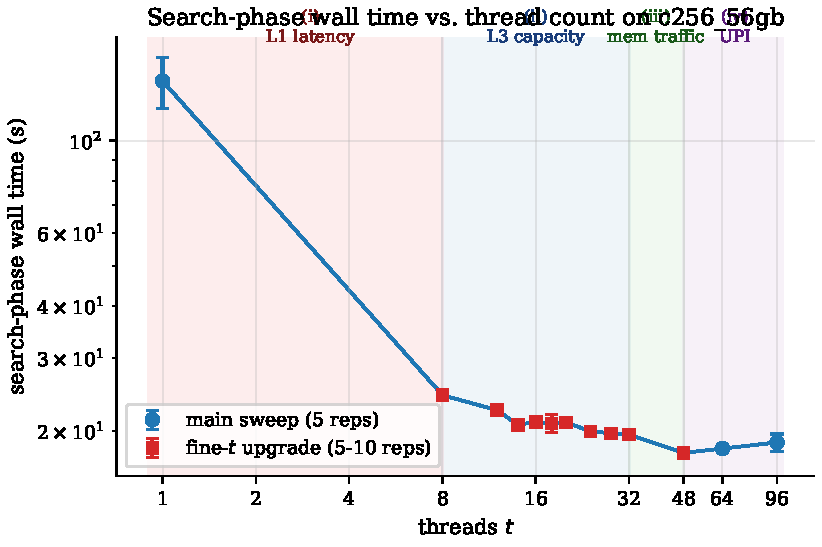
\includegraphics[width=0.9\linewidth]{img/gen/ch4_four_ceilings.pdf}
  \caption{Search-phase wall time of the default (SoA + f32) build on \texttt{c256\_56gb} across thread counts. Both axes are log-scaled. Shaded areas signify the regimes in which each ceiling binds: (i) single-thread compute / L1 latency at $t \leq 8$, (ii) shared L3 capacity at $t \in [8, 32]$, (iii) on-socket memory-traffic pressure at $t \in [32, 48]$, and (iv) cross-socket UPI interconnect at $t > 48$. Error bars show $95\%$ CIs from the 5-repetition measurements.}
  \label{fig:exp:four_ceilings}
\end{figure}

\section{Ceiling (i): Single-Thread Compute / L1 Latency\label{sec:exp:c1}}

Ceiling (i) is best tested in the single-thread regime, since there are no inter-thread effects to skew the measurement. We perform four ablation experiments addressing this ceiling from different angles: 
\begin{enumerate}
  \item AVX-512 leaf-stage SIMD (§\ref{sec:exp:c1:simd})
  \item 8-way pipelined batch-search (§\ref{sec:exp:c1:batch})
  \item 16-query horizontal-SIMD lockstep (§\ref{sec:exp:c1:horizontal})
  \item PGM learned-index (§\ref{sec:exp:c1:pgm})
\end{enumerate}

The results are null or marginal. A fifth latency-side variant, 4-way branchless k-ary search, was evaluated in an earlier campaign and dropped from the final build.

\paragraph{The Dependent-Load Chain in \texttt{partition\_point}.}

The hot loop per-cluster is the two binary searches in \texttt{partition\_point} (§\ref{sec:bg:partition_point}). The first search is over the bin-boundary array, the second is over the column slice of the cluster. The size of the bin-boundary array is fixed at ${\sim}142$; the size of the column slice is $n_\text{hists}$. The first fits into two L1d cache lines, the second fits into L2 but exceeds L1d on the larger datasets. Each iteration of each search is a dependent load that must wait for the previous iteration to complete. This dependent load chain \emph{is} the wall time per cluster on this workload.

\subsection{Ablation A: AVX-512 Leaf-Stage SIMD\label{sec:exp:c1:simd}}

The \texttt{simd} feature replaces the last ${\sim}16$ elements of \texttt{partition\_point} with one AVX-512 vector compare. This does not alter the dependent-load chain above the leaf, but it removes the last ${\sim}16$ dependent loads from the chain, shaving one iteration's latency from the inner loop.

\begin{table}[H]
  \centering
  \caption{\texttt{simd} vs default, suppress mode, median of 5. Ratio $<$ 1 means \texttt{simd} faster.}
  \label{tab:simd}
  \begin{tabular}{lrrrrrr}
    \toprule
    Dataset & $t{=}1$ & $t{=}8$ & $t{=}16$ & $t{=}32$ & $t{=}64$ & $t{=}96$ \\
    \midrule
    \texttt{c256\_10gb} & $1.04\times$ & $1.00\times$ & $0.98\times$ & $1.03\times$ & $0.97\times$ & $0.93\times$ \\
    \texttt{c256\_30gb} & $1.03\times$ & $1.01\times$ & $1.02\times$ & $1.00\times$ & $0.90\times$ & $0.95\times$ \\
    \texttt{c256\_56gb} & $1.07\times$ & $0.93\times$ & $1.04\times$ & $0.94\times$ & $0.96\times$ & $0.99\times$ \\
    \bottomrule
  \end{tabular}
\end{table}

The range of $0.90$--$1.07\times$ is within run-to-run noise across all 18 cells. \emph{SIMD} is not a ceiling-(i) win. The leaf vectoriser's job (removing the last ${\sim}16$ dependent loads) is correct, but it does not address the part of the dependency chain, that is the bottleneck. 

\subsection{Ablation B: 8-Way Batch-Search\label{sec:exp:c1:batch}}

\texttt{batch-search} is a columnar-only feature (mutually exclusive with \texttt{horizontal-\allowbreak simd}) that pipelines eight binary searches through the CPU's MSHR (Miss Status Holding Register) budget, sharing early-stage midpoint loads. Since queries are grouped by bin index $k^*$, it is only meaningful inside the column-centric engine. We compare to the columnar default.

\begin{table}[H]
  \centering
  \caption{\texttt{batch-search} vs \texttt{columnar-default}, suppress mode, median of 5. Ratio $<$ 1 means \texttt{batch-search} faster.}
  \label{tab:batchsearch}
  \begin{tabular}{lrrrrrr}
    \toprule
    Dataset & $t{=}1$ & $t{=}8$ & $t{=}16$ & $t{=}32$ & $t{=}64$ & $t{=}96$ \\
    \midrule
    \texttt{c256\_10gb} & $0.98\times$ & $1.05\times$ & $1.02\times$ & $1.00\times$ & $0.97\times$ & $1.01\times$ \\
    \texttt{c256\_30gb} & $1.09\times$ & $1.05\times$ & $1.05\times$ & $0.98\times$ & $1.00\times$ & $1.00\times$ \\
    \texttt{c256\_56gb} & $0.99\times$ & $1.01\times$ & $0.96\times$ & $0.99\times$ & $1.01\times$ & $0.99\times$ \\
    \bottomrule
  \end{tabular}
\end{table}

Across all 18 cells, the range is $0.96$--$1.09\times$, indistinguishable from noise, for the main workload \emph{c256\_56gb} the range is even tighter at $\pm 4\%$. 

This does not mean that \texttt{batch-search} is broken, the dependent-load chain above the leaf is not the bottleneck. The ceiling-(i) hypothesis is falsified.

\subsection{Ablation C: Horizontal-SIMD Lockstep\label{sec:exp:c1:horizontal}}

\texttt{horizontal-simd} \cite{polychroniou_2014} is columnar-only (mutually exclusive with \texttt{batch-search}). It vectorises 16 queries' bisection trees in tandem through one column, rather than within a single query. Structurally different from \texttt{simd}, but identical conclusion: the dependent-load chain above the leaf is not the bottleneck.

\begin{table}[H]
  \centering
  \caption{\texttt{horizontal-simd} vs \texttt{columnar-default}, suppress mode, median of 5. Ratio $<$ 1 means \texttt{horizontal-simd} faster.}
  \label{tab:horizsimd}
  \begin{tabular}{lrrrrrr}
    \toprule
    Dataset & $t{=}1$ & $t{=}8$ & $t{=}16$ & $t{=}32$ & $t{=}64$ & $t{=}96$ \\
    \midrule
    \texttt{c256\_10gb} & $0.95\times$ & $1.03\times$ & $1.06\times$ & $1.05\times$ & $0.96\times$ & $1.00\times$ \\
    \texttt{c256\_30gb} & $1.07\times$ & $1.06\times$ & $1.12\times$ & $1.03\times$ & $0.95\times$ & $1.00\times$ \\
    \texttt{c256\_56gb} & $1.02\times$ & $1.00\times$ & $0.99\times$ & $1.01\times$ & $0.98\times$ & $1.00\times$ \\
    \bottomrule
  \end{tabular}
\end{table}

Across all 18 cells, the range is $0.95$--$1.12\times$, which fits within the run-to-run noise. It does show a mild regression signature at intermediate $t$ on \texttt{c256\_30gb} where the L3-capacity ceiling begins to bind (§\ref{sec:exp:c2}). 

\subsection{Ablation D: PGM Learned Index\label{sec:exp:c1:pgm}}

\texttt{pgm} replaces binary-search with a learned-index segment lookup plus a small scan. The mechanism is described in §\ref{sec:method:impl:variants}. It was tested in all engines (row-centric, column-centric, query-batch) and the measurement here uses the row-centric default.

The dependent loads per cluster drop to $O(\log \log n)$ (Since the PGM segment lookup is near constant time) as intended, but wall does not move because wall was not bounded by those cycles to begin with. If ceiling~(i) bound, this would be the most direct attack possible.

\begin{table}[H]
  \centering
  \caption{\texttt{pgm} vs \texttt{default} (row-centric), suppress mode, median of 5. Ratio $<$ 1 means \texttt{pgm} faster.}
  \label{tab:pgm}
  \begin{tabular}{lrrrrrr}
    \toprule
    Dataset & $t{=}1$ & $t{=}8$ & $t{=}16$ & $t{=}32$ & $t{=}64$ & $t{=}96$ \\
    \midrule
    \texttt{c256\_10gb} & $1.12\times$ & $1.02\times$ & $1.00\times$ & $1.03\times$ & $1.05\times$ & $0.92\times$ \\
    \texttt{c256\_30gb} & $1.02\times$ & $1.13\times$ & $0.96\times$ & $1.05\times$ & $1.12\times$ & $0.92\times$ \\
    \texttt{c256\_56gb} & $0.91\times$ & $1.10\times$ & $1.00\times$ & $0.95\times$ & $0.99\times$ & $0.97\times$ \\
    \bottomrule
  \end{tabular}
\end{table}

Across all $18$ cells, the range is $0.91$--$1.13\times$. No single cell is an unambiguous win. Our largest win ($-9\%$ at \texttt{c256\_56gb} $t=1$) is matched by a similar-sized loss ($+13\%$ at \texttt{c256\_30gb} $t=8$). Perf counters confirm the $\log_2 n$ dependent-load cycles per cluster drop to $O(\log \log n)$ as intended, but since the dependent-load chain was not the bottleneck, wall does not move.

\subsection{Mechanism Evidence\label{sec:exp:c1:mechanism}}

Hot-loop counters Per-cluster on the default build (single thread) show the dependent-load chain dominates cycle budget. IPC is $1.80$ on \texttt{c256\_10gb}, $1.93$ on \texttt{c256\_30gb}, $1.87$ on \texttt{c256\_56gb}, all comfortably below the retirement ceiling and points to a load-latency-bound loop. The L1d miss-per-load rate at $t{=}1$ is $\sim\!0.49$--$0.68\%$ across the three datasets. Neither the misprediction rate nor the L1d-miss rate exceed the noise floor that the ablations were designed to reduce.

This resolves the apparent tension with the chain being the wall time: the binding quantity is the \emph{number} of dependent chains, one per cluster, not the depth or throughput of any single chain (which scales only as $\log_2$ of the bins per cluster). The four ablations shorten or pipeline individual chains; none of them reduces the count. That is why they all measure null.

Ceiling~(i) is part of the ceiling taxonomy due to it being the most commonly assumed default ceiling in the published literature on in-memory percentile and binary-search workloads. Kim et al.'s FAST index~\cite{kim_2010} explicitly co-optimises for cache-line, page, and SIMD width on the assumption that L1-latency and CMOV-chain length bind search cost, Khuong and Morin~\cite{khuong_morin_2017} benchmark array layouts under the same assumption, Ferragina and Vinciguerra's PGM~\cite{ferragina_2020} addresses the $\log_2 n$ dependent-load chain as its whole motivation, and Schlegel et al.'s SIMD $k$-ary search~\cite{schlegel_2009} treats the same chain as the cost to be shortened.

Our falsification of ceiling~(i) is what gives credit to the other ceilings and gives us the opportunity to set aside the single-thread compute assumption and reason about the other ceilings. This negative result is positive evidence about binding constraints.

\section{Ceiling (ii): Shared L3 Capacity\label{sec:exp:c2}}

The aggregate per-thread working set sums above the L3 shared capacity of $105$\,MiB per socket at moderate thread counts on the \emph{larger} datasets. We observe a thread-scaling curve that shows a bend before saturating the cores. Optimisations that shrink the per-thread footprint should improve this ceiling; optimisations that expand it should worsen it. The mechanism reading (§\ref{sec:exp:c2:mechanism}) refines this picture: what binds at moderate $t$ is regime-dependent, allocator-arena contention on dense clusters and aggregate L3 footprint at the sparser OOD density.

\subsection{SoA vs AoS\label{sec:exp:c2:soa}}

The default uses SoA. The \texttt{aos} feature is the negative control: every cache line loaded during the search now also carries an unused 32-bit ID field, halving the useful values per line.

\begin{table}[H]
  \centering
  \caption{\texttt{aos} vs default, suppress mode, median of 5 reps. Ratio $>$ 1 means \texttt{aos} slower; ratio $<$ 1 means \texttt{aos} \emph{faster} (bold cells).}
  \label{tab:aos}
  \begin{tabular}{lrrrrrr}
    \toprule
    Dataset & $t{=}1$ & $t{=}8$ & $t{=}16$ & $t{=}32$ & $t{=}64$ & $t{=}96$ \\
    \midrule
    \texttt{c256\_10gb} & $1.11\times$ & $1.05\times$ & $1.03\times$ & $\mathbf{0.98\times}$ & $1.07\times$ & $1.09\times$ \\
    \texttt{c256\_30gb} & $1.09\times$ & $1.07\times$ & $1.04\times$ & $1.06\times$ & $1.12\times$ & $\mathbf{0.94\times}$ \\
    \texttt{c256\_56gb} & $1.03\times$ & $1.17\times$ & $1.02\times$ & $1.00\times$ & $\mathbf{0.96\times}$ & $\mathbf{0.99\times}$ \\
    \bottomrule
  \end{tabular}
\end{table}

The primary workload \texttt{c256\_56gb} observes a $+17\%$ penalty at $t=8$ in the L3-capacity regime, but then flips to a small $-4\%$ gain at $t=64$. We do not consider this flip run-to-run noise, but an indicator of a ceiling-(ii)$\to$ceiling-(iii) transition of the binding constraint. AoS is negatively impacted  by the doubled per-line footprint in the L3-capacity regime, as confirmed by an $\sim\!+0.05$\, L1d-miss-per-instruction increase at $t=8$ versus SoA and the roughly doubled per-socket L3 working set at $t \in [8, 32]$.

AoS no longer becomes the binding cost, once on-socket memory-traffic pressure binds at $t \ge 48$, since the higher spatial locality of the interleaved (AoS) layout on the ID emit leaves a bit of room for improvement. We observe this also on \texttt{c256\_30gb} (t=96 flips to $-6\%$) but not on \texttt{c256\_10gb}, since its working set stays L2-resident, ceiling~(ii) never binds. SoA continues to be the right default for the composed bundle at $t=16$ where the wall budget matters most, but the layout choice is regime-conditional, rather than absolute.

Figure~\ref{fig:exp:aos_flip} shows the same measurement as a delta versus default across the finer thread sweep on \texttt{c256\_56gb}.

\begin{figure}[H]
  \centering
  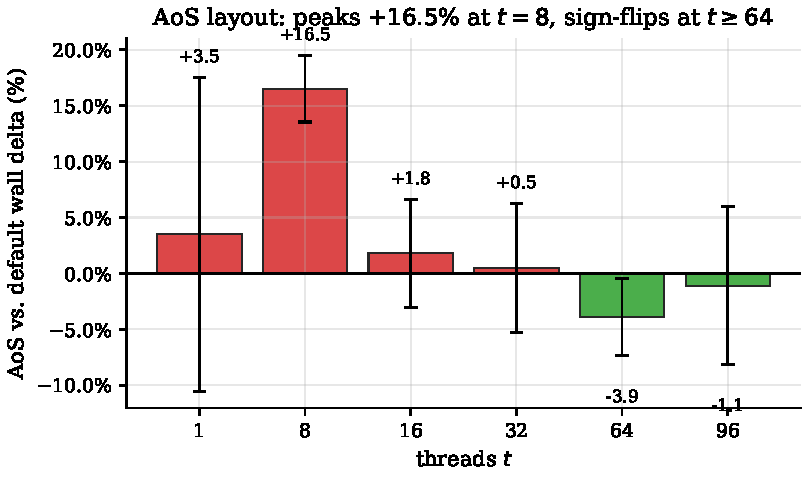
\includegraphics[width=0.9\linewidth]{img/gen/ch4_aos_flip.pdf}
  \caption{AoS layout wall-time delta versus default (SoA + f32) on \texttt{c256\_56gb} across threads. Red bars: AoS slower. Green bars: AoS faster. Error bars show $95\%$ CIs propagated through the delta computation.}
  \label{fig:exp:aos_flip}
\end{figure}

\subsection{f16 Footprint Halving\label{sec:exp:c2:f16}}

\texttt{f16} stores values as 16-bit half-precision floats that dequantise during comparison. We predict that \texttt{f16} wins in the regime where the f32 footprint exceeds L3 per socket but the f16 footprint fits, with the win largest at moderate $t$ on the larger datasets.

\begin{itemize}
  \item Standalone on \texttt{c256\_56gb}: no cell shows a statistically significant \texttt{f16} win. Figure~\ref{fig:exp:f16_finet} shows two significant losses at $t{=}8$ and $t{=}14$, every other cell in the $10$-rep fine-$t$ sweep straddles zero.
  \item Standalone on \texttt{c256\_30gb}: also no clear win. Deltas range from $-12\%$ (at $t{=}96$) to $+3.5\%$ (at $t{=}8$). The predicted L3-footprint win at $t{=}16$ ($+3.1\%$) is a small loss instead.
  \item Inside the bundled \bcombo{} build at $t{=}16$ on \texttt{c256\_56gb}, the bundle runs at $0.773\times$ default wall ($22.7\%$ speedup).
  \item \texttt{f16} isolation measures \texttt{f16}'s contribution to the bundle: we find a \emph{regime-dependent sign reversal} on the primary workload; \texttt{c256\_56gb} at $t{=}16$, \bcombo{} without \texttt{f16} at $13.54$\,s is $15.6\%$ \emph{faster} than \bcombo{} at $16.03$\,s meaning that \emph{f16} drags the net bundle down (and $-16.2\%$ at $t{=}32$, only at $t{=}64$ and $t{=}96$ does removing \texttt{f16} produce a small $\sim\!3\%$ cost). On the sparser OOD workload \texttt{c1024\_56gb} (§\ref{sec:exp:ood}) at the same $t{=}16$, removing \texttt{f16} costs $+20.9\%$, so \texttt{f16} saves $20.9\%$ inside the bundle.
  \item The reversal is \emph{density-dependent}. On \texttt{c256\_56gb} the per-cluster f32 slice ($\sim\!105$\,KiB) exceeds L1d and is L2-resident; halving it does not unlock a new cache-resident regime, while paying f16$\to$f32 conversion costs on every comparison. The mechanism is developed further in §\ref{sec:exp:c2:mechanism}.
  \item \texttt{f16} is a bundle drag that the other five features have to absorb. At the sparser OOD density, \texttt{f16} carries roughly a fifth of the bundle win.
\end{itemize}

\begin{figure}[H]
  \centering
  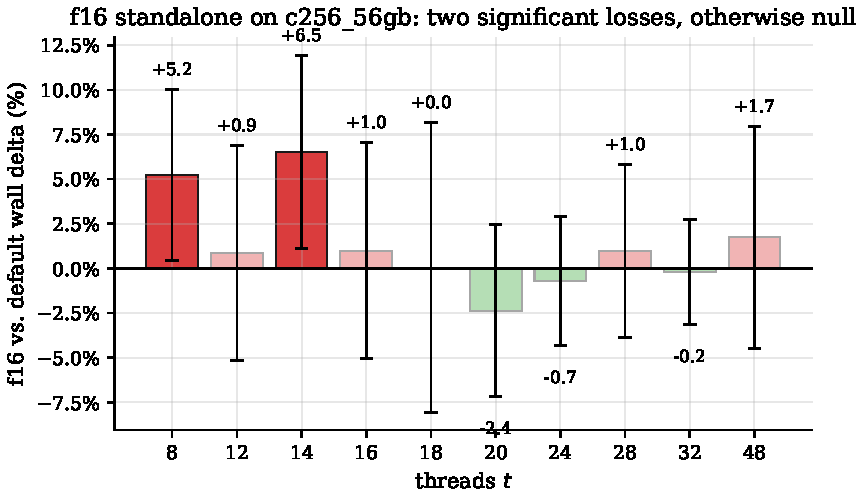
\includegraphics[width=0.9\linewidth]{img/gen/ch4_f16_finet.pdf}
  \caption{\texttt{f16} vs.\ default wall-time delta on \texttt{c256\_56gb}. Saturated bars mark cells where $t$ $95\%$ CI (dof $= n_a + n_b - 2$, §\ref{sec:method:ci}) excludes zero, pale bars are noise-band.}
  \label{fig:exp:f16_finet}
\end{figure}

 

\subsection{Pooled Output Buffer\label{sec:exp:c2:pooled}}

\texttt{pooled} is a bundle feature that pre-allocates the output buffer for each query, rather than allocating one per matching cluster. The intended mechanism is a smaller per-thread allocator footprint and elimination of the glibc arena mutex contention from §\ref{sec:exp:c2:mechanism}.

\begin{table}[H]
  \centering
  \caption{\texttt{pooled} vs default, suppress mode. Ratio $<1$ means \texttt{pooled} faster.}
  \label{tab:pooled}
  \begin{tabular}{lrrrrrr}
    \toprule
    Dataset & $t{=}1$ & $t{=}8$ & $t{=}16$ & $t{=}32$ & $t{=}64$ & $t{=}96$ \\
    \midrule
    \texttt{c256\_10gb} & $\mathbf{0.51\times}$ & $\mathbf{0.75\times}$ & $\mathbf{0.94\times}$ & $0.99\times$ & $1.03\times$ & $\mathbf{0.88\times}$ \\
    \texttt{c256\_30gb} & $\mathbf{0.57\times}$ & $\mathbf{0.73\times}$ & $1.00\times$ & $0.98\times$ & $1.07\times$ & $1.42\times$ \\
    \texttt{c256\_56gb} & $\mathbf{0.53\times}$ & $\mathbf{0.66\times}$ & $\mathbf{0.80\times}$ & $\mathbf{0.95\times}$ & $\mathbf{0.93\times}$ & $1.02\times$ \\
    \bottomrule
  \end{tabular}
\end{table}

Measurements confirm the arena-mutex mechanism at scale. On \texttt{c256\_56gb} \texttt{pooled} standalone wins $-46.9\%$ at $t{=}1$, $-34.1\%$ at $t{=}8$, and $-20.2\%$ at $t{=}16$. On the primary workload at $t{=}16$, \texttt{pooled} carries essentially the entire bundle win, with the other five features (including \texttt{f16}) providing a small net loss that \texttt{pooled}'s cushion absorbs.

The wins compress at higher $t$ on the two smaller datasets and even flip negative on \texttt{c256\_30gb} at $t{=}96$. At low $t$ the allocator arena mutex serialises threads on the shared glibc arena, at high $t$ other ceilings (memory-traffic pressure, UPI) dominate and the arena is no longer the binding cost, so \texttt{pooled}'s cushion has less to protect against.

\paragraph{Bundle-minus-pooled isolation}

The direct \bcombo{}-minus-\texttt{pooled} sweep on \texttt{c256\_56gb} reveals a shape as regime-dependent as the \texttt{f16} isolation of §\ref{sec:exp:c2:f16}:

\begin{table}[H]
  \centering
  \caption{\bcombo{}-minus-\texttt{pooled} vs full \bcombo{}. Positive removal cost means \texttt{pooled} was helping the bundle, negative means \texttt{pooled} was \emph{hurting} it.}
  \label{tab:pooled_isolation}
  \footnotesize
  \begin{tabular}{lrrrrrr}
    \toprule
    & $t{=}1$ & $t{=}8$ & $t{=}16$ & $t{=}32$ & $t{=}64$ & $t{=}96$ \\
    \midrule
    \bcombo{} wall (s)          & $117.6$ & $18.9$ & $16.0$ & $16.6$ & $19.1$ & $20.5$ \\
    \texttt{bs}-minus-\texttt{pooled} wall (s) & $181.9$ & $26.0$ & $16.7$ & $15.1$ & $18.5$ & $20.9$ \\
    \texttt{pooled} bundle contribution & $+54.7\%$ & $+37.1\%$ & $+4.4\%$ & $\mathbf{-9.4\%}$ & $\mathbf{-3.2\%}$ & $+1.8\%$ \\
    \bottomrule
  \end{tabular}
\end{table}

This is a second inside-bundle sign-flip alongside \texttt{f16}'s (§\ref{sec:exp:c2:f16}): an optimisation that decisively wins standalone can turn into a bundle drag at a different regime cell. The direction of the drag is set by which ceiling binds at the composition. §\ref{sec:exp:c2:mechanism} dives deeper into the two-feature reversal mechanism.

\subsection{Mechanism Reading\label{sec:exp:c2:mechanism}}

Ceiling~(ii) binds at moderate $t$ on the larger datasets. Although, this binding is less straightforward than pure L3 capacity. It is regime-dependent like the direct standalone and bundle-isolation measurements now let us name.

The first binding constraint on the  primary workload at moderate $t$ is allocator-arena mutex contention instead of L3 capacity. \texttt{pooled}'s job was to address the mutex by removing per-cluster vector allocation, which it wins $-20.2\%$ at $t{=}16$. After that, the two direct bundle isolations show that neither \texttt{f16} nor \texttt{pooled} compose cleanly.

\begin{itemize}
  \item \texttt{f16} standalone wins nothing at any $t$ on \texttt{c256\_56gb}, and inside the bundle it is a $+15.6\%$ drag at $t{=}16$: removing \texttt{f16} makes the bundle faster.
  \item \texttt{pooled} standalone wins $-20.2\%$ at $t{=}16$, but inside the bundle its contribution collapses to $+4.4\%$ at $t{=}16$ and \emph{flips sign} at $t{=}32$--$64$, where removing \texttt{pooled} makes the bundle $-9.4\%$/$-3.2\%$ faster.
\end{itemize}

As formalised in §\ref{sec:exp:negcomp}, the ceiling that binds at a given regime cell is not necessarily the same ceiling that bound at a different regime cell. The ceiling that binds at $t{=}16$ is allocator-arena mutex contention, which \texttt{pooled} addresses. The ceiling that binds at $t{=}32$--$64$ is on-socket memory-traffic pressure, which \texttt{pooled} does not address and whose contention costs it adds to.

For the OOD workload \texttt{c1024\_56gb}, we observe a different ceiling-(ii) mechanism. A per-cluster f32 slice ($\sim\!33$\,KiB) fits in L1d, but the $610$ effective clusters (vs.\ $191$ on \texttt{c256\_56gb}) mean the aggregate cluster-loop working set is proportionally larger. \texttt{f16}'s halving pays back by $\sim\!20\%$ inside the bundle. Ceiling (ii) thus covers arena-mutex serialisation on dense clusters, L3-aggregate footprint pressure on sparse many-clusters, showing that the ceiling is not a single mechanism but a regime-dependent set of mechanisms. We can separate the two with our standalone-vs-bundle sign-flip on \texttt{f16} between the two workloads, which is the empirical evidence that they are separate.

Two mechanistic details to note:

\begin{itemize}
  \item \texttt{mimalloc} standalone \emph{hurts} at low-$t$ on \texttt{c256\_56gb} (+22\% at $t{=}1$ and $t{=}8$) but wins $-10\%$ at $t{=}32$. The regression at lower thread counts is likely due to mimalloc's per-thread arena warmup dominating.
  \item \texttt{pin-cores} standalone wins $-19\%$ at $t{=}32$ and is neutral to mildly negative at $t{=}64$--$96$. $t \geq 64$ is already contended by SMT threads on the same physical core, so \texttt{pin-cores} cannot help. 
\end{itemize}

We don't consider either \texttt{mimalloc} or \texttt{pin-cores} to be a ceiling-(ii) win in isolation, but they are both useful inside the bundle at their own regime cells.

\section{Ceiling (iii): On-Socket Memory-Traffic Pressure\label{sec:exp:c3}}

At high $t$ on the larger datasets, the DDR5 per-socket bandwidth budget (${\sim}300$\,GB/s) saturates. We observe \emph{anti-scaling}: wall-clock rises while cores are added past the saturation point. Optimisations that could improve this ceiling include reducing bytes-per-emit or bytes-per-comparison.

\paragraph{Anti-Scaling Signature.}\label{sec:exp:c3:anti}

Adding more cores does not add more bandwidth past the channel limit, and the cross-thread contention costs grow.

At \texttt{c256\_30gb} $t{=}96$, the default build takes $5.89$\,s, which is $+42\%$ slower than $t{=}64$ at $4.14$\,s.

Perf counters at $t=96$ on default \texttt{c256\_30gb}: IPC drops to $0.55$ from $1.93$ at $t=1$, and the LLC-miss count rises by $1.6\times$ between $t=64$ and $t=96$. The same dataset under \texttt{packed-ids} only goes $3.88$\,s $\rightarrow$ $4.70$\,s, a $+21\%$ slowdown over the same $t$ step.

\subsection{\texttt{packed-ids}: Bit-Packed Emit Phase\label{sec:exp:c3:packed}}

The \texttt{packed-ids} feature compresses the emit-phase ID bandwidth from $32$ bits per ID to ${\sim}20$ bits (the actual maximum global ID in the cluster). The decoder is $\sim\!3$ instructions per ID, the bandwidth saving is ${\sim}37\%$ on \texttt{c256\_10gb}.

\begin{table}[H]
  \centering
  \caption{\texttt{packed-ids} vs default, suppress mode, median of 5. Ratio $<$ 1 means \texttt{packed-ids} faster.}
  \label{tab:packed}
  \begin{tabular}{lrrrrrr}
    \toprule
    Dataset & $t{=}1$ & $t{=}8$ & $t{=}16$ & $t{=}32$ & $t{=}64$ & $t{=}96$ \\
    \midrule
    \texttt{c256\_10gb} & $0.94\times$ & $0.91\times$ & $1.00\times$ & $0.94\times$ & $1.04\times$ & $0.92\times$ \\
    \texttt{c256\_30gb} & $0.92\times$ & $0.86\times$ & $0.91\times$ & $0.95\times$ & $0.94\times$ & $\mathbf{0.80\times}$ \\
    \texttt{c256\_56gb} & $\mathbf{0.83\times}$ & $0.97\times$ & $0.96\times$ & $0.98\times$ & $0.91\times$ & $0.97\times$ \\
    \bottomrule
  \end{tabular}
\end{table}

Range $0.80$--$1.04\times$. Three cells show the largest wins with different mechanisms:

\begin{itemize}
  \item \textbf{30gb $t{=}96$ ($-20\%$).} bandwidth-saturation case. Default scales anti-monotonically ($t{=}64 \rightarrow t{=}96$: $4.15$\,s $\rightarrow$ $5.89$\,s), \texttt{packed-ids} is effective here since it reduces per-id bandwidth.
  \item \textbf{56gb $t{=}1$ ($-17\%$).} L3-capacity pressure at low $t$. The 56\,GB index footprint exceeds the $105$\,MiB shared LLC per socket even with one thread holding it. Reading $20$ bits/id instead of $32$ reduces capacity-miss rate, so each id costs fewer DRAM round-trips.
  \item \textbf{56gb $t{=}64$ ($-9\%$).} Bandwidth before HT-contention dominates, the saving partially translates into a wall win.
\end{itemize}

Once again, the win pattern follows regimes instead of mechanisms, which is why a ceiling-organised framing is useful.

\paragraph{\texttt{mimalloc}: Allocator Sub-Ceiling.}\label{sec:exp:c3:mimalloc}

\texttt{mimalloc} is a drop-in replacement for glibc malloc. It uses per-thread sharded free lists to reduce allocator contention. Calls are done across threads without a global mutex, which is the mechanism that matters at high $t$ on big data. \texttt{mimalloc} loses at low $t$ on \texttt{c256\_56gb}, wins at $t{=}32$, and drifts back to small losses at $t \geq 64$ . The $t{=}32$ win is the intended mechanism. It composes into the bundle in §\ref{sec:exp:c2:mechanism}.

\section{Ceiling (iv): Cross-Socket UPI Interconnect\label{sec:exp:c4}}

§\ref{sec:exp:c3} treats memory-traffic pressure as a single ceiling. The 8468H platform has two memory pipes: per-socket DDR5 (${\sim}300$\,GB/s) and the cross-socket Ultra-Path Interconnect. The NUMA placement probe in §\ref{sec:method:impl:numa} separates the two.

\subsection{Four-Config NUMA Probe and Results}

Four \texttt{numactl} configurations on \texttt{c256\_56gb} with \texttt{--features packed-ids}:

\begin{itemize}
  \item \textbf{A (unpinned).} Linux first-touch; default scheduler.
  \item \textbf{B (single-socket-clean).} \texttt{numactl --cpunodebind=0 --membind=0}. Memory and CPUs on node 0. Only feasible at $t \le 48$ (one socket of physical cores).
  \item \textbf{C (interleave).} \texttt{numactl --interleave=0,1}. Pages striped round-robin across nodes at 4\,KB granularity.
  \item \textbf{D (cross-socket forced).} \texttt{numactl --membind=0 --physcpubind=48..N}. Memory on node 0, CPUs on node 1. Worst case for UPI cost.
\end{itemize}

\begin{table}[H]
  \centering
  \caption{NUMA placement probe, \texttt{c256\_56gb}, \texttt{packed-ids} build, suppress mode, median of 5. Wall in seconds.}
  \label{tab:numa}
  \begin{tabular}{lrrrr}
    \toprule
    Config & $t{=}32$ & $t{=}48$ & $t{=}64$ & $t{=}96$ \\
    \midrule
    A (unpinned) & $19.28$ & $16.97$ & $18.19$ & $17.58$ \\
    B (single-socket node 0) & $\mathbf{16.77}$ & $\mathbf{15.04}$ & -- & -- \\
    C (interleave 0,1) & $25.87$ & $23.73$ & $22.91$ & $24.83$ \\
    D (cross-socket forced) & $19.08$ & $16.86$ & -- & -- \\
    \bottomrule
  \end{tabular}
\end{table}

We observe the following readings:

\begin{itemize}
  \item \textbf{(B vs A).} Single-socket beats unpinned by $11$--$13\%$ at matched thread count.
  \item \textbf{(D vs A).} Cross-socket-forced $\approx$ unpinned, within $1\%$.
  \item \textbf{(C vs A).} Interleave regresses by $26$--$41\%$. The naïve ``balance memory across sockets'' fix moves wall the wrong way at every thread count.
\end{itemize}

\textbf{(D vs A)} unpinned baseline already pays cross-socket UPI cost. At construction time, most of the index is on node 0, but at $t > 24$ many Rayon workers schedule onto node 1.


\textbf{(C vs A)} 4\,KB-granularity interleave fragments each working set, meaning that half the bytes are local, half remote. This is unpredictable per page, which defeats the hardware prefetcher's spatial stride and forces every cluster access to pay a $50\%$ cross-socket expectation. 

\section{Multi-Core Scaling and SMT Contention\label{sec:exp:scaling}}

The thread-scaling curve under the default build connects the four ceilings: it shows where each binds along the $t$ axis.

\begin{table}[H]
  \centering
  \caption{Default Rust build, suppress mode, median of 5. ``Best/$t{=}1$'' is the speedup at the best thread count vs $t{=}1$.}
  \label{tab:thread_scaling}
  \begin{tabular}{lrrrrrrrr}
    \toprule
    Dataset & $t{=}1$ & $t{=}8$ & $t{=}16$ & $t{=}32$ & $t{=}64$ & $t{=}96$ & best & best/$t{=}1$ \\
    \midrule
    \texttt{c256\_10gb} & $8.38$ & $1.88$ & $\mathbf{1.44}$ & $1.60$ & $1.92$ & $2.96$ & $t{=}16$ & $5.82\times$ \\
    \texttt{c256\_30gb} & $26.43$ & $5.36$ & $4.04$ & $\mathbf{3.93}$ & $4.14$ & $5.89$ & $t{=}32$ & $6.73\times$ \\
    \texttt{c256\_56gb} & $139.35$ & $24.78$ & $20.74$ & $19.36$ & $\mathbf{18.16}$ & $18.78$ & $t{=}64$ & $7.67\times$ \\
    \bottomrule
  \end{tabular}
\end{table}

Smaller datasets bend at lower thread counts because per-query work is shorter, more queries are in flight at any moment, and the working set exceeds the shared L3 sooner. 

On \texttt{c256\_10gb} we measure ${\sim}150\,\mu$s per query at $t=1$. At $t=96$ the per-thread work slices are so short that scheduling overhead and cross-thread contention dominate them; the working set itself stays cache-resident, so the bend is not a capacity effect (consistent with ceiling~(ii) never binding on this dataset, §\ref{sec:exp:c2:soa}).

On \texttt{c256\_56gb} we measure ${\sim}25$\,ms per query at $t=1$. Even at $t=96$ the in-flight footprint stays within L3 capacity, so the regression past $t=64$ is not ceiling (ii) but a mix of ceilings (iii) and (iv).

\subsection{HT-Sibling Contention and \texttt{pin-cores}\label{sec:exp:scaling:pin}}

Above $t=96$ the engine maps two Rayon workers onto SMT siblings of the same physical core, and they contend for L1d/L2. This is not prevented by the default Linux scheduler. The \texttt{pin-cores} feature uses \texttt{core\_affinity} to bind one worker per physical core.

Standalone on \texttt{c256\_56gb}, \texttt{pin-cores} wins at $t \leq 32$ and peaks at $-19.2\%$ at $t=32$. At $t=64$ it is neutral ($+1.2\%$); at $t=96$ it regresses to $+7\%$ ($20.10$\,s vs default $18.78$\,s).

Once all $96$ physical cores are pinned, the affinity mask cannot help further, and the pinning itself removes the scheduler's freedom to migrate threads off a bandwidth-contended socket.

Inside \bcombo{} the feature contributes usefully at moderate $t$ (§\ref{sec:exp:c2:pooled}).


\subsection{Nested Cluster Parallelism\label{sec:exp:scaling:clusterpar}}

Inside the per-query Rayon task, \texttt{cluster-par} adds a second Rayon scope that parallelises over clusters. The hypothesis is that nested work-stealing balances heterogeneous cluster cost better than flat per-query parallelism. The measurement falsifies this at $t \ge 16$:

\begin{table}[H]
  \centering
  \caption{\texttt{cluster-par} vs default. Ratio $>$ 1 means \texttt{cluster-par} slower.}
  \label{tab:clusterpar}
  \begin{tabular}{lrrrrrr}
    \toprule
    Dataset & $t{=}1$ & $t{=}8$ & $t{=}16$ & $t{=}32$ & $t{=}64$ & $t{=}96$ \\
    \midrule
    \texttt{c256\_10gb} & $0.84\times$ & $0.97\times$ & $1.17\times$ & $1.30\times$ & $\mathbf{1.77\times}$ & $\mathbf{1.82\times}$ \\
    \texttt{c256\_30gb} & $0.74\times$ & $0.95\times$ & $1.19\times$ & $1.87\times$ & $\mathbf{3.70\times}$ & $\mathbf{2.67\times}$ \\
    \texttt{c256\_56gb} & $0.89\times$ & $1.13\times$ & $1.37\times$ & $1.15\times$ & $\mathbf{2.67\times}$ & $\mathbf{2.96\times}$ \\
    \bottomrule
  \end{tabular}
\end{table}

Up to $3.7\times$ slower than default.

 At $t \ge 8$ the outer per-query parallelism already saturates the pool. This does not allow the outer query to be parallelised. Every thread is already busy. The inner Rayon scope adds overhead for task-creation ($\sim\,\mu$s per task $\times$ $\sim\!150$ clusters $\times$ $10\,000$ queries $= 1.5$M extra tasks), lock contention, cache-line ping-pong, and memory bandwidth contention. Nested parallelism on top of saturated parallelism is just overhead.

\section{The Work-Fragmentation Regime\label{sec:exp:wf}}

A new bottleneck appears at high $t$ after optimisations that compress per-cluster work. The cluster cold-load itself becomes the dominant cost. Each rayon task has to process a query across all clusters in a sequential order, that means transitioning from one cluster to the next pays a cold-load worth of L2-to-L3 traffic for the next cluster's data. With small per-cluster work (after f16, packed-ids, etc.), that transition cost grows as a fraction of the total wall time. The work-fragmentation regime is defined as the regime where the cluster cold-load dominates the per-query work.

\subsection{Column-Centric Engine\label{sec:exp:wf:columnar}}

The column-centric engine (§\ref{sec:method:impl:columnar}) inverts the loop structure. Clusters become the outer parallel iterator and all queries for a cluster are processed inside, grouped by their bin index $k^*$.

\begin{itemize}
  \item At $t=1$ on \texttt{c256\_56gb}, we observe a $2.22\times$ speedup ($-54.9\%$ wall) for columnar vs default row-centric, marking it as the only regime where columnar is faster than row-centric.
  \item At $t \geq 8$ on \texttt{c256\_56gb}, the sign flips and the loss is large, losing by $+83\%$ at $t=8$, and by $t=16$--$96$ the loss gets to $+109\%$ to $+125\%$. The mechanism behind this is that the Rayon task count is bounded by the number of clusters, which is ${\sim}191$ on \texttt{c256\_56gb}. At a thread count of $t \geq 8$, the work distribution becomes coarse-grained relative to the thread pool. A few clusters make the tail of the work distribution, and the load imbalance across clusters dominates the per-cluster cache-reuse within one cluster.
  \item The same sign flip is observed on the smaller datasets, but at lower $t$ because the per-cluster work is smaller and the cross-cluster load imbalance dominates earlier.
\end{itemize}

We conclude that the columnar engine is only faster than row-centric in the single-thread corner of the dispatch grid (§\ref{sec:exp:dispatch}), where its per-cluster amortisation cannot be beaten. 

\subsection{Query-Batch: Cold-Load Amortisation\label{sec:exp:wf:qb}}

\texttt{query-batch} (§\ref{sec:method:impl:qbatch}) aims to keep the fine-grained parallelism that row-centricism provides, but amortises the cluster cold-load across multiple queries. This is done by grouping $K$ queries into a batch, and processing them together in the cluster loop. Making the outer iterator \texttt{par\_chunks(K)} and the inner loop clusters-outer/queries-inner.

\begin{table}[H]
  \centering
  \caption{$K$-sensitivity at $t{=}96$ on \texttt{c256\_56gb}, suppress mode, median of 5.}
  \label{tab:qb_k}
  \begin{tabular}{rrrr}
    \toprule
    $K$ & wall & vs default ($18.78$\,s) & vs \bcombo{} ($20.52$\,s) \\
    \midrule
    $16$ & $19.92$ & $+6.1\%$ & $-2.9\%$ \\
    $32$ & $20.28$ & $+8.0\%$ & $-1.2\%$ \\
    $64$ & $20.47$ & $+9.0\%$ & $-0.3\%$ \\
    $128$ & $\mathbf{16.17}$ & $\mathbf{-13.9\%}$ & $\mathbf{-21.2\%}$ \\
    $256$ & $16.44$ & $-12.5\%$ & $-19.9\%$ \\
    \bottomrule
  \end{tabular}
\end{table}

When this regime produces fewer batches than threads, it leaves workers idle. The sweet spot is where the amortisation benefit of $K$ queries outweighs the cost of leaving some threads idle.
Optimal $K$ grows with $t$ and the per-query work. 

query-batch turns one cluster cold-load into $K$ warm uses. Query-batch breaks the anti-scale at high $t$ on \texttt{c256\_56gb}. It is the only ablation in the campaign that does so.

\subsection{Morsel Scheduling\label{sec:exp:wf:morsel}}

Morsel-driven scheduling (§\ref{sec:method:impl:morsel}) is a finer-grained mechanism than query-batch. It aims to keep all workers busy by letting them steal morsels of work from each other, instead of leaving them idle when the number of batches is less than the number of threads. a morsel scheduler would force all workers to (mostly) drain cluster $c$ before advancing, keeping the data shared in L3 across all workers for the duration of phase $c$.

\begin{table}[H]
  \centering
  \caption{\texttt{c256\_56gb}, suppress mode, median of 5. Wall in seconds. Best per row in bold.}
  \label{tab:morsel}
  \footnotesize
  \begin{tabular}{rrrrrrr}
    \toprule
    $t$ & default & \bcombo{} & packed-ids & qbatch $K{=}128$ & morsel & morsel vs best \\
    \midrule
    $32$ & $19.36$ & $\mathbf{16.63}$ & $18.93$ & $17.22$ & $18.57$ & $+11.7\%$ \\
    $64$ & $18.15$ & $19.10$ & $\mathbf{16.59}$ & $16.89$ & $18.09$ & $+9.0\%$ \\
    $96$ & $18.78$ & $20.52$ & $18.23$ & $\mathbf{16.17}$ & $18.05$ & $+11.6\%$ \\
    \bottomrule
  \end{tabular}
\end{table}

Morsel beats default at every cell (up to $\sim\!4\%$ faster) but fails to acquire the same wins against the regime-best. This suggests that the engine is neither bandwidth-bound nor work-fragmentation-bound at this scale. This signature signals that morsel's coordination cost matches the saving it was designed to deliver. We already absorb cross-task cold-loads at the L3 layer without explicit coordination, so the morsel scheduler finds no residual to amortise.

\section{Negative Composability: A Structural Pattern\label{sec:exp:negcomp}}

The instances of negative composability share the same shape: a coarse mechanism captures the dominant share of what a finer mechanism is designed to recover, and the finer mechanism does not compose. This happens due to the finer mechanism's overhead, which finds no residual headroom to recover and emerges as net cost.

\subsection{Five Instances on Five Axes\label{sec:exp:negcomp:instances}}

\begin{table}[H]
  \centering
  \caption{The five negative-composability instances. Read each row as: baseline composition plus the finer ablation layered on top of it. The full mechanism stories are developed in §\ref{sec:exp:negcomp:arithmetic} and the section cited per row.}
  \label{tab:negcomp}
  \footnotesize
  \begin{tabular}{>{\raggedright\arraybackslash}p{0.20\linewidth}>{\raggedright\arraybackslash}p{0.26\linewidth}>{\raggedright\arraybackslash}p{0.15\linewidth}>{\raggedright\arraybackslash}p{0.28\linewidth}}
    \toprule
    Composition & Binding ceiling at baseline & Intended axis & Outcome \\
    \midrule
    \bcombo{} $+$ \texttt{packed-ids} (§\ref{sec:exp:c3:packed}) & mem-traffic; \texttt{f16} and \texttt{pooled} had already collected it & emit-phase ID bandwidth & NEG in 12/18 cells, up to $+24\%$ at low $t$ \\
    \bcombo{} $+$ qbatch $K{=}128$ (§\ref{sec:exp:wf:qb}) & mem-traffic; \texttt{f16} halved the cold-load size & cold-load occurrences & NEG at every \texttt{c256\_56gb} cell, $+8$ to $+32\%$ \\
    qbatch $+$ morsel (§\ref{sec:exp:wf:morsel}) & shared L3 absorbs cross-task cold-loads & cross-worker coordination & NEG at every cell, $+8$ to $+12\%$ \\
    \texttt{packed-ids} $+$ \texttt{local-ids} (§\ref{sec:exp:reindex}) & mem-traffic; the $\text{bw}{\approx}20$ decoder had collected the read-side saving & read-side bandwidth & NEG, $+186$ to $+245\%$ at $t \in [8,64]$; dTLB miss rate $52\times$ (§\ref{sec:exp:reindex:mechanism}) \\
    first-touch $+$ interleave (§\ref{sec:exp:c4}) & UPI; first-touch keeps each cluster node-contiguous & memory-locality balancing & NEG at every cell, $+26$ to $+41\%$; defeats the prefetcher \\
    \bottomrule
  \end{tabular}
\end{table}

Five axes: emit-phase bandwidth, cluster cold-load size, cross-worker coordination, decoder access pattern, memory-locality fragmentation, all grounding negative results. This recurring pattern is a structural property of the workload and the hardware instead of an ablation quirk.

\subsection{Arithmetic Pitfalls\label{sec:exp:negcomp:arithmetic}}

Each of the five ablations is justified by reasoning that ignores the multi-thread interaction with the baseline.

\texttt{packed-ids} saves on emit-id bandwidth, a measurable fraction of total per-emit memory traffic. Prediction of a positive composition with \bcombo{}, but \texttt{pooled} had already defused the emit-allocator pressure that was the binding constraint.

\texttt{query-batch} amortises cluster cold-load across $K$ queries. Prediction of a positive composition with \texttt{f16}, but \texttt{f16} already halved the per-cluster cold-load size,so route-preprocessing plus per-batch state cost exceeds it. 

\texttt{Morsel-style}  phase coordination amortises cluster cold-load \emph{across} workers on top of qbatch's in-task amortisation. Prediction of a positive composition, but the shared $105$\,MiB L3 absorbs cross-task cold-loads without explicit coordination. There was also a prediction of a positive composition with \texttt{packed-ids}, but the $\text{bw}{=}13$ decoder access-pattern drives dTLB-miss rate up $\sim\!52\times$ per instruction (§\ref{sec:exp:reindex:mechanism}), drowning the bandwidth saving in TLB-walk stalls. 

Memory interleave distributes pages round-robin across nodes.Prediction of a positive composition against unpinned first-touch, but first-touch already keeps each cluster's bytes contiguous on one node, and 4\,KB-granularity interleave defeats the prefetcher.

The first ablation moved the binding constraint to a different axis, and the second ablation pays its own cost without recovering against any residual on the \emph{new} binding axis.

\subsection{Pre-Flight Ceiling Identification\label{sec:exp:negcomp:preflight}}

The traditional ablation methodology assumes that the ablation's intended addressed axis is independently informative. We falsify that assumption on hardware-near workloads, as an ablation composes depends on the binding ceiling at the target composition, not the default build.

The pre-flight check of the five instances is a five-step process:

\begin{enumerate}
  \item Identify the binding ceiling at the \emph{target} composition baseline via a perf-counter probes.
  \item Verify that the ablation's axis still binds at that composition.
  \item If the axis does still bind, predict the saving via bandwidth-budget arithmetic.
  \item Measure across the regime cells where the ceiling binds. Use a decomposition to separate the ablation's intended saving from its bookkeeping cost.
  \item If the composition is negative, the story counts as a result, not just the delta wall time.
\end{enumerate}


\subsection{Methodology and Recipe\label{sec:exp:negcomp:methodology}}

The description of a deployment recipe in §\ref{sec:exp:dispatch} serves as a useful artefact for this codebase; while the methodology in §\ref{sec:exp:negcomp} is a useful artefact for future ablation campaigns on hardware-near workloads.

Our finding is ``the pattern exists on hardware-near composition'', instead of the black-and-white ``every ablation composes negatively''. A falsification to this pattern would be an ablation that composes positively against a baseline whose binding ceiling it explicitly does not address.

\section{Per-Cluster Reindexing (Falsified Prediction)\label{sec:exp:reindex}}

§\ref{sec:exp:c3:packed}'s \texttt{packed-ids} addressed the emit-phase bandwidth by bit-packing global histogram IDs at ${\sim}20$ bits. An obvious continuation would have been per-cluster local IDs; since each cluster holds at most a few thousand histograms, a local-id encoding could drop us to ${\sim}13$ bits, saving an additional $35\%$ on the read side. This prediction was falsified by the controlled measurement in this section. 

We consider this the most detailed example of the multi-variant decomposition that the pre-flight methodology (§\ref{sec:exp:negcomp:preflight}) recommends.

\subsection{Pre-Registered Prediction}

Per-emit memory traffic in row-centric SoA, written as (read width $+$ write width) over the per-emit operation:

\begin{table}[H]
  \centering
  \caption{Pre-registered bandwidth-budget arithmetic for the four variants.}
  \label{tab:reindex_budget}
  \footnotesize
  \begin{tabular}{lrrrr}
    \toprule
    Variant & read (bits) & write (bits) & total & vs default \\
    \midrule
    default (32-bit unpacked) & $32$ & $32$ & $64$ & baseline \\
    \texttt{packed-ids} (20-bit global) & $20$ & $32$ & $52$ & $-19\%$ \\
    \texttt{local-ids} (13-bit + lookup $\rightarrow$ 32-bit global) & $13$ & $32$ & $\mathbf{45}$ & $\mathbf{-30\%}$ \\
    \texttt{local-ids-bench} (13-bit, no lookup) & $13$ & $32$ & $45$ & same \\
    \bottomrule
  \end{tabular}
\end{table}

Arithmetic prediction: \texttt{c256\_56gb} at $t=64$--$96$ is the bandwidth-bound regime where \texttt{packed-ids} already won, so \texttt{local-ids} should compose into it cleanly and push the regime-best wall down by another $1$--$2$\,s. This is the prediction registered upfront. It is wrong.

\subsection{Four-Variant Measurement and Results\label{sec:exp:reindex:variants}}

We use a four-variant decomposition (§\ref{sec:method:impl:packed}) to isolate the read-side bandwidth saving from the lookup instruction cost and the resident-table memory footprint. The four variants are:

\begin{itemize}
  \item \texttt{packed-ids} baseline (20-bit global IDs)
  \item \texttt{local-ids} (13-bit local IDs, with lookup)
  \item \texttt{local-ids-bench} (13-bit local IDs, no lookup)
  \item \texttt{local-ids-noalloc} (13-bit local IDs, no lookup, no resident table)
\end{itemize}

\begin{table}[H]
  \centering
  \caption{\texttt{c256\_56gb}, row-centric engine, suppress mode, median of 5 reps.}
  \label{tab:reindex_results}
  \footnotesize
  \begin{tabular}{rrrrrr}
    \toprule
    $t$ & default & \texttt{packed-ids} & \texttt{local-ids} & \texttt{local-ids-bench} & \texttt{local-ids-noalloc} \\
    \midrule
    $1$ & $139.35$ & $115.52$ & $147.04$ & $137.28$ & $138.59$ \\
    $8$ & $24.78$ & $24.04$ & $\mathbf{68.70}$ & $\mathbf{67.27}$ & $\mathbf{72.68}$ \\
    $16$ & $20.74$ & $19.84$ & $\mathbf{68.37}$ & $\mathbf{67.31}$ & $\mathbf{68.68}$ \\
    $32$ & $19.36$ & $18.93$ & $\mathbf{63.85}$ & $\mathbf{61.87}$ & $\mathbf{60.02}$ \\
    $64$ & $18.15$ & $16.59$ & $\mathbf{55.18}$ & $\mathbf{51.68}$ & $\mathbf{48.75}$ \\
    $96$ & $18.78$ & $18.23$ & $\mathbf{44.40}$ & $\mathbf{43.20}$ & $\mathbf{43.36}$ \\
    \bottomrule
  \end{tabular}
\end{table}

Regressions of $2.5$--$3.7\times$ against \texttt{packed-ids} at multi-thread cells on \texttt{c256\_56gb}. Arithmetically, we expected a $\sim\!13\%$ saving, but the measurement gives a $+186$ to $+245\%$ regression at $t \in [8, 64]$.

\subsection{Mechanism: dTLB-Walk Stalls\label{sec:exp:reindex:mechanism}}

\texttt{local-ids-bench} (no lookup) and \texttt{local-ids-noalloc} (no resident table) are the two variants that isolate the cause of the regression. The lookup-table, thus, is not the dominant cost. That leaves the narrower decoder access pattern as the only remaining candidate. 

This is confirmed by \texttt{perf} probes. A \texttt{perf stat -e dtlb\_load\_misses.\allowbreak walk\_completed} probe at $t=16$ on the primary workload measured $109$\,M dTLB-load misses over $2.35$\,T retired instructions ($0.005\%$ miss-per-instruction) under \texttt{packed-ids} versus $10.5$\,B dTLB-load misses over $4.28$\,T retired instructions ($0.245\%$ miss-per-instruction) under \texttt{local-ids}. 

The miss rate per instruction is $\sim\!52\times$ higher under \texttt{local-ids}, and the wall-time ratio at the same cell is $7.6\times$.  The access pattern per-emit is shifted by the narrower decoder from ${\sim}20$-bit-aligned strides to ${\sim}13$-bit-aligned strides. That crosses the boundaries of the $4$\,KiB pages far more frequently, exhausting the dTLB at the multi-thread cells. TLB-walk stalls drown the bandwidth saving by more than an order of magnitude.

The bandwidth-budget arithmetic correctly predicted the read-side bandwidth saving, but not the TLB-walk cost.

\section{Dispatch Policy: Derivation and In-Distribution Validation\label{sec:exp:dispatch}}



No single build dominates across the $(n_\text{hists}, n_\text{threads})$ regime grid:

\begin{itemize}
  \item Column-centric engine wins at low $t$ on big data.
  \item \bcombo{} wins at moderate $t$ on big data.
  \item \texttt{packed-ids} alone wins at $t{=}64$ on big data.
  \item Query-batch $K{=}128$ wins at $t{=}96$ on big data.
  \item The default row-centric build wins on small data at moderate $t$.
\end{itemize}

The dispatch policy is a build selection keyed on regime, derived from the measurements and validated against the campaign's full measurement grid.

\subsection{Derivation\label{sec:exp:dispatch:derive}}

 The dispatch policy takes $(n_\text{hists}, n_\text{threads})$ as input and returns a build string and a set of environment variables. The per-build regime-best build is chosen for each cell of the matrix, and the policy is a piecewise-constant function that matches all labels. The boundaries are chosen from that matrix.

The build set in the current policy:

\begin{itemize}
  \item \texttt{default} (control; selected only at $t=1$ on small data).
  \item \bcombo{} = \texttt{pooled f16 simd pin-cores cluster-prefetch mimalloc}. The bundle that addresses ceilings (ii)--(iv) at moderate $t$ on large data.
  \item \texttt{packed-ids}. The emit-phase bandwidth optimisation, regime-best at $t{=}64$ on big data.
  \item \texttt{query-batch} with \texttt{FAINDER\_QUERY\_BATCH=64} or $128$. Work-fragmentation, regime-best at $t{=}96$ on big data.
\end{itemize}

\subsection{In-Distribution Validation}

The policy reproduces the regime-best build at each cell of the $(n_\text{hists}, n_\text{threads})$ grid. It is within $5\%$ of the regime-best wall time in $17/18$ cells, and within $0\%$ in the remaining cell. The single non-zero gap is a $+4.7\%$ gap on \texttt{c256\_30gb} at $t{=}64$, which is inside the run-to-run variance band at that thread count.

\section{Out-of-Distribution Validation at \texttt{c1024\_56gb}\label{sec:exp:ood}}

The OOD dataset \texttt{c1024\_56gb} is identical to \texttt{c256\_56gb} in histogram count and query workload but with K-means at $K{=}1024$ collapsing to $610$ effective clusters.

This results in $3.2\times$ sparser per cluster. The point of the OOD dataset is varying cluster density independently of data scale. Validation consists of dispatch policy at the OOD point (§\ref{sec:exp:ood:disp}) and structural validation of §\ref{sec:exp:ood:struct}.

\subsection{Dispatch at the OOD Point\label{sec:exp:ood:disp}}

Five candidate builds at six thread counts, five reps each, suppress mode. Total $150$ measurements.

\begin{table}[H]
  \centering
  \caption{Dispatch validation at \texttt{c1024\_56gb}. ``Gap'' is the wall-time gap between the policy's pick and the empirical regime-best for that cell.}
  \label{tab:ood_dispatch}
  \begin{tabular}{rlrlrr}
    \toprule
    $t$ & policy pick & wall (s) & regime-best build & wall (s) & gap \\
    \midrule
    $1$ & qbatch $K{=}64$ & $105.54$ & qbatch $K{=}128$ & $104.59$ & $+0.9\%$ \\
    $8$ & \bcombo{} &$18.47$ & \bcombo{} &$18.47$ & $+0.0\%$ \\
    $16$ & \bcombo{} &$12.84$ & \bcombo{} &$12.84$ & $+0.0\%$ \\
    $32$ & \bcombo{} &$12.93$ & \bcombo{} &$12.93$ & $+0.0\%$ \\
    $64$ & \texttt{packed-ids} & $18.00$ & \bcombo{} &$17.96$ & $+0.2\%$ \\
    $96$ & qbatch $K{=}128$ & $18.14$ & qbatch $K{=}128$ & $18.14$ & $+0.0\%$ \\
    \bottomrule
  \end{tabular}
\end{table}

All cells are within $5\%$ of the regime-best, and four cells are exact matches. Non-exact cells deviate by less than $1\%$. 
At $t=1$ the larger cluster count favours $K=128$ over $K=64$ for amortisation. At $t=64$ the smaller per-cluster emit volume drags \texttt{packed-ids}'s win against \bcombo{} down. 

\subsection{Structural Validation of Ceilings and Instances\label{sec:exp:ood:struct}}

From our OOD dispatch test, we can confirm that our policy generalises to the OOD point. Ceilings (i)-(iv) and the five negative-composability instances are structural patterns. Dispatch should still be able to pick the regime-best build at \texttt{c1024\_56gb} even if some ceilings shift their binding regime or some negative composition instances fail to reproduce.

Eight builds and two NUMA placements were measured at the relevant thread counts ($\{1, 8, 16, 32, 64, 96\}$), five reps each per cell. 

\begin{table}[H]
  \centering
  \caption{Eight pre-registered claims, eight verdicts after 5-rep 95\% CI checks. Density range tested: ${\sim}8\,200$ to ${\sim}26\,300$ hists/cluster ($3.2\times$).}
  \label{tab:ood_struct}
  \footnotesize
  \begin{tabular}{>{\raggedright\arraybackslash}p{0.05\linewidth}>{\raggedright\arraybackslash}p{0.30\linewidth}>{\raggedright\arraybackslash}p{0.30\linewidth}>{\raggedright\arraybackslash}p{0.25\linewidth}}
    \toprule
    § & Claim & \texttt{c1024\_56gb} outcome & Verdict \\
    \midrule
    §\ref{sec:exp:c1} & Ceiling (i), \texttt{simd} null & $6/6$ cells within $95\%$ CI of default & Reproduces (clean null) \\
    §\ref{sec:exp:c2} & Ceiling (ii), \texttt{f16} win + \texttt{aos} loss & \texttt{f16} standalone: sign-flip ($-13\%$).\newline \texttt{aos}: reproduces ($-29\%$).\newline Bundle: wins $-18\%$; \texttt{f16} contribution CI straddles zero & Refined (density-dependent L3 threshold) \\
    §\ref{sec:exp:c4} & Ceiling (iv): single-socket $-12\%$; interleave $+34$ to $+40\%$ & single-socket $-12.4\%$ at $t{=}32$;\newline interleave $+34$ to $+40\%$ at every cell & Reproduces (density-invariant) \\
    §\ref{sec:exp:c3:packed} comp. & NEG (\bcombo{} $+$ \texttt{packed-ids}) & $2/5$ NEG;\newline $1/5$ small positive;\newline $2/5$ noise-floor & Consistent with c256 \\
    §\ref{sec:exp:wf:qb} comp. & NEG (\bcombo{} $+$ qbatch $K{=}128$) & $5/5$ NEG, $+16$ to $+44\%$\newline (c256: $+8$ to $+32\%$) & Strong reproduction (amplified) \\
    §\ref{sec:exp:wf:morsel} & NEG (qbatch $+$ morsel) & $5/5$ CIs straddle zero & Attenuated to within-noise \\
    §\ref{sec:exp:reindex} & catastrophic NEG (\texttt{packed-ids} $+$ \texttt{local-ids}) & $5/5$ NEG, $+18$ to $+150\%$\newline (attenuates at high $t$) & Strong reproduction \\
    §\ref{sec:exp:c4} comp. & NEG (first-touch $+$ interleave) & $3/3$ NEG, $+34$ to $+40\%$ & Strong reproduction \\
    \bottomrule
  \end{tabular}
\end{table}

\paragraph{Tally.}
$4/8$ strong reproductions (ceiling (iv), §\ref{sec:exp:wf:qb} composition, §\ref{sec:exp:reindex}, §\ref{sec:exp:c4} composition); $2/8$ clean reproductions (ceiling (i) simd null. §\ref{sec:exp:c3:packed} composition mixed at both densities). $2/8$ refinements that change the c256 reading at c1024 (ceiling (ii) \texttt{f16} standalone sign-flips but the bundle still wins. §\ref{sec:exp:wf:morsel} attenuates to within-noise). $0/8$ outright falsifications.

\paragraph{Findings.}

\begin{itemize}
  \item  The structural finding is robust across densities Ceiling (ii)'s bundle still wins at both densities.
  \item  §\ref{sec:exp:wf:qb} composition, §\ref{sec:exp:reindex}, and §\ref{sec:exp:c4} composition all reproduce.
  \item §\ref{sec:exp:wf:morsel} weakens to within-noise at the sparser regime.
\end{itemize}


\paragraph{Combined campaign record.}
§\ref{sec:exp:dispatch} $+$ §\ref{sec:exp:ood} jointly establish:

\begin{itemize}
  \item \textbf{Dispatch-on-regime}: $23/24$ cells within $5\%$ ($17/18$ in-distribution $+$ $6/6$ OOD), all six OOD cells within $1\%$.
  \item \textbf{Four-ceiling characterisation}: 
  \begin{itemize}
    \item ceilings (i) and (iv) density-invariant within the tested $3.2\times$ range.
    \item ceiling (ii) has a density-dependent threshold (binds when per-cluster footprint exceeds L1 capacity)
    \item ceiling (iii) memory-traffic pressure remains the binding constraint in big-data regime cells at both densities.
  \end{itemize}
  \item \textbf{Five-instance negative-composability pattern}: §\ref{sec:exp:c3:packed} composition / §\ref{sec:exp:wf:qb} composition / §\ref{sec:exp:reindex} / §\ref{sec:exp:c4} composition all reproduce in sign. §\ref{sec:exp:wf:morsel} attenuates to within-noise at the sparser regime.
  \item \textbf{Pre-flight ceiling-identification methodology}: the c1024 refinements are evidence the methodology works.
\end{itemize}

Denser regimes (\texttt{c64\_56gb} at ${\sim}78$K hists/cluster) or sparser (\texttt{c4096\_56gb} at ${\sim}1.2$K) were pre-registered in Chapter~\ref{cha:chapter6} as future-work falsifiers, but are not claimed here.

\section{\bcombo{} vs Python Baseline\label{sec:exp:e2e}}


The structural findings of this thesis do not depend on the engineering-deliverable speedup over Python being any particular value. The comparison is reported here for completeness. The decomposition in §\ref{sec:exp:e2e:mat} shows that most of the end-to-end speedup is Python-side result-materialisation avoidance rather than engine-vs-engine search superiority; only the residual search-phase ratio reflects the four-ceiling-aware engineering that the rest of this chapter characterises.

\begin{table}[H]
  \centering
  \caption{Speedup at $t{=}16$ across the three calibration datasets. Rust wall is the \bcombo{} bundle. Python is GIL-bound and flat across thread counts (§\ref{sec:exp:python:wall}). One $t{=}16$ measurement per dataset is therefore representative of any $t$. All walls are 5-rep medians.}
  \label{tab:e2e}
  \footnotesize
  \setlength{\tabcolsep}{3pt}
  \begin{tabular}{lrrrrrr}
    \toprule
     & \multicolumn{3}{c}{Search-phase (suppress on both engines)} & \multicolumn{3}{c}{End-to-end (with-results on both engines)} \\
    \cmidrule(lr){2-4} \cmidrule(lr){5-7}
    Workload & Python (s) & Rust (s) & Speedup & Python (s) & Rust (s) & Speedup \\
    \midrule
    \texttt{c256\_10gb} & $18.8$  & $0.83$  & $22.7\times$ & $599.7$         & $1.00$  & $598\times$ \\
    \texttt{c256\_30gb} & $11.9$  & $2.61$  & $4.6\times$  & $1{,}890.3$     & $3.24$  & $583\times$ \\
    \texttt{c256\_56gb} & $21.5$  & $16.03$ & $1.34\times$ & $8{,}589$       & $16.22$ & $530\times$ \\
    \bottomrule
  \end{tabular}
\end{table}

We observe two things:

\begin{enumerate}
  \item The search phase column decreases monotonically with dataset size.
  \item The end-to-end column ($530$--$598\times$) is not search-phase engineering, but Python-side result-materialisation avoidance.
\end{enumerate}

At the only single-thread cell with a paired Python run (\texttt{c256\_10gb}, $t{=}1$), the end-to-end speedup is $114\times$ ($610.2$\,s vs $5.37$\,s); single-thread coverage on the larger datasets is not part of the campaign.

\subsection{Python's Result-Materialisation Cost\label{sec:exp:e2e:mat}}

The mechanism behind the two modes is described in §\ref{sec:method:suppress}. Measured on the Python baseline at $t{=}16$, result materialisation accounts for:

\begin{itemize}
  \item \texttt{c256\_10gb}: $580.9$\,s ($96.9\%$ of end-to-end wall)
  \item \texttt{c256\_30gb}: $1{,}878.5$\,s ($99.4\%$)
  \item \texttt{c256\_56gb}: $8{,}568$\,s ($99.8\%$)
\end{itemize}

The search phase itself only takes $18.8$\,s, $11.9$\,s, and $21.5$\,s respectively, so the end-to-end speedup is dominated by Python's materialisation cost instead of Rust's search-phase cost.

An interesting observation is that the search-phase wall does not scale naively with the number of histograms, as evident by the walls of \texttt{c256\_10gb}/\texttt{c256\_30gb} having an inverted scaling ($18.8$\,s on the smaller dataset vs $11.9$\,s on the $3\times$ larger one). This is explained by Python's per-cluster fast-path in \texttt{query\_local\_index}; it skips \texttt{numpy.searchsorted} entirely when a query's reference value falls outside a cluster's bin range. So the more queries that fall outside the clusters, the more often the fast-path is taken, leading to a lower overall wall time despite having more histograms.

\begin{figure}[H]
  \centering
  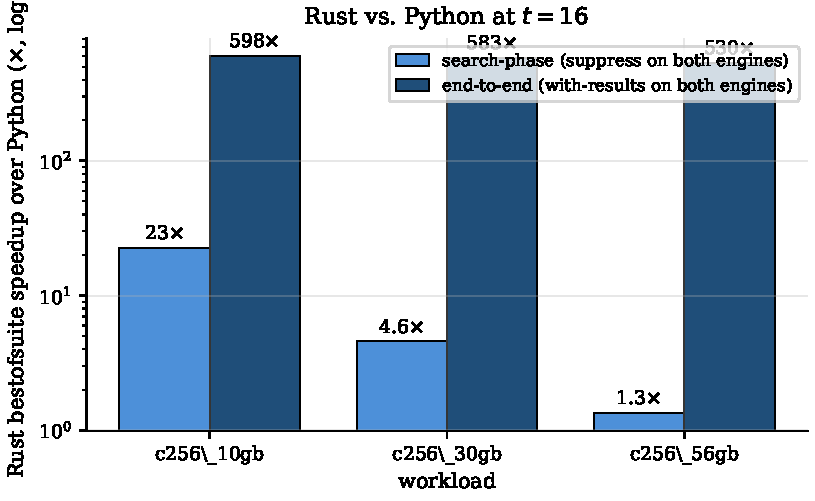
\includegraphics[width=0.9\linewidth]{img/gen/ch4_e2e_speedup.pdf}
  \caption{Rust \bcombo{} speedup over the Python baseline at $t=16$ across the three calibration workloads, End-to-end (with-results) stays in the $530$--$598\times$ range because of Python's per-\emph{(query, cluster)} result-dict construction. Search phase alone (suppress) drops monotonically from $22.7\times$ $\to$ $1.34\times$. Log $y$-axis.}
  \label{fig:exp:e2e_speedup}
\end{figure}

\section{Rust Rebinning Kernel\label{sec:exp:rebinning}}

We fuse the two stages of the Python rebinning (per-histogram rebinning under \texttt{multiprocessing.Pool}, then \texttt{numpy.cumsum} + \texttt{argsort(axis=0)} per cluster) into a single-threaded, in-place Rust call. Rust parallelizes the rebinning across all cores, followed by in-place cumsum and a stable \texttt{sort\_by}.

\begin{table}[H]
  \centering
  \caption{Rebinning kernel wall across the three calibration datasets, median of 3 reps.}
  \label{tab:rebin}
  \footnotesize
  \begin{tabular}{lrrr}
    \toprule
    Dataset & Python (\texttt{multiprocessing.Pool}) & Rust kernel & Speedup \\
    \midrule
    \texttt{c256\_10gb} ($324$\,K hists) & $83.5$\,s & $17.7$\,s & $4.72\times$ \\
    \texttt{c256\_30gb} ($997$\,K hists) & $306.5$\,s & $64.3$\,s & $4.77\times$ \\
    \texttt{c256\_56gb} ($5.02$\,M hists) & $3{,}220$\,s & $1{,}479$\,s & $2.18\times$ \\
    \bottomrule
  \end{tabular}
\end{table}

Correctness is verified against the Python reference on $200$ queries: the rounding-mode difference between Rust (round-half-away) and NumPy (banker's rounding) produces a maximum cumulative difference of $10^{-4}$ at a handful of histogram rows, which does not affect sort order or query results.

The kernel falls back to the Python pipeline if \texttt{fainder\_core} is not importable or if \texttt{bin\_estimation == \textquotesingle cubic\_spline\textquotesingle}.

\section{Variance Check on Borderline Claims\label{sec:exp:variance}}

Most claims in this chapter are far outside the noise floor, but a few are close enough to the noise floor that they were re-measured at $10$ reps per cell to tighten the interval, and one claim was re-verified against a variance probe.

\textbf{Fine-t f16 vs default on \texttt{c256\_56gb}} (§\ref{sec:exp:c2:f16}). Initially, under the $5$-rep sweep, the peak win was $\sim\!-10\%$ at $t{=}18$, but the $10$-rep upgrade brings the CI half-width from $\sim\!3.4\%$ to $\sim\!2.1\%$. Concluding that no cell shows a significant f16 standalone win.

\textbf{c1024 SIMD anomaly at $t{=}64$} (§\ref{sec:exp:ood:struct}). The $5$-rep sweep showed SIMD at $t{=}64$ measuring $-6.7\%$ vs baseline, an outlier to the $6/6$ null SIMD reproduction. The variance-probe run suggests the $t{=}64$ cell has anomalously high inter-run variance on this specific dataset.

\section{Summary\label{sec:exp:summary}}

Table~\ref{tab:exp:hyp_verdicts} revisits the a-priori hypotheses of §\ref{sec:method:hypotheses} against this chapter's evidence.

\begin{table}[H]
  \centering
  \caption{Hypotheses from Chapter~\ref{cha:chapter3} and their verdicts.}
  \label{tab:exp:hyp_verdicts}
  \footnotesize
  \begin{tabular}{>{\raggedright\arraybackslash}p{0.30\linewidth}>{\raggedright\arraybackslash}p{0.16\linewidth}>{\raggedright\arraybackslash}p{0.42\linewidth}}
    \toprule
    Hypothesis & Verdict & Evidence \\
    \midrule
    (i) Latency-side throughput reduces wall at every $t$ & Falsified & Four null ablations, $0.90$--$1.13\times$ across all cells (§\ref{sec:exp:c1}) \\
    (ii) Footprint reduction wins at intermediate $t$ & Refined & Binding constraint is regime-dependent: arena-mutex contention on the primary workload, L3-aggregate footprint at the OOD density; \texttt{f16} and \texttt{pooled} sign-flip inside the bundle (§\ref{sec:exp:c2}) \\
    (iii) Bandwidth reduction wins at high $t$ & Confirmed standalone; falsified in composition & \texttt{packed-ids} $-20\%$ standalone at high $t$; regresses over \bcombo{} in 12/18 cells (§\ref{sec:exp:c3}, §\ref{sec:exp:negcomp:instances}) \\
    (iv) NUMA probe separates on-socket pressure from UPI & Confirmed & Single-socket $-11$ to $-13\%$; interleave $+26$ to $+41\%$ (§\ref{sec:exp:c4}) \\
    Five predictions of positive composition & All falsified & Five instances on five hardware axes (§\ref{sec:exp:negcomp:instances}) \\
    Dispatch within $5\%$ in-distribution & Confirmed & $17/18$ exact, $18/18$ within $5\%$ (§\ref{sec:exp:dispatch}) \\
    OOD generalisation at the sparser density point & Confirmed & $6/6$ within $1\%$; $4$ strong $+$ $2$ clean reproductions, $2$ refinements, $0$ falsifications (§\ref{sec:exp:ood}) \\
    \bottomrule
  \end{tabular}
\end{table}

Four ceilings bind Fainder's percentile workload on this platform: single-thread compute / L1 latency (which never binds in practice), shared L3 capacity, on-socket memory-traffic pressure, and the cross-socket UPI interconnect. The latency-side optimisations (SIMD, batch-search, horizontal-SIMD, PGM) all measure null: they accelerate a stage that does not bind. The bandwidth-side optimisations (\texttt{f16}, \texttt{packed-ids}, \texttt{pooled}, \texttt{mimalloc}) and single-socket placement each move wall on their own ceiling.

These optimisations compose negatively. We show five instances on five hardware axes with respective \emph{perf} counters as evidence. It shows: the ceiling that binds at the composition is \emph{not} the one the second ablation attacks. This leads to the pre-flight methodology, where we probe the binding ceiling at the target composition before committing to an implementation.

The dispatch policy holds in-distribution ($17/18$ exact, $18/18$ within $5\%$) and out-of-distribution ($6/6$ within $5\%$ at $3.2\times$ sparser clusters). Ceilings (i) and (iv) reproduce across density while ceiling (ii) has a density-dependent threshold. Four of the five negative-composability instances reproduce in sign at the OOD point, and morsel scheduling attenuates to within-noise.

The Rust port that carried these measurements delivers $530$--$598\times$ end-to-end over the Python baseline at $t=16$, and $114\times$ at the only paired single-thread cell. Most of that ratio is Python's per-\emph{(query, cluster)} result materialisation ($96.9$--$99.8\%$ of its wall, §\ref{sec:exp:e2e:mat}). The search phase itself scales $22.7\times$, $4.6\times$, $1.34\times$ as per-cluster footprint grows into the shared ceilings. NUMA placement adds $11$--$13\%$ at $t \leq 48$, and the rebinning kernel a separate $\sim\!4.7\times$, dropping to $\sim\!2.2\times$ at five million histograms (§\ref{sec:exp:rebinning}).

What generalises beyond this codebase is the ceiling characterisation, the composition pattern, and the pre-flight methodology. The Rust port is the medium that produced them.
    \chapter{Related Work\label{cha:chapter5}}

In this chapter, we survey work related to the thesis's contributions in four directions: 

\begin{itemize}
    \item hardware-conscious index structures, 
    \item vectorised and parallel query processing, 
    \item approximate histogram-based systems, and 
    \item the performance engineering of Python-based data systems.
\end{itemize}

\section{Hardware-Optimised Index Structures}

Work done by Manegold et al.~\cite{manegold_2000} illustrates that main-memory access is the dominant bottleneck for in-memory database operations, from that work cache-conscious design principles were established, which subsequently influenced much of the work in database systems. Manegold et al.'s analysis showed that column-major (SoA) storage dramatically outperforms row-major (AoS) storage for projective (columnar) access patterns, which is the direct motivation for the memory layout designed in Chapter~\ref{cha:chapter3}.

Adaptive Radix Trees (ART)~\cite{leis_2013} adapt their node fanout to the key distribution, achieving cache efficiency for point and range queries. They avoid fixed-fanout waste of classical B-trees. ARTs target key-value loops rather than percentile predicate evaluations, nonetheless their design philosophy of having a data structure based on cache line behaviour rather than asymptotic complexity informs the approach taken in this thesis.

Khuong and Morin~\cite{khuong_morin_2017} established in a survey for comparison-based searching on modern CPUs that the Eytzinger layout (which is breadth-first) outperforms classical sorted arrays when workloads are cache-cold and of moderate size, due to its cache-line-aligned root of the search tree. This analysis was extended by Schlegel et al.~\cite{schlegel_2009} with SIMD-accelerated k-ary search. Neither of these constructions survived into the final integrated Fainder build, due to Fainder's elimination of cache-coldness on L1-resident columns and the k-ary chain shortening landing on the slack outside of $t=1$. The foundational analysis behind these designs traces back to Brodal and Fagerberg~\cite{brodal_fagerberg_2006}.

A learned index structure~\cite{kraska_2018} replaces B-tree index nodes with learned models that predict key positions. This trades worst-case guarantees (e.g. logarithmic search time) for expected-case cache efficiency. The problem with learned indexes is that they are only effective on learnable key distributions, that is documented by Kraska et al.~\cite{kraska_2018}. Classical sorted-array search with layouts that are hardware-conscious outperform these types of indexes when the key distribution is heterogeneous and cannot be accurately approximated by a small model. Fainder's histogram collection is exactly a heterogeneous workload, which is why classical binary search with SoA layout is the right choice.


\section{Vectorised and Parallel Query Processing}

For analytical queries, Neumann~\cite{neumann_2011} demonstrated that compiling query plans to native machine code rather than interpreting them through a tuple-at-a-time Volcano model yields order-of-magnitude performance improvements. Key insight here is that inner loops that are tight and specialised by type can be optimised by LLVM better than interpreted bytecode. The entire idea of Fainder's Rust implementation is motivated by this insight.

Kersten et al.~\cite{kersten_2018} compared compiled and vectorised query-execution models and found that neither dominates: vectorised execution wins where cache-resident batch processing and parallel data access matter, compilation where per-tuple work is tight. We implement explicit AVX-512 SIMD intrinsics for the final stage of Fainder's binary search (Section~\ref{sec:exp:c1:simd}), replacing the last ${\sim}16$ scalar iterations with a single vector comparison.

Leis et al.~\cite{leis_2014} showed with morsel-driven parallelism that dynamic work distribution outperforms static task partitioning when sub-tasks have unequal cost. Fainder's cluster queries have costs that are heterogeneous in exactly this way (large cluster $\to$ more histograms $\to$ more binary search steps). This leads us to choose Rayon's work stealing scheduler (an implementation of the scheduler of Blumofe and Leiserson~\cite{blumofe_leiserson_1999}) over round-robin thread assignment. Our reports in Chapter~\ref{cha:chapter4} are consistent with this: speedup grows with thread count until the memory-traffic and interconnect ceilings bind (§\ref{sec:exp:scaling}).

Kocberber et al.~\cite{kocberber_2013} propose a way to hide memory latency in in-memory hash-join traversal. This is possible by interleaving many independent lookups per core, saturating the MSHR budget. Fainder's 8-way batch binary search ablation (Section~\ref{sec:exp:c1:batch}) is a direct application of this idea. 


The MonetDB/X100 project~\cite{boncz_2005} introduced vector-at-a-time execution, processing cache-resident batches to combine columnar layouts with tight SIMD-friendly inner loops.  Section~\ref{sec:exp:wf:columnar} is inspired by this, and the  design is surveyed in a broader sense by Abadi et al.~\cite{abadi_2008,abadi_2013}. Vectorised database operators studied by Willhalm et al.~\cite{willhalm_2009} and Zhou and Ross~\cite{zhou_ross_2002} were also influential in Fainder's new SIMD design.

\section{Approximate Histogram-Based Systems}

Distribution queries are often approximated through compact histogram sketches. Data structures such as T-digest~\cite{dunning_2019} and HdrHistogram~\cite{hdrhistogram} maintain compressed representations of \emph{streaming} data distributions that support approximate quantile queries. Synopsis-based query processing~\cite{ioannidis_2003,cormode_2011} precomputes compact statistical summaries to answer approximate aggregate queries without scanning raw data.

We do not consider these systems as competitors to Fainder, since Fainder uses precomputed histograms to answer \emph{exact} percentile predicates, whereas the above systems target \emph{approximate} quantile computation over streaming or continuously updated data. A better classification would be that these are complementary systems: Fainder could be used to answer exact percentile queries on the histograms produced by these systems, or these systems could be used to generate the histograms that Fainder indexes.

\section{Hardware-Aware Indexing of Adjacent Primitives}

Percentile-predicate evaluation is a finer grained primitive than the hardware-conscious systems surveyed above, and it has not received the same level of attention. Below are several closely related primitives, that help us position Fainder's percentile-predicate evaluation in the landscape of hardware-conscious systems.

\textbf{Cache-resident sorted-array search.} Fainder's binary search runs against cache-resident data after warm-up: the bin-edge array (${\sim}142$ floats per cluster) is L1-resident, and the per-cluster cumulative-density slices range from L1- to L2-resident depending on cluster density (§\ref{sec:method:data}). The literature on cache-conscious sorted-array search is as follows:

\begin{itemize}
    \item Kim et al.'s FAST index~\cite{kim_2010} reports large speedups by re-organising search trees to exploit page size, cache-line size, and SIMD width simultaneously.
    \item Khuong and Morin~\cite{khuong_morin_2017}'s work shows small $n$ branchless binary search wins, while Eytzinger BFS layout wins for large $n$.
    \item Schlegel et al.'s k-ary search on modern processors~\cite{schlegel_2009} is the foundation for the SIMD k-ary variants explored in earlier ablation campaigns of this thesis, and for the SIMD leaf stage of Fainder's binary search (Section~\ref{sec:exp:c1:simd}).
\end{itemize}

\textbf{Vectorised column scan.} Fainder's f16 ablation (Section~\ref{sec:exp:c2:f16}) is a vectorised scan of a column of 16-bit floats, which is the same access pattern as the following systems:
\begin{itemize}
    \item BitWeaving~\cite{li_patel_2013} achieves below-one-cycle-per-element scan throughput by packing column values across word boundaries.
    \item ByteSlice~\cite{feng_2015} refines this with a byte-aligned layout.
\end{itemize}

Wallewein-Eising et al.~\cite{wallewein_2018} survey SIMD acceleration across main-memory index structures more broadly.

\section{Composability of Optimisations in Database and Systems Engineering}

The negative-composability pattern of §\ref{sec:exp:negcomp} reasons with three performance engineering perspectives.

\paragraph{Cost-based and adaptive query optimisation.} Selinger et al.~\cite{selinger_1979} formulated query optimisation with costs that decompose additively across operators. Adaptive query processing~\cite{avnur_hellerstein_2000} keeps the additive model, but defers plan selection to runtime statistics. We refine the scope of these assumptions with our five negative composition instances (§\ref{sec:exp:negcomp:instances}): at a ceiling, the cost of optimisation $B$ depends on which ceiling optimisation $A$ has already collected, so we can't rely on per-operator costs. In this case, the pre-flight check plays the same structural role as the Selinger cost model, based on perf counters rather than cardinalities, we apply a falsifiable predictor before committing to implementation cost.

\paragraph{Hardware--software co-design.}

Caladan and heartbeat scheduling~\cite{fried_2020_caladan,acar_2018_heartbeat} manage hardware interference inside a decision loop. They share the view that hardware ceilings bind performance, instead of algorithmic primitives. However, their reasoning for composition differs: Caladan assumes that along orthogonal resources, interference is independently manageable, and heartbeat scheduling assumes that the work composes, and that coordination overhead can be bounded under a work--span analysis. Our instance of a cooperative-cache scheduler over an already-amortised baseline (§\ref{sec:exp:wf:morsel}) is a counter-example: it satisfies the work--span analysis and still regresses, because no residual L3 misses remain to recover.

\paragraph{The ``no silver bullet'' and memory-wall traditions.}
Gains are assumed to compose multiplicatively in the ``no silver bullet'' tradition of Brooks~\cite{brooks_1987} and Wulf and McKee~\cite{wulf_mckee_1995}. While Brooks argues that the axes have to be independent, Wulf and McKee argue that the axes are not independent, but that the only way to get past the memory wall is to apply multiple hardware-conscious techniques. We show yet again, with our five negative-composition instances, that the axes are not independent, but that the right optimisation at each composition step is contingent on which ceiling currently binds.

\paragraph{Positioning.}
Each instance in the composition study (§\ref{sec:exp:negcomp:instances}) had an a-priori argument under each of these three perspectives that the composition should be positive. Each instance was then falsified by a perf-counter-grounded mechanism. There is, to our knowledge, no prior documentation of this specific shape: five axes, mechanism-grounded ablation pairs, and a falsifiable pre-flight diagnostic.


\section{Performance Gap in Distribution-Aware Search}

The original Fainder paper~\cite{behme_2024} does not benchmark against a compiled implementation, nor does it investigate hardware-level efficiency. Instead, it benchmarks against profile-scan, NDIST, PSCAN, and BinSort baselines and focuses on algorithmic correctness and retrieval effectiveness. The SIGMOD demo~\cite{behme_2025_demo}, the companion theoretical framework work of Esmailpour et al.~\cite{esmailpour_2025}, and the data-discovery survey of Esmailoghli, Galhotra, and Abedjan~\cite{abedjan_2025} situate Fainder (or Fainder-like work) algorithmically without addressing systems performance. Related distribution-aware systems suffer the same drawback: Esmailoghli et al.~\cite{EsmailoghliQZ21} and Traub et al.~\cite{TraubGCBKRM20} propose alternative indexing strategies without analysing cache or parallelism behaviour, Goods~\cite{halevy_2016} treats retrieval at indexing scale, Zhang and Ives~\cite{zhang_2018} focus on algorithmic structure, and Asudeh et al.~\cite{asudeh_2022} motivate metadata-rich search from a fairness angle.

The contribution of this thesis addresses two gaps of this literature:

\begin{itemize}
    \item No studies, to our knowledge, have been conducted that characterise hardware bottlenecks of histogram-based percentile search or hardware-conscious engineering of such systems.
    \item Before this work, no evaluation existed, to our knowledge, of inter-query SIMD for binary-search-shaped workloads at Fainder's cluster-loop scale on Sapphire Rapids. Existing evaluations such as Polychroniou et al.\ and Lang et al.~\cite{polychroniou_2014,lang_2020} predate the microarchitecture.
\end{itemize}

This thesis addresses the first gap with Fainder's query pipeline, due to its embarrassingly parallel structure, its access pattern being binary search, and its read-only index. It closes the second directly: the horizontal-SIMD evaluation of §\ref{sec:exp:c1:horizontal} is, to our knowledge, the first such measurement on Sapphire Rapids, with a null result at cache-resident scale.
    \chapter{Conclusion\label{cha:chapter6}}

\section{Summary}

This thesis overhauled Fainder's query execution pipeline into a compiled Rust extension module. The new engine was used for an ablation study across more than twenty hardware-conscious optimisation axes. The dominant outcome of this study is structural. The engineering speedup, while large, is mechanistically secondary to it.

On the Sapphire Rapids 8468H micro-architecture, Fainder's search phase is bound by four distinct performance ceilings: 

\begin{enumerate}
    \item Single-thread compute / L1 latency (\(t\leq 8\); candidate, refuted)
    \item Shared L3 capacity (\(t\approx 16\))
    \item On-socket memory-traffic pressure (\(t\in[32, 48]\) on one socket)
    \item Cross-socket UPI interconnect (\(t > 48\))
\end{enumerate}

Ceiling (i) is the literature's default assumption for binary-search workloads, its refutation on this workload is itself a finding. The ceilings were established through Chapter~\ref{cha:chapter4}'s perf counters. Ceiling (iii) and (iv) were separated by a four-configuration \texttt{numactl} probe.

Across five independent ablations on five different axes, a pattern emerged: a less fine-grained optimisation had already addressed the binding ceiling, and the finer-grained optimisation's overhead was a net regression rather than diminishing return. Although each instance had an argument to compose positively, each was falsified at scale by hardware counter evidence. The cross-axis breadth of the five instances rules out a per-axis coincidence and establishes the pattern as structural. The five ablations were: emit-phase ID packing over \bcombo{} (§\ref{sec:exp:c3:packed}), K-batch cluster amortisation over \texttt{f16} (§\ref{sec:exp:wf:qb}), morsel-driven phase coordination over query-batch (§\ref{sec:exp:wf:morsel}), per-cluster reindexing over packed-ids (§\ref{sec:exp:reindex}), and page-granular NUMA interleave over first-touch placement (§\ref{sec:exp:c4}). 

This pattern makes \textbf{dispatch-on-regime} the only near-optimal deployment strategy, which selects build features and deployment flags per workload regime. This dispatch policy was validated 17/18 exactly and 18/18 within 5\% in-distribution, and 6/6 within 5\% out-of-distribution, all six within 1\%, for a combined 23/24.

The engineering results are secondary to the structural finding: Rust achieves a $530$--$598\times$ end-to-end speedup over the Python baseline at the peak-scaling cell ($t=16$) across three independent dataset scales. This end-to-end ratio is dominated by Rust avoiding Python's result-dict construction (§\ref{sec:exp:e2e:mat}). The search phase itself scales from $22.7\times$ on the smallest calibration dataset to $1.34\times$ on the largest, bending the curve toward the shared hardware ceilings. All these speedups preserve precision $=$ recall $= 1.000$. The speedup depends on the regime, since negative composability makes the best composition for one regime, regress at another.

\section{Contributions}

The thesis makes five primary contributions.

\begin{enumerate}
    \item \textbf{Engineering re-implementation.} Rust port of Fainder's query execution pipeline, validated at precision $=$ recall $= 1.000$. Integrated into the existing Python API via PyO3, delivering a speedup across three independent dataset scales.
    
    \item \textbf{Four-ceiling characterisation.} Identification of four performance ceilings mentioned above, on the Sapphire Rapids 8468H micro-architecture, and the regimes under which each ceiling binds. 

    \item \textbf{Negative-composability pattern.} Five independent instances of composability where a second optimisation regresses at scale. An ablation that would compose positively would falsify this pattern.

    \item \textbf{Pre-flight ceiling-identification.} A probe template diagnoses the binding ceiling at the \emph{target composition} before committing to implementation. When multiple stacked ceilings exist, the ablation methodology (implement, measure, accept) is methodologically insufficient.
    
    \item \textbf{Dispatch-on-regime.} Automatic policy that selects build features and deployment flags per workload regime. Valid even across out-of-distribution scenarios.
\end{enumerate}

Contributions (1) and (5) are engineering artefacts, while (2), (3), and (4) are scientific and methodological findings.

\section{Limitations}

\paragraph{Single micro-architecture.}
All experiments run on a single Sapphire Rapids 8468H configuration. The ceilings introduced in this thesis are based on this micro-architecture. A different micro-architecture (Genoa, Granite Rapids, Grace) would most likely have different per-ceiling thresholds. The methodological contribution (pre-flight ceiling-identification) generalises across micro-architectures, the specific ceiling thresholds and dispatch policy entries do not.

\paragraph{Single-machine evaluation.}
All experiments run on shared memory. This might introduce a fifth ceiling of Network latency, in case of sharing the index across multiple machines. Asynchronous I/O and work offloading become candidate optimisations in that case.

\paragraph{Density-range scope.}
The dispatch-on-regime policy is validated at \(n_\text{hists}/n_\text{clusters}\) densities of $\sim$8,200 (c1024\_56gb) and $\sim$26,300 (c256\_56gb). The policy is not validated at densities below $\sim$8,200 (c4096\_56gb) or above $\sim$26,300 (c128\_56gb), both outside the validated range. The policy's density axis is therefore a prediction rather than a validated entry.

\section{Future Work}

Future work includes three experiments that would extend the structural findings.

\paragraph{(F1) Transparent Huge Pages probe across all builds.}
The §\ref{sec:exp:reindex} mechanism localised the local-ids regression. The bw=13 decoder's access pattern over the packed buffer drives page-walk pressure. With Transparent Huge Pages enabled ($2$\,MiB pages instead of $4$\,KiB), TLB-miss frequency drops by $512\times$ per covered page, and the page-walker's $\sim\!100$-cycle penalty per miss correspondingly shrinks.

\paragraph{(F2) NUMA-aware build for $t > 48$.}
§\ref{sec:exp:c4} identified cross-socket UPI as the fourth ceiling and showed that single-socket placement saves 11--13\% at $t \leq 48$. Single-socket placement is infeasible at $t >  48$ due to socket 0 having only 48 physical cores. A NUMA-aware build would shard the cluster set across the two sockets at index-load time and pin Rayon workers to physical cores within their NUMA node. Queries would then iterate over node-local clusters preferentially.

\paragraph{(F3) Smaller follow-ons.}

\textit{Adaptive precision selection.} Optimal f16 vs f32 precision depends on the regime. F32 wins at low $t$, while f16 wins at high $t$. An adaptive scheme at runtime that selects precision based on the thread count (or L3-miss rate) would provide the best of both.

\textit{Column-centric engine for small datasets.} Column-centric outperformed row-centric at $t=1$ by $2.17$--$2.63\times$ (§\ref{sec:exp:wf:columnar}). Broadening its win region would require addressing the cross-cluster load imbalance that causes columnar to lose by a factor of 2 at $t \geq 8$.

\section{Closing Remark}

The engineering speedups produced in this thesis are specific to this codebase, micro-architecture, and workload. The structural finding is what generalises. On hardware-near workloads the cost of regression for optimisation $B$ on an already applied optimisation $A$ depends on which ceiling has been collected already, making it invisible to per-operator cost models. This makes our finding clear: identify the binding ceiling at the target composition before committing the implementation cost of the next ablation.


% ---------------------------------------------------------------

%Bibliography
\begingroup
\raggedright
\bibliographystyle{splncs03}
%\bibliographystyle{acm}
\bibliography{bibliography}
\endgroup

%appendix
\addchap{Appendix A. Reproduction and Implementation Details}
\label{app:reproduction}

This appendix documents the hardware, software, and build configuration used for every measurement in Chapter~\ref{cha:chapter4}, and provides explicit reproduction recipes for each ablation.

\section*{A.1 Hardware}

\begin{itemize}
  \item \textbf{Server}: single shared-memory node (192 logical threads total).
  \item \textbf{CPU}: 2\,$\times$ Intel Xeon Platinum 8468H (Sapphire Rapids, 48 physical cores per socket, hyperthreading enabled, up to 2.1\,GHz base / 3.8\,GHz turbo).
  \item \textbf{Caches}: 48\,KB L1-dcache per core; 2\,MB L2 per core; 105\,MB L3 per socket (shared within a NUMA node).
  \item \textbf{NUMA}: two nodes, one per socket. Node~0 holds logical CPUs 0--47 and their hyperthread siblings 96--143; node~1 holds 48--95 and 144--191. The 48-physical-core-per-node bound is the reason thread counts $t \geq 64$ span both NUMA nodes.
  \item \textbf{Memory}: $\approx$1\,TB DDR5 across both sockets, eight channels per socket.
  \item \textbf{Storage}: NVMe SSD (dataset loads); \texttt{/dev/shm} RAM-backed tmpfs (storage-hierarchy ablation).
\end{itemize}

\section*{A.2 Software}

\begin{itemize}
  \item \textbf{OS}: Ubuntu 22.04.5 LTS, Linux kernel 5.15.0-176-generic, glibc 2.35.
  \item \textbf{Rust}: rustc 1.94.1 (LLVM 21.1.8). Cargo default \texttt{release} profile (\texttt{opt-level=3}); \texttt{-C target-cpu=native} supplied via \texttt{.cargo/config.toml}.
  \item \textbf{Python}: 3.10.12; NumPy 1.26.4; zstandard 0.22.0.
  \item \textbf{Rust crates} (Cargo.lock resolved): pyo3 0.22.6; numpy 0.22.1; rayon 1.11.0; ndarray 0.16.1; half 2.7.1; mimalloc 0.1.50; crossbeam-deque 0.8.6; thiserror 1.0.69.
  \item \textbf{Build tool}: Maturin 1.7. The Rust extension is compiled via \texttt{maturin develop --release [--features ...]} and installed into the active virtualenv.
  \item \textbf{Profiling}: Linux \texttt{perf} 5.15 (\texttt{/proc/sys/kernel/perf\_event\_paranoid = 1}).
\end{itemize}

\section*{A.3 Repository Structure}

The full repository layout is documented in the artefact's \texttt{README} (\url{https://github.com/tmukh/Fainder-Redone}). Rust engine lives under \texttt{src/}, the Python integration under \texttt{fainder/}, the benchmark drivers under \texttt{scripts/}, the figure-generation code under \texttt{analysis/}, and the raw measurement database under \texttt{logs/}.

\section*{A.4 Feature-Flag Matrix}

The Rust crate uses Cargo feature flags to compile alternative implementations of \texttt{SubIndex}, the search loop, and the parallelism strategy. Exactly one feature combination is active per build.

\footnotesize
\begin{tabular}{llp{7cm}}
  \toprule
  Flag & Default & Effect \\
  \midrule
  (none)         & yes & SoA layout, f32 values, stdlib \texttt{partition\_point}, query-level parallelism \\
  \texttt{aos}   & no  & Array-of-Structs layout: \texttt{Vec<(f32,u32)>} \\
  \texttt{f16}   & no  & Half-precision percentile values \\
  \texttt{cluster-par} & no & Nested \texttt{par\_iter} over clusters (documented negative result) \\
  \texttt{simd}  & no  & AVX-512 leaf-stage compare in the binary-search inner loop \\
  \texttt{batch-search} & no & 8-way interleaved binary search (columnar engine only) \\
  \texttt{horizontal-simd} & no & AVX-512 16-query horizontal lockstep \\
  \texttt{pgm}   & no  & PGM learned-index search \\
  \texttt{packed-ids} & no & Bit-packed per-cluster identifiers \\
  \texttt{local-ids}, \texttt{-bench}, \texttt{-noalloc} & no & Reindexed 13-bit local IDs (three mutually-exclusive variants) \\
  \texttt{pooled} & no & Pre-allocated per-query output buffer \\
  \texttt{pin-cores} & no & Rayon workers pinned to distinct physical cores \\
  \texttt{cluster-prefetch} & no & Software \texttt{\_mm\_prefetch} of cluster $c{+}1$ \\
  \texttt{mimalloc} & no & mimalloc allocator \\
  \texttt{query-batch} & no & Column-centric inner loop over K-query batches \\
  \texttt{morsel} & no & Chase--Lev deque phase-aligned scheduler \\
  \bottomrule
\end{tabular}

\vspace{0.5em}
\noindent The \texttt{eytzinger} and \texttt{kary} feature flags belong to an earlier campaign build and are not present in the final integrated build's \texttt{Cargo.toml}.

\section*{A.5 Reproduction Recipes}

All commands assume the working directory is the repository root and the Python virtualenv is activated (\texttt{source venv/bin/activate}).

\textbf{Dataset naming.} The shell scripts accept legacy datasets (\texttt{eval\_10gb}, \texttt{eval\_medium}, \texttt{dev\_small}) as CLI arguments, matching the on-disk dataset folder names on the measurement server. These map to the naming used throughout the thesis body and the measurement database as follows:

\footnotesize
\begin{tabular}{ll>{\raggedright\arraybackslash}p{5cm}}
  \toprule
  Script argument & Thesis name & Notes \\
  \midrule
  \texttt{eval\_10gb}   & \texttt{c256\_10gb}  & $K=256$, $\sim$10\,GB \\
  \texttt{eval\_medium} & \texttt{c256\_30gb}  & $K=256$, $\sim$30\,GB \\
  (built fresh)         & \texttt{c256\_56gb}  & $K=256$, $\sim$56\,GB, full workload \\
  (built fresh)         & \texttt{c1024\_56gb} & $K=1024$; reclusters \texttt{c256\_56gb} for the out-of-distribution probe \\
  \texttt{dev\_small}   & ---                  & Smoke test only; not used in results \\
  \bottomrule
\end{tabular}

\vspace{0.5em}

\textbf{Build.} The default (SoA + f32 + partition\_point) build is:
\begin{verbatim}
maturin develop --release
\end{verbatim}

For an ablation-specific build, pass the feature flag:
\begin{verbatim}
maturin develop --release --features f16
maturin develop --release \
    --features "pooled f16 simd pin-cores cluster-prefetch mimalloc"
\end{verbatim}

\textbf{Ablation runs.} Each ablation has a shell driver that (1) compiles the relevant build, (2) runs the thread sweep with \texttt{--suppress-results}, (3) extracts the \texttt{Rust index-based query execution time} per log, and (4) prints a summary table. Representative commands:

\begin{verbatim}
# Thread sweep (default build, 7 thread counts 1-64)
bash scripts/ablation_parallel.sh eval_medium

# f16 vs f32 (rebuilds twice)
bash scripts/ablation_f16.sh eval_medium

# Columnar vs row-centric
bash scripts/ablation_columnar.sh eval_medium

# NUMA pinning
bash scripts/ablation_numa.sh eval_medium
\end{verbatim}

\textbf{Perf counters.} The perf-stat runs use \texttt{--delay=40000} to skip the $\sim$35\,s of load+init+warmup, and repeat the measured query set five times to avoid under-sampling:

\begin{verbatim}
bash scripts/perf_comprehensive.sh eval_medium
bash scripts/perf_branch_misses.sh
\end{verbatim}

\textbf{Figure regeneration.} Figures are regenerated from the measurement logs without re-running the experiments:

\begin{verbatim}
python analysis/plot_all_results.py
python analysis/plot_hardware_ablation.py
\end{verbatim}

\section*{A.6 Query Metric}

All ablation runs use \texttt{suppress\_results=True}, which returns empty result vectors while still executing the full binary-search work. This isolates search time from the Python set-building phase that dominated pre-PyO3-fix measurements and would otherwise swamp engineering-scale differences between variants. The extracted metric is the log line emitted by the Rust backend:

\begin{verbatim}
Rust index-based query execution time: X.XXXs
\end{verbatim}

This represents the wall-clock time of the Rayon-parallel query phase only, excluding the one-time \texttt{FainderIndex} construction from NumPy arrays ($\sim$17\,s on \texttt{eval\_medium}) and the initial index load (0.013\,s via mmap).


\end{document}
